%% Run LaTeX on this file several times to get Table of Contents,
%% cross-references, and citations.

\documentclass[11pt]{book}
\usepackage{gvv-book}
%\usepackage{Wiley-AuthoringTemplate}
\usepackage[sectionbib,authoryear]{natbib}% for name-date citation comment the below line
%\usepackage[sectionbib,numbers]{natbib}% for numbered citation comment the above line

%%********************************************************************%%
%%       How many levels of section head would you like numbered?     %%
%% 0= no section numbers, 1= section, 2= subsection, 3= subsubsection %%
\setcounter{secnumdepth}{3}
%%********************************************************************%%
%%**********************************************************************%%
%%     How many levels of section head would you like to appear in the  %%
%%				Table of Contents?			%%
%% 0= chapter, 1= section, 2= subsection, 3= subsubsection titles.	%%
\setcounter{tocdepth}{2}
%%**********************************************************************%%

%\includeonly{ch01}
\makeindex

\begin{document}

\frontmatter
%%%%%%%%%%%%%%%%%%%%%%%%%%%%%%%%%%%%%%%%%%%%%%%%%%%%%%%%%%%%%%%%
%% Title Pages
%% Wiley will provide title and copyright page, but you can make
%% your own titlepages if you'd like anyway
%% Setting up title pages, type in the appropriate names here:

\booktitle{Digital Communication}

\subtitle{Through Simulations}

\AuAff{G. V. V. Sharma}


%% \\ will start a new line.
%% You may add \affil{} for affiliation, ie,
%\authors{Robert M. Groves\\
%\affil{Universitat de les Illes Balears}
%Floyd J. Fowler, Jr.\\
%\affil{University of New Mexico}
%}

%% Print Half Title and Title Page:
%\halftitlepage
\titlepage

%%%%%%%%%%%%%%%%%%%%%%%%%%%%%%%%%%%%%%%%%%%%%%%%%%%%%%%%%%%%%%%%
%% Copyright Page

\begin{copyrightpage}{2022}
%Title, etc
\end{copyrightpage}

% Note, you must use \ to start indented lines, ie,
% 
% \begin{copyrightpage}{2004}
% Survey Methodology / Robert M. Groves . . . [et al.].
% \       p. cm.---(Wiley series in survey methodology)
% \    ``Wiley-Interscience."
% \    Includes bibliographical references and index.
% \    ISBN 0-471-48348-6 (pbk.)
% \    1. Surveys---Methodology.  2. Social 
% \  sciences---Research---Statistical methods.  I. Groves, Robert M.  II. %
% Series.\\

% HA31.2.S873 2004
% 001.4'33---dc22                                             2004044064
% \end{copyrightpage}

%%%%%%%%%%%%%%%%%%%%%%%%%%%%%%%%%%%%%%%%%%%%%%%%%%%%%%%%%%%%%%%%
%% Only Dedication (optional) 

%\dedication{To my parents}

\tableofcontents

%\listoffigures %optional
%\listoftables  %optional

%% or Contributor Page for edited books
%% before \tableofcontents

%%%%%%%%%%%%%%%%%%%%%%%%%%%%%%%%%%%%%%%%%%%%%%%%%%%%%%%%%%%%%%%%
%  Contributors Page for Edited Book
%%%%%%%%%%%%%%%%%%%%%%%%%%%%%%%%%%%%%%%%%%%%%%%%%%%%%%%%%%%%%%%%

% If your book has chapters written by different authors,
% you'll need a Contributors page.

% Use \begin{contributors}...\end{contributors} and
% then enter each author with the \name{} command, followed
% by the affiliation information.

% \begin{contributors}
% \name{Masayki Abe,} Fujitsu Laboratories Ltd., Fujitsu Limited, Atsugi, Japan
%
% \name{L. A. Akers,} Center for Solid State Electronics Research, Arizona State University, Tempe, Arizona
%
% \name{G. H. Bernstein,} Department of Electrical and Computer Engineering, University of Notre Dame, Notre Dame, South Bend, Indiana; formerly of
% Center for Solid State Electronics Research, Arizona
% State University, Tempe, Arizona 
% \end{contributors}

%%%%%%%%%%%%%%%%%%%%%%%%%%%%%%%%%%%%%%%%%%%%%%%%%%%%%%%%%%%%%%%%
% Optional Foreword:

%\begin{foreword}
%\lipsum[1-2]
%\end{foreword}

%%%%%%%%%%%%%%%%%%%%%%%%%%%%%%%%%%%%%%%%%%%%%%%%%%%%%%%%%%%%%%%%
% Optional Preface:

%\begin{preface}
%\lipsum[1-1]
%\prefaceauthor{}
%\where{place\\
% date}
%\end{preface}

% ie,
% \begin{preface}
% This is an example preface.
% \prefaceauthor{R. K. Watts}
% \where{Durham, North Carolina\\
% September, 2004}

%%%%%%%%%%%%%%%%%%%%%%%%%%%%%%%%%%%%%%%%%%%%%%%%%%%%%%%%%%%%%%%%
% Optional Acknowledgments:

%\acknowledgments
%\lipsum[1-2]
%\authorinitials{I. R. S.}  

%%%%%%%%%%%%%%%%%%%%%%%%%%%%%%%%
%% Glossary Type of Environment:

% \begin{glossary}
% \term{<term>}{<description>}
% \end{glossary}

%%%%%%%%%%%%%%%%%%%%%%%%%%%%%%%%
%\begin{acronyms}
%\acro{ASTA}{Arrivals See Time Averages}
%\acro{BHCA}{Busy Hour Call Attempts}
%\acro{BR}{Bandwidth Reservation}
%\acro{b.u.}{bandwidth unit(s)}
%\acro{CAC}{Call / Connection Admission Control}
%\acro{CBP}{Call Blocking Probability(-ies)}
%\acro{CCS}{Centum Call Seconds}
%\acro{CDTM}{Connection Dependent Threshold Model}
%\acro{CS}{Complete Sharing}
%\acro{DiffServ}{Differentiated Services}
%\acro{EMLM}{Erlang Multirate Loss Model}
%\acro{erl}{The Erlang unit of traffic-load}
%\acro{FIFO}{First in - First out}
%\acro{GB}{Global balance}
%\acro{GoS}{Grade of Service}
%\acro{ICT}{Information and Communication Technology}
%\acro{IntServ}{Integrated Services}
%\acro{IP}{Internet Protocol}
%\acro{ITU-T}{International Telecommunication Unit -- Standardization sector}
%\acro{LB}{Local balance}
%\acro{LHS}{Left hand side}
%\acro{LIFO}{Last in - First out}
%\acro{MMPP}{Markov Modulated Poisson Process}
%\acro{MPLS}{Multiple Protocol Labeling Switching}
%\acro{MRM}{Multi-Retry Model}
%\acro{MTM}{Multi-Threshold Model}
%\acro{PASTA}{Poisson Arrivals See Time Averages}
%\acro{PDF}{Probability Distribution Function}
%\acro{pdf}{probability density function}
%\acro{PFS}{Product Form Solution}
%\acro{QoS}{Quality of Service}
%\acro{r.v.}{random variable(s)}
%\acro{RED}{random early detection}
%\acro{RHS}{Right hand side}
%\acro{RLA}{Reduced Load Approximation}
%\acro{SIRO}{service in random order}
%\acro{SRM}{Single-Retry Model}
%\acro{STM}{Single-Threshold Model}
%\acro{TCP}{Transport Control Protocol}
%\acro{TH}{Threshold(s)}
%\acro{UDP}{User Datagram Protocol}
%\end{acronyms}

\setcounter{page}{1}

\begin{introduction}
This book introduces digital communication through probability.

\end{introduction}

\mainmatter

\chapter{Two Dice}
\iffalse
\documentclass[journal,12pt,twocolumn]{IEEEtran}
%
\usepackage{setspace}
\usepackage{gensymb}
%\doublespacing
\singlespacing

%\usepackage{graphicx}
%\usepackage{amssymb}
%\usepackage{relsize}
\usepackage[cmex10]{amsmath}
\usepackage{siunitx}
%\usepackage{amsthm}
%\interdisplaylinepenalty=2500
%\savesymbol{iint}
%\usepackage{txfonts}
%\restoresymbol{TXF}{iint}
%\usepackage{wasysym}
\usepackage{amsthm}
\usepackage{mathrsfs}
\usepackage{txfonts}
\usepackage{stfloats}
\usepackage{steinmetz}
%\usepackage{bm}
\usepackage{cite}
\usepackage{cases}
\usepackage{subfig}
%\usepackage{xtab}
\usepackage{longtable}
\usepackage{multirow}
%\usepackage{algorithm}
%\usepackage{algpseudocode}
\usepackage{enumitem}
\usepackage{mathtools}
\usepackage{tikz}
\usepackage{circuitikz}
\usepackage{pgfplots}
\usepackage{verbatim}
\usepackage{tfrupee}
\usepackage[breaklinks=true]{hyperref}
%\usepackage{stmaryrd}
\usepackage{tkz-euclide} % loads  TikZ and tkz-base
%\usetkzobj{all}
\usetikzlibrary{calc,math}
\usetikzlibrary{fadings}
\usepackage{listings}
    \usepackage{color}                                            %%
    \usepackage{array}                                            %%
    \usepackage{longtable}                                        %%
    \usepackage{calc}                                             %%
    \usepackage{multirow}                                         %%
    \usepackage{hhline}                                           %%
    \usepackage{ifthen}                                           %%
  %optionally (for landscape tables embedded in another document): %%
    \usepackage{lscape}     
\usepackage{multicol}
\usepackage{chngcntr}
%\usepackage{enumerate}

%\usepackage{wasysym}
%\newcounter{MYtempeqncnt}
\DeclareMathOperator*{\Res}{Res}
%\renewcommand{\baselinestretch}{2}
\renewcommand\thesection{\arabic{section}}
\renewcommand\thesubsection{\thesection.\arabic{subsection}}
\renewcommand\thesubsubsection{\thesubsection.\arabic{subsubsection}}

\renewcommand\thesectiondis{\arabic{section}}
\renewcommand\thesubsectiondis{\thesectiondis.\arabic{subsection}}
\renewcommand\thesubsubsectiondis{\thesubsectiondis.\arabic{subsubsection}}

% correct bad hyphenation here
\hyphenation{op-tical net-works semi-conduc-tor}
\def\inputGnumericTable{}                                 %%

\lstset{
%language=C,
frame=single, 
breaklines=true,
columns=fullflexible
}
%\lstset{
%language=tex,
%frame=single, 
%breaklines=true
%}

\begin{document}
%


\newtheorem{theorem}{Theorem}[section]
\newtheorem{problem}{Problem}
\newtheorem{proposition}{Proposition}[section]
\newtheorem{lemma}{Lemma}[section]
\newtheorem{corollary}[theorem]{Corollary}
\newtheorem{example}{Example}[section]
\newtheorem{definition}[problem]{Definition}
%\newtheorem{thm}{Theorem}[section] 
%\newtheorem{defn}[thm]{Definition}
%\newtheorem{algorithm}{Algorithm}[section]
%\newtheorem{cor}{Corollary}
\newcommand{\BEQA}{\begin{eqnarray}}
\newcommand{\EEQA}{\end{eqnarray}}
\newcommand{\define}{\stackrel{\triangle}{=}}

\bibliographystyle{IEEEtran}
%\bibliographystyle{ieeetr}


\providecommand{\mbf}{\mathbf}
\providecommand{\pr}[1]{\ensuremath{\Pr\left(#1\right)}}
\providecommand{\qfunc}[1]{\ensuremath{Q\left(#1\right)}}
\providecommand{\sbrak}[1]{\ensuremath{{}\left[#1\right]}}
\providecommand{\lsbrak}[1]{\ensuremath{{}\left[#1\right.}}
\providecommand{\rsbrak}[1]{\ensuremath{{}\left.#1\right]}}
\providecommand{\brak}[1]{\ensuremath{\left(#1\right)}}
\providecommand{\lbrak}[1]{\ensuremath{\left(#1\right.}}
\providecommand{\rbrak}[1]{\ensuremath{\left.#1\right)}}
\providecommand{\cbrak}[1]{\ensuremath{\left\{#1\right\}}}
\providecommand{\lcbrak}[1]{\ensuremath{\left\{#1\right.}}
\providecommand{\rcbrak}[1]{\ensuremath{\left.#1\right\}}}
\theoremstyle{remark}
\newtheorem{rem}{Remark}
\newcommand{\sgn}{\mathop{\mathrm{sgn}}}
\providecommand{\abs}[1]{\left\vert#1\right\vert}
\providecommand{\res}[1]{\Res\displaylimits_{#1}} 
\providecommand{\norm}[1]{\left\lVert#1\right\rVert}
%\providecommand{\norm}[1]{\lVert#1\rVert}
\providecommand{\mtx}[1]{\mathbf{#1}}
\providecommand{\mean}[1]{E\left[ #1 \right]}
\providecommand{\fourier}{\overset{\mathcal{F}}{ \rightleftharpoons}}
%\providecommand{\hilbert}{\overset{\mathcal{H}}{ \rightleftharpoons}}
\providecommand{\ztrans}{\overset{\mathcal{Z}}{ \rightleftharpoons}}
\providecommand{\system}{\overset{\mathcal{H}}{ \longleftrightarrow}}
	%\newcommand{\solution}[2]{\textbf{Solution:}{#1}}
\newcommand{\solution}{\noindent \textbf{Solution: }}
\newcommand{\cosec}{\,\text{cosec}\,}
\providecommand{\dec}[2]{\ensuremath{\overset{#1}{\underset{#2}{\gtrless}}}}
\newcommand{\myvec}[1]{\ensuremath{\begin{pmatrix}#1\end{pmatrix}}}
\newcommand{\mydet}[1]{\ensuremath{\begin{vmatrix}#1\end{vmatrix}}}
\providecommand{\gauss}[2]{\mathcal{N}\ensuremath{\left(#1,#2\right)}}
%\providecommand{\system}[1]{\overset{\mathcal{#1}}{ \longleftrightarrow}}
\newcommand*{\permcomb}[4][0mu]{{{}^{#3}\mkern#1#2_{#4}}}
\newcommand*{\perm}[1][-3mu]{\permcomb[#1]{P}}
\newcommand*{\comb}[1][-1mu]{\permcomb[#1]{C}}
%\numberwithin{equation}{section}
\numberwithin{equation}{subsection}
%\numberwithin{problem}{section}
%\numberwithin{definition}{section}
\makeatletter
\@addtoreset{figure}{problem}
\makeatother

\let\StandardTheFigure\thefigure
\let\vec\mathbf
%\renewcommand{\thefigure}{\theproblem.\arabic{figure}}
\renewcommand{\thefigure}{\theproblem}
%\setlist[enumerate,1]{before=\renewcommand\theequation{\theenumi.\arabic{equation}}
%\counterwithin{equation}{enumi}


%\renewcommand{\theequation}{\arabic{subsection}.\arabic{equation}}

\def\putbox#1#2#3{\makebox[0in][l]{\makebox[#1][l]{}\raisebox{\baselineskip}[0in][0in]{\raisebox{#2}[0in][0in]{#3}}}}
     \def\rightbox#1{\makebox[0in][r]{#1}}
     \def\centbox#1{\makebox[0in]{#1}}
     \def\topbox#1{\raisebox{-\baselineskip}[0in][0in]{#1}}
     \def\midbox#1{\raisebox{-0.5\baselineskip}[0in][0in]{#1}}

\vspace{3cm}

\title{
Probability and Random Variables
}
\author{ G V V Sharma$^{*}$% <-this % stops a space
	\thanks{*The author is with the Department
		of Electrical Engineering, Indian Institute of Technology, Hyderabad
		502285 India e-mail:  gadepall@iith.ac.in. All content in this manual is released under GNU GPL.  Free and open source.}
	
}	
%\title{
%	\logo{Matrix Analysis through Octave}{\begin{center}\includegraphics[scale=.24]{tlc}\end{center}}{}{HAMDSP}
%}


% paper title
% can use linebreaks \\ within to get better formatting as desired
%\title{Matrix Analysis through Octave}
%
%
% author names and IEEE memberships
% note positions of commas and nonbreaking spaces ( ~ ) LaTeX will not break
% a structure at a ~ so this keeps an author's name from being broken across
% two lines.
% use \thanks{} to gain access to the first footnote area
% a separate \thanks must be used for each paragraph as LaTeX2e's \thanks
% was not built to handle multiple paragraphs
%

%\author{<-this % stops a space
%\thanks{}}
%}
% note the % following the last \IEEEmembership and also \thanks - 
% these prevent an unwanted space from occurring between the last author name
% and the end of the author line. i.e., if you had this:
% 
% \author{....lastname \thanks{...} \thanks{...} }
%                     ^------------^------------^----Do not want these spaces!
%
% a space would be appended to the last name and could cause every name on that
% line to be shifted left slightly. This is one of those "LaTeX things". For
% instance, "\textbf{A} \textbf{B}" will typeset as "A B" not "AB". To get
% "AB" then you have to do: "\textbf{A}\textbf{B}"
% \thanks is no different in this regard, so shield the last } of each \thanks
% that ends a line with a % and do not let a space in before the next \thanks.
% Spaces after \IEEEmembership other than the last one are OK (and needed) as
% you are supposed to have spaces between the names. For what it is worth,
% this is a minor point as most people would not even notice if the said evil
% space somehow managed to creep in.



% The paper headers
%\markboth{Journal of \LaTeX\ Class Files,~Vol.~6, No.~1, January~2007}%
%{Shell \MakeLowercase{\textit{et al.}}: Bare Demo of IEEEtran.cls for Journals}
% The only time the second header will appear is for the odd numbered pages
% after the title page when using the twoside option.
% 
% *** Note that you probably will NOT want to include the author's ***
% *** name in the headers of peer review papers.                   ***
% You can use \ifCLASSOPTIONpeerreview for conditional compilation here if
% you desire.




% If you want to put a publisher's ID mark on the page you can do it like
% this:
%\IEEEpubid{0000--0000/00\$00.00~\copyright~2007 IEEE}
% Remember, if you use this you must call \IEEEpubidadjcol in the second
% column for its text to clear the IEEEpubid mark.



% make the title area
\maketitle

\newpage

\tableofcontents

\bigskip

\renewcommand{\thefigure}{\theenumi}
\renewcommand{\thetable}{\theenumi}
%\renewcommand{\theequation}{\theenumi}

%\begin{abstract}
%%\boldmath
%In this letter, an algorithm for evaluating the exact analytical bit error rate  (BER)  for the piecewise linear (PL) combiner for  multiple relays is presented. Previous results were available only for upto three relays. The algorithm is unique in the sense that  the actual mathematical expressions, that are prohibitively large, need not be explicitly obtained. The diversity gain due to multiple relays is shown through plots of the analytical BER, well supported by simulations. 
%
%\end{abstract}
% IEEEtran.cls defaults to using nonbold math in the Abstract.
% This preserves the distinction between vectors and scalars. However,
% if the journal you are submitting to favors bold math in the abstract,
% then you can use LaTeX's standard command \boldmath at the very start
% of the abstract to achieve this. Many IEEE journals frown on math
% in the abstract anyway.

% Note that keywords are not normally used for peerreview papers.
%\begin{IEEEkeywords}
%Cooperative diversity, decode and forward, piecewise linear
%\end{IEEEkeywords}



% For peer review papers, you can put extra information on the cover
% page as needed:
% \ifCLASSOPTIONpeerreview
% \begin{center} \bfseries EDICS Category: 3-BBND \end{center}
% \fi
%
% For peerreview papers, this IEEEtran command inserts a page break and
% creates the second title. It will be ignored for other modes.
%\IEEEpeerreviewmaketitle

%\begin{abstract}
%This book provides a simple introduction to probability and random variables.   The contents are largely based on  NCERT textbooks from Class 9-12.
%\end{abstract}


%\section{Axioms of Probability}
%\iffalse
%\documentclass[class=article, crop=false]{standalone}
\documentclass{article}
\usepackage{amssymb,amsfonts,amsthm,amsmath}
\usepackage{enumitem}
\usepackage{hyperref,xcolor}
\hypersetup{
    colorlinks,
    urlcolor={black}  %black!50!blue
}
\providecommand{\pr}[1]{\ensuremath{\Pr\left(#1\right)}}
\providecommand{\cbrak}[1]{\ensuremath{\left\{#1\right\}}}
\newcommand{\solution}{\noindent \textbf{Solution: }}
%\newcommand{\varsol}{\noindent \textbf{Aliter: }}
\newcommand*{\permcomb}[4][0mu]{{{}^{#3}\mkern#1#2_{#4}}}
%\newcommand*{\perm}[1][-3mu]{\permcomb[#1]{P}}
\newcommand*{\comb}[1][-1mu]{\permcomb[#1]{C}}
\setlist[enumerate]{font=\small\bfseries}
\renewcommand\thefootnote{\textcolor{black}{\arabic{footnote}}}

\begin{document}

\title{PROBABILITY}
\author{\Large DIVYA SAI - FWC22094}
\date{}

\maketitle
\begin{enumerate}[label=13.\arabic{enumi}.\arabic{enumii}]%,ref=\thesection.\theenumi.\theenumi]
\numberwithin{equation}{enumi}
\setcounter{enumi}{1}
\setcounter{enumii}{6}
\fi
From the given information,
\begin{align}
	\pr{E} \pr{F}&=\frac{3}{5} \times \frac{9}{50}
\\
	\pr{E F}&=\frac{1}{50}
\\
	\implies \pr{E F} &\neq P(E) P(F)
\end{align}
$\therefore$ $E$ and $F$ are not independent events.

\fi
\section{Bernoulli }
\begin{enumerate}[label=\thesection.\arabic*.,ref=\thesection.\theenumi]
\numberwithin{equation}{enumi}
\numberwithin{figure}{enumi}
\item The pmf of a Bernoulli distribution is defined as
\begin{align}
	p_X(k) = 
	\begin{cases}
		q = 1-p & k = 0
		\\
		p & k = 1
		\\
		0 & \text{otherwise}
	\end{cases}
\end{align}
\item For a Bernoulli random variable $X$ with success probability $p$,
\begin{align}
M_X(z)= q+pz^{-1}
\end{align}
\item The mean of the Bernoulli distribution is 
\begin{align}
	E\brak{X} = p
\end{align}
\end{enumerate}
\section{Binomial Distribution}
\begin{enumerate}[label=\thesection.\arabic*.,ref=\thesection.\theenumi]
\numberwithin{equation}{enumi}
\numberwithin{figure}{enumi}
\item The Binomial distribution is defined as 
\begin{align}
X &= X_1+X_2+...+X_n,
\end{align}
Where $X_i$ are i.i.d bernoulli.
\item For a Binomial random variable $X$ with parameters $n,p$,
\begin{align}
\label{eq:mgf-binom}
M_X(z)= \brak{q+pz^{-1}}^n
\end{align}
\item The mean for the Binomial r.v. is
\begin{align}
\label{eq:mean-binom}
E\sbrak{X}= np
\end{align}
\solution
From 
\eqref{eq:mgf-mean}
and 
\eqref{eq:mgf-binom},
\begin{align}
E\sbrak{X} 
&= \frac{d(q + pz)^n}{dz}\vert_{z=1}
\\
&=np(q + pz)^{n-1}|_{z=1}
\\
&= np(q + p)^{n-1}
\end{align}
yielding
\eqref{eq:mean-binom}
\begin{align}
\because p+q=1
\end{align}
\end{enumerate}
%
\section{Uniform Distribution}
\begin{enumerate}[label=\thesection.\arabic*.,ref=\thesection.\theenumi]
\numberwithin{equation}{enumi}
\numberwithin{figure}{enumi}
\item  Let $X \in \cbrak{1,2,3,4,5,6}$ be the random variables representing the outcome for a die.  Assuming the die to be fair, the probability mass function (pmf) is expressed as 
\begin{align}
\label{eq:dice_pmf_xi}
p_{X}(n) = 
\begin{cases}
\frac{1}{6} & 1 \le n \le 6
\\
0 & otherwise
\end{cases}
\end{align}
\item The $Z$-transform of $X$ is given by 
\begin{align}
P_{X}(z) =  \frac{1}{6}\sum_{n = 1}^{6}z^{-n}
=\frac{z^{-1}\brak{1-z^{-6}}}{6\brak{1-z^{-1}}}, \quad \abs{z} > 1
\label{eq:dice_xiz}
\end{align}
upon summing up the geometric progression.  
\end{enumerate}
\section{Triangular Distribution}

\renewcommand{\theequation}{\theenumi}
\renewcommand{\thefigure}{\theenumi}
\begin{enumerate}[label=\thesection.\arabic*.,ref=\thesection.\theenumi]
\numberwithin{equation}{enumi}
\numberwithin{figure}{enumi}

%

\item The desired outcome is
\begin{align}
\label{eq:dice_xdef}
X &= X_1 + X_2,
\\
\implies X &\in \cbrak{1,2,\dots,12}
\end{align}
%
The objective is to show that
\begin{align}
p_X(n) \ne \frac{1}{11}
\label{eq:dice_wrong}
\end{align}
\item {\em Convolution: }
From \eqref{eq:dice_xdef},
\begin{align}
p_X(n) &= \pr{X_1 + X_2 = n} = \pr{X_1  = n -X_2}
\\
&= \sum_{k}^{}\pr{X_1  = n -k | X_2 = k}p_{X_2}(k)
\label{eq:dice_x_sum}
\end{align}
after unconditioning.  $\because X_1$ and $X_2$ are independent,
\begin{multline}
\pr{X_1  = n -k | X_2 = k} 
\\
= \pr{X_1  = n -k} = p_{X_1}(n-k)
\label{eq:dice_x1_indep}
\end{multline}
From \eqref{eq:dice_x_sum} and \eqref{eq:dice_x1_indep},
\begin{align}
p_X(n) = \sum_{k}^{}p_{X_1}(n-k)p_{X_2}(k) = p_{X_1}(n)*p_{X_2}(n)
\label{eq:dice_x_conv}
\end{align}
where $*$ denotes the convolution operation. 
%\cite{proakis_dsp}.  
Substituting from \eqref{eq:dice_pmf_xi}
in \eqref{eq:dice_x_conv},
\begin{align}
p_X(n) = \frac{1}{6}\sum_{k=1}^{6}p_{X_1}(n-k)= \frac{1}{6}\sum_{k=n-6}^{n-1}p_{X_1}(k)
\label{eq:dice_x_conv_x1}
\end{align}
\begin{align}
\because p_{X_1}(k) &= 0, \quad k \le 1, k \ge 6.
\end{align}
From \eqref{eq:dice_x_conv_x1},
%
\begin{align}
p_X(n) &= 
\begin{cases}
0 & n < 1
\\
\frac{1}{6}\sum_{k=1}^{n-1}p_{X_1}(k) &  1 \le n-1 \le  6
\\
\frac{1}{6}\sum_{k=n-6}^{6}p_{X_1}(k) & 1 < n-6 \le 6
\\
0 & n > 12
\end{cases}
\label{eq:dice_x_conv_cond}
\end{align}
Substituting from \eqref{eq:dice_pmf_xi} in \eqref{eq:dice_x_conv_cond},
\begin{align}
p_X(n) &= 
\begin{cases}
0 & n < 1
\\
\frac{n-1}{36} &  2 \le n \le  7
\\
\frac{13-n}{36} & 7 < n \le 12
\\
0 & n > 12
\end{cases}
\label{eq:dice_x_conv_final}
\end{align}
satisfying \eqref{eq:dice_wrong}.
\item {\em The $Z$-transform: }
	\iffalse
The $Z$-transform of $p_X(n)$ is defined as 
%\cite{proakis_dsp}
\begin{align}
P_X(z) = \sum_{n = -\infty}^{\infty}p_X(n)z^{-n}, \quad z \in \mathbb{C}
\label{eq:dice_xz}
\end{align}
%
From \eqref{eq:dice_pmf_xi} and \eqref{eq:dice_xz}, 
\begin{align}
P_{X_1}(z) =P_{X_2}(z) &= \frac{1}{6}\sum_{n = 1}^{6}z^{-n}
\\
&=\frac{z^{-1}\brak{1-z^{-6}}}{6\brak{1-z^{-1}}}, \quad \abs{z} > 1
\label{eq:dice_xiz}
\end{align}
upon summing up the geometric progression.  
\fi
%\cite{proakis_dsp}. 
From \eqref{eq:dice_xiz} and \eqref{eq:dice_xzprod_def},
\begin{align}
P_X(z) &= \cbrak{\frac{z^{-1}\brak{1-z^{-6}}}{6\brak{1-z^{-1}}}}^2
\\
&= \frac{1}{36}\frac{z^{-2}\brak{1-2z^{-6}+z^{-12}}}{\brak{1-z^{-1}}^2}
\label{eq:dice_xzprod}
\end{align}
Using the fact that 
%\cite{proakis_dsp}
\begin{align}
p_X(n-k) &\system{Z}P_X(z)z^{-k},
\\
nu(n)&\system{Z} \frac{z^{-1}}{\brak{1-z^{-1}}^2}
\end{align}
after some algebra, it can be shown that
%{\tiny
\begin{multline}
\frac{1}{36}\lsbrak{\brak{n-1}u(n-1) - 2 \brak{n-7}u(n-7)}
\\
\rsbrak{ +\brak{n-13}u(n-13)}
\\
\system{Z}
\frac{1}{36}\frac{z^{-2}\brak{1-2z^{-6}+z^{-12}}}{\brak{1-z^{-1}}^2}
\label{eq:dice_xz_closed}
\end{multline}
%}

where 
\begin{align}
u(n) =
\begin{cases}
1 & n \ge 0
\\
0 & n < 0
\end{cases}
\end{align}

From \eqref{eq:dice_xz}, \eqref{eq:dice_xzprod} and \eqref{eq:dice_xz_closed}
\begin{multline}
p_{X}(n) = \frac{1}{36}\lsbrak{\brak{n-1}u(n-1) 
}
\\
\rsbrak{- 2 \brak{n-7}u(n-7)+\brak{n-13}u(n-13)}
\end{multline}
which is the same as \eqref{eq:dice_x_conv_final}.  Note that  \eqref{eq:dice_x_conv_final} can be obtained from \eqref{eq:dice_xz_closed} using contour integration as well.
% \cite{proakis_dsp}.  

\item 
The experiment of rolling the dice was simulated using Python for 10000 samples.  These were generated using Python libraries for uniform distribution. The frequencies for each outcome were then used to compute the resulting pmf, which  is plotted in Figure \ref{fig:dice}.  The theoretical pmf obtained in \eqref{eq:dice_x_conv_final} is plotted for comparison.  
%
\begin{figure}[!ht]
\centering
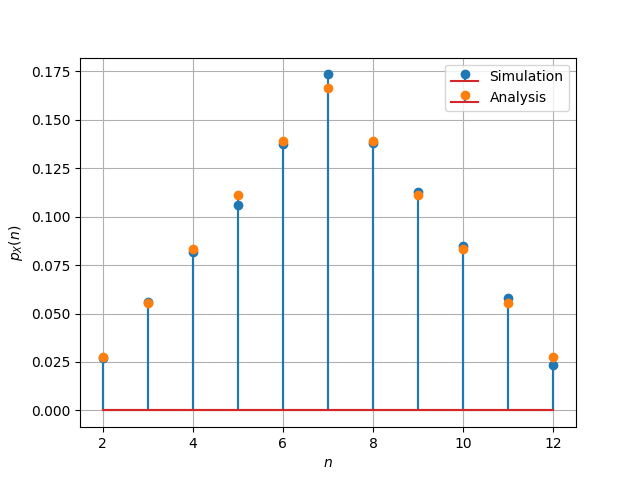
\includegraphics[width=\columnwidth]{./figs/sum/pmf.png}
\caption{Plot of $p_X(n)$.  Simulations are close to the analysis. }
\label{fig:dice}
\end{figure}
\item The python code is available below
	\lstinputlisting{codes/sum/dice.py}
	\iffalse
\begin{lstlisting}
/codes/sum/dice.py
\end{lstlisting}
\fi

%\item 
%We have shown how a simple problem of throwing a dice can be used for learning not just probability but concepts in  signal processing as well.  Inversion of the $Z$-transform for finding the pmf using contour integration, though not discussed here, opens a window to complex analysis too.  Note that the solutions that are provided  can be easily understood using high school math like arithmetic and geometric sums.  Thus, school students can use a bit of college level math to obtain simpler solutions to their problems.  College students can be exposed to advanced mathematics through simple problems from high school texts.  In addition, both can learn how to verify theoretical results through computer simulations.

%\bibliographystyle{tMES}
%\bibliography{school}
%
%\end{document}
\end{enumerate}



\chapter{Random Numbers}
\iffalse
\let\negmedspace\undefined
\let\negthickspace\undefined
\documentclass[journal,12pt,twocolumn]{IEEEtran}
%\documentclass[conference]{IEEEtran}
%\IEEEoverridecommandlockouts
% The preceding line is only needed to identify funding in the first footnote. If that is unneeded, please comment it out.
\usepackage{cite}
\usepackage{amssymb,amsfonts,amsthm,amsmath}
\usepackage{algorithmic}
\usepackage{graphicx}
\usepackage{textcomp}
\usepackage{xcolor}
\usepackage{txfonts}
\usepackage{listings}
\usepackage{enumitem}
\usepackage{mathtools}
\usepackage{gensymb}

%%
%\usepackage{setspace}
%%\doublespacing
%\singlespacing
%
%%\usepackage{graphicx}
%%\usepackage{amssymb}
%%\usepackage{relsize}
%\usepackage[cmex10]{amsmath}
%%\interdisplaylinepenalty=2500
%%\savesymbol{iint}
%%\usepackage{txfonts}
%%\restoresymbol{TXF}{iint}
%%\usepackage{wasysym}
%\usepackage{amsthm}
%\usepackage{mathrsfs}
%\usepackage{txfonts}
%%\usepackage{stfloats}
%%\usepackage{cite}
%%\usepackage{cases}
%%\usepackage{subfig}
%%\usepackage{xtab}
%%\usepackage{multirow}
%%\usepackage{algorithm}
%%\usepackage{algpseudocode}
%%\usepackage{tikz}
%%\usepackage{circuitikz}
%%\usepackage{verbatim}
\usepackage{hyperref}
%%\usepackage{stmaryrd}
%%\usepackage{tkz-euclide} % loads  TikZ and tkz-base
%%\usetkzobj{all}
    \usepackage{color}                                            %%
    \usepackage{array}                                            %%
    \usepackage{longtable}                                        %%
    \usepackage{calc}                                             %%
    \usepackage{multirow}                                         %%
    \usepackage{hhline}                                           %%
    \usepackage{ifthen}                                           %%
%  %optionally (for landscape tables embedded in another document): %%
%    \usepackage{lscape}     
%%\usepackage{multicol}
%\usepackage{chngcntr}
%\usepackage{enumerate}

%\usepackage{wasysym}
%\newcounter{MYtempeqncnt}
\DeclareMathOperator*{\Res}{Res}
%\renewcommand{\baselinestretch}{2}
\renewcommand\thesection{\arabic{section}}
\renewcommand\thesubsection{\thesection.\arabic{subsection}}
\renewcommand\thesubsubsection{\thesubsection.\arabic{subsubsection}}

\renewcommand\thesectiondis{\arabic{section}}
\renewcommand\thesubsectiondis{\thesectiondis.\arabic{subsection}}
\renewcommand\thesubsubsectiondis{\thesubsectiondis.\arabic{subsubsection}}

% correct bad hyphenation here
\hyphenation{op-tical net-works semi-conduc-tor}
\def\inputGnumericTable{}                                 %%

\lstset{
language=tex,
frame=single, 
breaklines=true
}

\begin{document}
%


\newtheorem{theorem}{Theorem}[section]
\newtheorem{problem}{Problem}
\newtheorem{proposition}{Proposition}[section]
\newtheorem{lemma}{Lemma}[section]
\newtheorem{corollary}[theorem]{Corollary}
\newtheorem{example}{Example}[section]
\newtheorem{definition}[problem]{Definition}
%\newtheorem{thm}{Theorem}[section] 
%\newtheorem{defn}[thm]{Definition}
%\newtheorem{algorithm}{Algorithm}[section]
%\newtheorem{cor}{Corollary}
\newcommand{\BEQA}{\begin{eqnarray}}
\newcommand{\EEQA}{\end{eqnarray}}
\newcommand{\define}{\stackrel{\triangle}{=}}

\bibliographystyle{IEEEtran}
%\bibliographystyle{ieeetr}


\providecommand{\mbf}{\mathbf}
\providecommand{\pr}[1]{\ensuremath{\Pr\left(#1\right)}}
\providecommand{\re}[1]{\ensuremath{\text{Re}\left(#1\right)}}
\providecommand{\im}[1]{\ensuremath{\text{Im}\left(#1\right)}}
\providecommand{\qfunc}[1]{\ensuremath{Q\left(#1\right)}}
\providecommand{\sbrak}[1]{\ensuremath{{}\left[#1\right]}}
\providecommand{\lsbrak}[1]{\ensuremath{{}\left[#1\right.}}
\providecommand{\rsbrak}[1]{\ensuremath{{}\left.#1\right]}}
\providecommand{\brak}[1]{\ensuremath{\left(#1\right)}}
\providecommand{\lbrak}[1]{\ensuremath{\left(#1\right.}}
\providecommand{\rbrak}[1]{\ensuremath{\left.#1\right)}}
\providecommand{\cbrak}[1]{\ensuremath{\left\{#1\right\}}}
\providecommand{\lcbrak}[1]{\ensuremath{\left\{#1\right.}}
\providecommand{\rcbrak}[1]{\ensuremath{\left.#1\right\}}}
\theoremstyle{remark}
\newtheorem{rem}{Remark}
\newcommand{\sgn}{\mathop{\mathrm{sgn}}}
\providecommand{\abs}[1]{\left\vert#1\right\vert}
\providecommand{\res}[1]{\Res\displaylimits_{#1}} 
\providecommand{\norm}[1]{\left\lVert#1\right\rVert}
%\providecommand{\norm}[1]{\lVert#1\rVert}
\providecommand{\mtx}[1]{\mathbf{#1}}
\providecommand{\mean}[1]{E\left[ #1 \right]}
\providecommand{\fourier}{\overset{\mathcal{F}}{ \rightleftharpoons}}
%\providecommand{\hilbert}{\overset{\mathcal{H}}{ \rightleftharpoons}}
\providecommand{\system}{\overset{\mathcal{H}}{ \longleftrightarrow}}
	%\newcommand{\solution}[2]{\textbf{Solution:}{#1}}
\newcommand{\solution}{\noindent \textbf{Solution: }}
\providecommand{\dec}[2]{\ensuremath{\overset{#1}{\underset{#2}{\gtrless}}}}
\newcommand{\myvec}[1]{\ensuremath{\begin{pmatrix}#1\end{pmatrix}}}
\newcommand{\mydet}[1]{\ensuremath{\begin{vmatrix}#1\end{vmatrix}}}
	\newcommand*{\permcomb}[4][0mu]{{{}^{#3}\mkern#1#2_{#4}}}
\newcommand*{\perm}[1][-3mu]{\permcomb[#1]{P}}
\newcommand*{\comb}[1][-1mu]{\permcomb[#1]{C}}
\providecommand{\gauss}[2]{\mathcal{N}\ensuremath{\left(#1,#2\right)}}
%%
%	%\newcommand{\solution}[2]{\textbf{Solution:}{#1}}
%\newcommand{\solution}{\noindent \textbf{Solution: }}
\newcommand{\cosec}{\,\text{cosec}\,}
\newcommand{\sinc}{\,\text{sinc}\,}
\newcommand{\rect}{\,\text{rect}\,}

%\numberwithin{equation}{section}
\numberwithin{equation}{subsection}
%\numberwithin{problem}{section}
%\numberwithin{definition}{section}
\makeatletter
\@addtoreset{figure}{problem}
\makeatother

\let\StandardTheFigure\thefigure
\let\vec\mathbf
\let\j\jmath
%\renewcommand{\thefigure}{\theproblem.\arabic{figure}}
\renewcommand{\thefigure}{\theproblem}
%\setlist[enumerate,1]{before=\renewcommand\theequation{\theenumi.\arabic{equation}}
%\counterwithin{equation}{enumi}


%\renewcommand{\theequation}{\arabic{subsection}.\arabic{equation}}

\def\putbox#1#2#3{\makebox[0in][l]{\makebox[#1][l]{}\raisebox{\baselineskip}[0in][0in]{\raisebox{#2}[0in][0in]{#3}}}}
     \def\rightbox#1{\makebox[0in][r]{#1}}
     \def\centbox#1{\makebox[0in]{#1}}
     \def\topbox#1{\raisebox{-\baselineskip}[0in][0in]{#1}}
     \def\midbox#1{\raisebox{-0.5\baselineskip}[0in][0in]{#1}}

\vspace{3cm}

\title{
%	\logo{
	Probability
%	}
}
%\title{
%	\logo{Matrix Analysis through Octave}{\begin{center}\includegraphics[scale=.24]{tlc}\end{center}}{}{HAMDSP}
%}


% paper title
% can use linebreaks \\ within to get better formatting as desired
%\title{Matrix Analysis through Octave}
%
%
% author names and IEEE memberships
% note positions of commas and nonbreaking spaces ( ~ ) LaTeX will not break
% a structure at a ~ so this keeps an author's name from being broken across
% two lines.
% use \thanks{} to gain access to the first footnote area
% a separate \thanks must be used for each paragraph as LaTeX2e's \thanks
% was not built to handle multiple paragraphs
%

\author{
	G. V. V. Sharma
	%<-this % stops a space
%\thanks{}}
}
% note the % following the last \IEEEmembership and also \thanks - 
% these prevent an unwanted space from occurring between the last author name
% and the end of the author line. i.e., if you had this:
% 
% \author{....lastname \thanks{...} \thanks{...} }
%                     ^------------^------------^----Do not want these spaces!
%
% a space would be appended to the last name and could cause every name on that
% line to be shifted left slightly. This is one of those "LaTeX things". For
% instance, "\textbf{A} \textbf{B}" will typeset as "A B" not "AB". To get
% "AB" then you have to do: "\textbf{A}\textbf{B}"
% \thanks is no different in this regard, so shield the last } of each \thanks
% that ends a line with a % and do not let a space in before the next \thanks.
% Spaces after \IEEEmembership other than the last one are OK (and needed) as
% you are supposed to have spaces between the names. For what it is worth,
% this is a minor point as most people would not even notice if the said evil
% space somehow managed to creep in.



% The paper headers
%\markboth{Journal of \LaTeX\ Class Files,~Vol.~6, No.~1, January~2007}%
%{Shell \MakeLowercase{\textit{et al.}}: Bare Demo of IEEEtran.cls for Journals}
% The only time the second header will appear is for the odd numbered pages
% after the title page when using the twoside option.
% 
% *** Note that you probably will NOT want to include the author's ***
% *** name in the headers of peer review papers.                   ***
% You can use \ifCLASSOPTIONpeerreview for conditional compilation here if
% you desire.




% If you want to put a publisher's ID mark on the page you can do it like
% this:
%\IEEEpubid{0000--0000/00\$00.00~\copyright~2007 IEEE}
% Remember, if you use this you must call \IEEEpubidadjcol in the second
% column for its text to clear the IEEEpubid mark.



% make the title area
\maketitle

\newpage

\tableofcontents

\bigskip

\renewcommand{\thefigure}{\theenumi}
\renewcommand{\thetable}{\theenumi}
%\renewcommand{\theequation}{\theenumi}

%\begin{abstract}
%%\boldmath
%In this letter, an algorithm for evaluating the exact analytical bit error rate  (BER)  for the piecewise linear (PL) combiner for  multiple relays is presented. Previous results were available only for upto three relays. The algorithm is unique in the sense that  the actual mathematical expressions, that are prohibitively large, need not be explicitly obtained. The diversity gain due to multiple relays is shown through plots of the analytical BER, well supported by simulations. 
%
%\end{abstract}
% IEEEtran.cls defaults to using nonbold math in the Abstract.
% This preserves the distinction between vectors and scalars. However,
% if the journal you are submitting to favors bold math in the abstract,
% then you can use LaTeX's standard command \boldmath at the very start
% of the abstract to achieve this. Many IEEE journals frown on math
% in the abstract anyway.

% Note that keywords are not normally used for peerreview papers.
%\begin{IEEEkeywords}
%Cooperative diversity, decode and forward, piecewise linear
%\end{IEEEkeywords}



% For peer review papers, you can put extra information on the cover
% page as needed:
% \ifCLASSOPTIONpeerreview
% \begin{center} \bfseries EDICS Category: 3-BBND \end{center}
% \fi
%
% For peerreview papers, this IEEEtran command inserts a page break and
% creates the second title. It will be ignored for other modes.
%\IEEEpeerreviewmaketitle

%\begin{abstract}
%\end{abstract}

%\iffalse





%% Copyright (C) 2020 Saurabh Joshi
%%% 
%\let\negmedspace\undefined
%\let\negthickspace\undefined
%
%\documentclass[journal,12pt,onecolumn]{IEEEtran}
%%\documentclass[journal,12pt,twocolumn]{IEEEtran}
%%
%\usepackage{setspace}
%\usepackage{gensymb}
%%\doublespacing
%\singlespacing
%
%%\usepackage{graphicx}
%%\usepackage{amssymb}
%%\usepackage{relsize}
%\usepackage[cmex10]{amsmath}
%%\usepackage{amsthm}
%%\interdisplaylinepenalty=2500
%%\savesymbol{iint}
%%\usepackage{txfonts}
%%\restoresymbol{TXF}{iint}
%%\usepackage{wasysym}
%\usepackage{amsthm}
%\usepackage{mathrsfs}
%\usepackage{txfonts}
%\usepackage{stfloats}
%\usepackage{cite}
%\usepackage{cases}
%\usepackage{subfig}
%%\usepackage{xtab}
%\usepackage{longtable}
%\usepackage{multirow}
%%\usepackage{algorithm}
%%\usepackage{algpseudocode}
%\usepackage{enumitem}
%\usepackage{mathtools}
%\usepackage{tikz}
%\usepackage{circuitikz}
%\usepackage{verbatim}
%\usepackage{hyperref}
%%\usepackage{stmaryrd}
%\usepackage{tkz-euclide} % loads  TikZ and tkz-base
%%\usetkzobj{all}
%\usepackage{listings}
%    \usepackage{color}                                            %%
%    \usepackage{array}                                            %%
%    \usepackage{longtable}                                        %%
%    \usepackage{calc}                                             %%
%    \usepackage{multirow}                                         %%
%    \usepackage{hhline}                                           %%
%    \usepackage{ifthen}                                           %%
%  %optionally (for landscape tables embedded in another document): %%
%    \usepackage{lscape}     
%\usepackage{multicol}
%\usepackage{chngcntr}
%\usepackage{iftex}
%%\usepackage[latin9]{inputenc}
%\usepackage{geometry}
%\usepackage{bm}
%%\geometry{verbose,tmargin=2cm,bmargin=3cm,lmargin=1.8cm,rmargin=1.5cm,headheight=2cm,headsep=2cm,footskip=3cm}
%\usepackage{array}
%\newcolumntype{L}[1]{>{\raggedright\let\newline\\\arraybackslash\hspace{0pt}}m{#1}}
%\newcolumntype{C}[1]{>{\centering\let\newline\\\arraybackslash\hspace{0pt}}m{#1}}
%\newcolumntype{R}[1]{>{\raggedleft\let\newline\\\arraybackslash\hspace{0pt}}m{#1}}
%
%%\usepackage{graphicx}
%%\usepackage{setspace}
%%\usepackage{parskip}
%
%\def \hsp {\hspace{3mm}}
%
%\makeatletter
%
%\providecommand{\tabularnewline}{\\}
%
%
%
%\makeatother
%\ifxetex
%\usepackage[T1]{fontenc}
%\usepackage{fontspec}
%%\setmainfont[ Path = fonts/]{Sanskrit_2003.ttf}
%\newfontfamily\nakulafont[Script=Devanagari,AutoFakeBold=2,Path = fonts/]{Nakula}
%%\newfontfamily\liberationfont{Liberation Sans Narrow}
%%\newfontfamily\liberationsansfont{Liberation Sans}
%\fi
%\usepackage{tikz}
%\usepackage{xcolor}
%%\usepackage{enumerate}
%
%%\usepackage{wasysym}
%%\newcounter{MYtempeqncnt}
%\DeclareMathOperator*{\Res}{Res}
%%\renewcommand{\baselinestretch}{2}
%\renewcommand\thesection{\arabic{section}}
%\renewcommand\thesubsection{\thesection.\arabic{subsection}}
%\renewcommand\thesubsubsection{\thesubsection.\arabic{subsubsection}}
%
%\renewcommand\thesectiondis{\arabic{section}}
%\renewcommand\thesubsectiondis{\thesectiondis.\arabic{subsection}}
%\renewcommand\thesubsubsectiondis{\thesubsectiondis.\arabic{subsubsection}}
%
%% correct bad hyphenation here
%\hyphenation{op-tical net-works semi-conduc-tor}
%\def\inputGnumericTable{}                                 %%
%
%\lstset{
%language=tex,
%frame=single, 
%breaklines=true
%}
%
%%\begin{document}
%%
%
%
%\newtheorem{theorem}{Theorem}[section]
%\newtheorem{problem}{Problem}
%\newtheorem{proposition}{Proposition}[section]
%\newtheorem{lemma}{Lemma}[section]
%\newtheorem{corollary}[theorem]{Corollary}
%\newtheorem{example}{Example}[section]
%\newtheorem{definition}[problem]{Definition}
%%\newtheorem{thm}{Theorem}[section] 
%%\newtheorem{defn}[thm]{Definition}
%%\newtheorem{algorithm}{Algorithm}[section]
%%\newtheorem{cor}{Corollary}
%\newcommand{\BEQA}{\begin{eqnarray}}
%\newcommand{\EEQA}{\end{eqnarray}}
%\newcommand{\define}{\stackrel{\triangle}{=}}
%
%\bibliographystyle{IEEEtran}
%%\bibliographystyle{ieeetr}
%
%
%\providecommand{\mbf}{\mathbf}
%\providecommand{\pr}[1]{\ensuremath{\Pr\left(#1\right)}}
%\providecommand{\qfunc}[1]{\ensuremath{Q\left(#1\right)}}
%\providecommand{\sbrak}[1]{\ensuremath{{}\left[#1\right]}}
%\providecommand{\lsbrak}[1]{\ensuremath{{}\left[#1\right.}}
%\providecommand{\rsbrak}[1]{\ensuremath{{}\left.#1\right]}}
%\providecommand{\brak}[1]{\ensuremath{\left(#1\right)}}
%\providecommand{\lbrak}[1]{\ensuremath{\left(#1\right.}}
%\providecommand{\rbrak}[1]{\ensuremath{\left.#1\right)}}
%\providecommand{\cbrak}[1]{\ensuremath{\left\{#1\right\}}}
%\providecommand{\lcbrak}[1]{\ensuremath{\left\{#1\right.}}
%\providecommand{\rcbrak}[1]{\ensuremath{\left.#1\right\}}}
%\theoremstyle{remark}
%\newtheorem{rem}{Remark}
%\newcommand{\sgn}{\mathop{\mathrm{sgn}}}
%\providecommand{\abs}[1]{\left\vert#1\right\vert}
%\providecommand{\res}[1]{\Res\displaylimits_{#1}} 
%\providecommand{\norm}[1]{\left\lVert#1\right\rVert}
%%\providecommand{\norm}[1]{\lVert#1\rVert}
%\providecommand{\mtx}[1]{\mathbf{#1}}
%\providecommand{\mean}[1]{E\left[ #1 \right]}
%%\numberwithin{equation}{section}
%\numberwithin{equation}{section}
%%\numberwithin{problem}{section}
%%\numberwithin{definition}{section}
%\makeatletter
%\@addtoreset{figure}{problem}
%\makeatother
%
%\let\StandardTheFigure\thefigure
%\let\vec\mathbf
%%\renewcommand{\thefigure}{\theproblem.\arabic{figure}}
%\renewcommand{\thefigure}{\theproblem}
%%\setlist[enumerate,1]{before=\renewcommand\theequation{\theenumi.\arabic{equation}}
%%\counterwithin{equation}{enumi}
%
%
%%\renewcommand{\theequation}{\arabic{subsection}.\arabic{equation}}
%
%\vspace{3cm}
%
%
%%\usepackage{babel}
%\begin{document}
%
%\begin{tabular}{L{6cm} C{5cm} R{5cm} }
%
%	\definecolor{circleorange}{rgb}{1,0.17,0.08}
%\definecolor{darkorange}{rgb}{1,0.27,0.1}
%\definecolor{orange2}{rgb}{1,0.5,0.15}
%\definecolor{orange3}{rgb}{1,0.65,0.25}
%\definecolor{yellow1}{rgb}{0.95,0.77,0.2}
%%\begin{tikzpicture}[scale=0.2,every node/.style={transform shape}]
%\begin{tikzpicture}[scale=0.1,every node/.style={transform shape}]
%\draw [fill=circleorange,circleorange] (5,10) circle (1.15); 
%\fill [darkorange] (5.06,8) -- (5.06,2) -- (7.3,1.2) -- (7.3,8.8) -- (5.06,8);
%\fill [darkorange] (4.94,8) -- (4.94,2) -- (2.7,1.2) -- (2.7,8.8) -- (4.94,8);
%\fill [orange2]    (7.4,8.4) -- (7.4,1.6) -- (8.2,1.2) -- (8.2,8.8) -- (7.4,8.4);
%\fill [orange2]    (2.6,8.4) -- (2.6,1.6) -- (1.8,1.2) -- (1.8,8.8) -- (2.6,8.4);
%\fill [orange3]    (8.3,8.4) -- (8.3,1.6) -- (9.0,1.2) -- (9.0,8.8) -- (8.3,8.4);
%\fill [orange3]    (1.7,8.4) -- (1.7,1.6) -- (1.0,1.2) -- (1.0,8.8) -- (1.7,8.4);
%\fill [yellow1]    (9.1,8.4) -- (9.1,1.6) -- (9.7,1.2) -- (9.7,8.8) -- (9.1,8.4);
%\fill [yellow1]    (0.9,8.4) -- (0.9,1.6) -- (0.3,1.2) -- (0.3,8.8) -- (0.9,8.4);
%\ifxetex
%\node [scale=2.1] at (5,-0.1)  {   {\bf {\nakulafont  भारतीय प्रौद्योगिकी संस्थान हैदराबाद }} };
%\node [scale=1.8] at (5,-1.2) {   {\bf { Indian Institute of Technology Hyderabad}} };
%%\node [scale=1.8] at (5,-1.2) {   {\bf {\liberationsansfont Indian Institute of Technology Hyderabad}} };
%\fi
%\end{tikzpicture}
%% \includegraphics[scale=0.05]{logo_iith} \newline
%
%& Assignments 
%	&
%	AI1110
%\end{tabular}
%
%
%\vspace{-6mm}
%\begin{center}
%%\includegraphics[scale=0.95]{Yellow-Line}
%\begin{tikzpicture}
%\definecolor{yellow1}{rgb}{0.95,0.77,0.2}
%\draw[line width=0.75mm, yellow1] (0,0) -- (\textwidth,0);
%\end{tikzpicture}
%\par\end{center}
		\numberwithin{equation}{enumi}
		\fi
\section{Uniform Random Numbers}
Let $U$ be a uniform random variable between 0 and 1.
\begin{enumerate}[label=\thesection.\arabic*
,ref=\thesection.\theenumi]
\item Generate $10^6$ samples of $U$ using a C program and save into a file called uni.dat .
\\
\solution Download the following files and execute the  C program.
\begin{lstlisting}
codes/exrand.c
codes/coeffs.h
\end{lstlisting}

%
\item
Load the uni.dat file into python and plot the empirical CDF of $U$ using the samples in uni.dat. The CDF is defined as
\begin{align}
F_{U}(x) = \pr{U \le x}
\end{align}
\\
\solution  The following code plots Fig. \ref{fig:uni_cdf}
\begin{lstlisting}
codes/cdf_plot.py
\end{lstlisting}
\begin{figure}
\centering
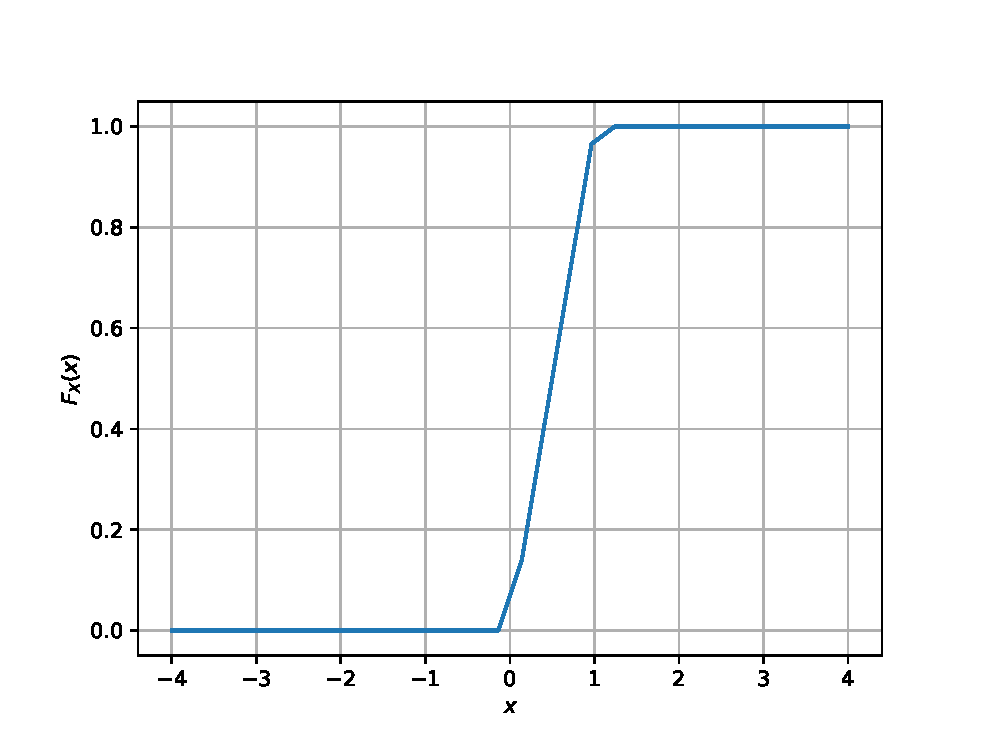
\includegraphics[width=\columnwidth]{./figs/uni_cdf}
\caption{The CDF of $U$}
\label{fig:uni_cdf}
\end{figure}

%
\item
Find a  theoretical expression for $F_{U}(x)$.

\item
The mean of $U$ is defined as
%
\begin{equation}
E\sbrak{U} = \frac{1}{N}\sum_{i=1}^{N}U_i
\end{equation}
%
and its variance as
%
\begin{equation}
\text{var}\sbrak{U} = E\sbrak{U- E\sbrak{U}}^2 
\end{equation}

Write a C program to  find the mean and variance of $U$. 
\item Verify your result theoretically given that
%
\begin{equation}
E\sbrak{U^k} = \int_{-\infty}^{\infty}x^kdF_{U}(x)
\end{equation}
\end{enumerate}
\section{Central Limit Theorem}
%
\begin{enumerate}[label=\thesection.\arabic*
,ref=\thesection.\theenumi]

%
\item
Generate $10^6$ samples of the random variable
%
\begin{equation}
X = \sum_{i=1}^{12}U_i -6
\end{equation}
%
using a C program, where $U_i, i = 1,2,\dots, 12$ are  a set of independent uniform random variables between 0 and 1
and save in a file called gau.dat

%
\item
Load gau.dat in python and plot the empirical CDF of $X$ using the samples in gau.dat. What properties does a CDF have?
\\
\solution The CDF of $X$ is plotted in Fig. \ref{fig:gauss_cdf}
\begin{figure}
\centering
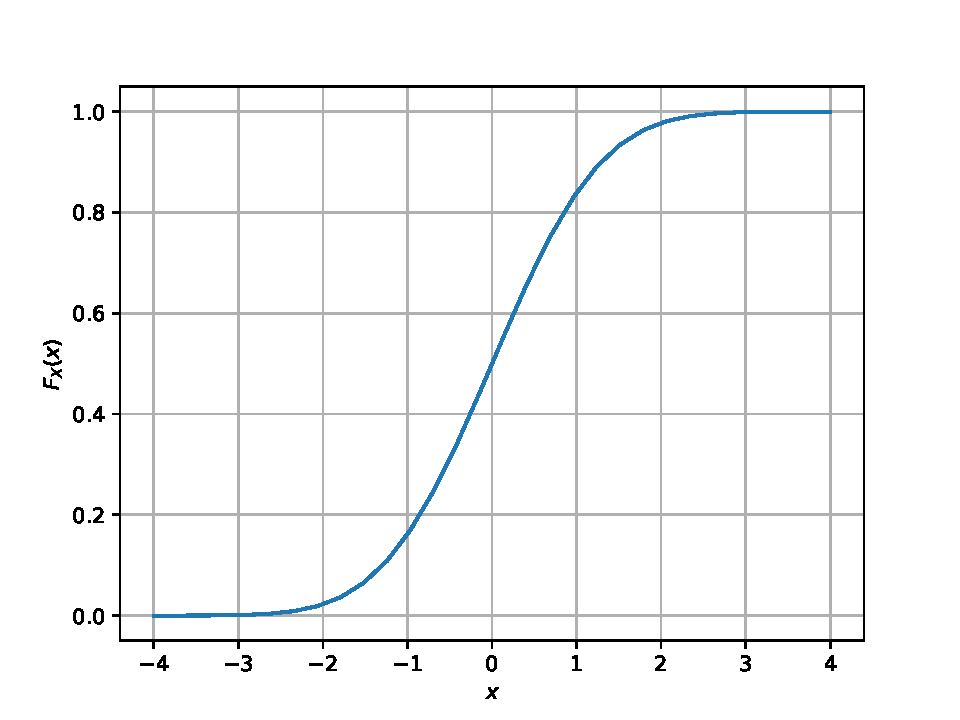
\includegraphics[width=\columnwidth]{./figs/gauss_cdf}
\caption{The CDF of $X$}
\label{fig:gauss_cdf}
\end{figure}
\item
Load gau.dat in python and plot the empirical PDF of $X$ using the samples in gau.dat. The PDF of $X$ is defined as
\begin{align}
p_{X}(x) = \frac{d}{dx}F_{X}(x)
\end{align}
What properties does the PDF have?
\\
\solution The PDF of $X$ is plotted in Fig. \ref{fig:gauss_pdf} using the code below
\begin{lstlisting}
codes/pdf_plot.py
\end{lstlisting}

\begin{figure}
\centering
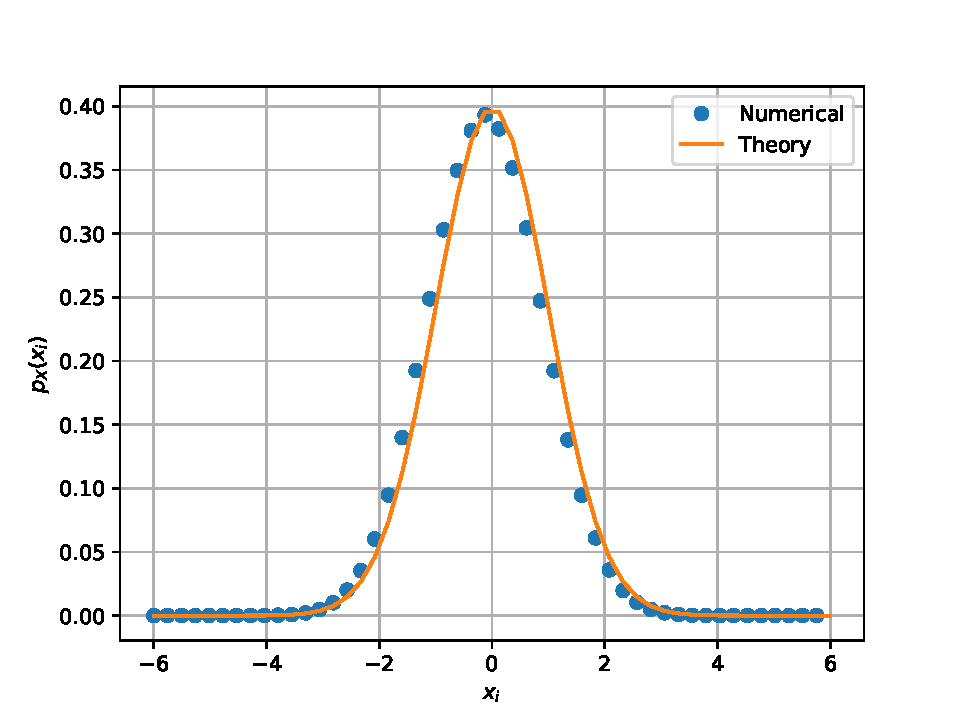
\includegraphics[width=\columnwidth]{./figs/gauss_pdf}
\caption{The PDF of $X$}
\label{fig:gauss_pdf}
\end{figure}

\item Find the mean and variance of $X$ by writing a C program.
\item Given that 
\begin{align}
p_{X}(x) = \frac{1}{\sqrt{2\pi}}\exp\brak{-\frac{x^2}{2}}, -\infty < x < \infty,
\end{align}
repeat the above exercise theoretically.
%
\end{enumerate}
\section{From Uniform to Other}
\begin{enumerate}[label=\thesection.\arabic*
,ref=\thesection.\theenumi]
%
\item
Generate samples of 
%
\begin{equation}
V = -2\ln\brak{1-U}
\end{equation}
%
and plot its CDF.  
\item Find a theoretical expression for $F_V(x)$.

%
%\item
%Generate the Rayleigh distribution from Uniform. Verify your result through graphical plots.
\end{enumerate}

\section{Triangular Distribution}
\begin{enumerate}[label=\thesection.\arabic*
,ref=\thesection.\theenumi]
%
\item Generate 
	\begin{align}
		T = U_1+U_2
	\end{align}
\item Find the CDF of $T$.
\item Find the PDF of $T$.
\item Find the theoretical expressions for the PDF and CDF of $T$.
\item Verify your results through a plot. 
\end{enumerate}
\iffalse
\section{Maximum Likelihood}
\begin{enumerate}[label=\thesection.\arabic*
,ref=\thesection.\theenumi]
\item Generate equiprobable $X \in \cbrak{1,-1}$.
\item Generate 
\begin{equation}
Y = AX+N,
\end{equation}
		where $A = 5$ dB,  and $N \sim \gauss{0}{1}$.
	\item Plot $Y$ using a scatter plot.
	\item Guess how to estimate $X$ from $Y$.
\item
\label{ml-ch4_sim}
Find 
\begin{equation}
	P_{e|0} = \pr{\hat{X} = -1|X=1}
\end{equation}
and 
\begin{equation}
	P_{e|1} = \pr{\hat{X} = 1|X=-1}
\end{equation}
%
\item Find $P_e$ assuming that $X$ has equiprobable symbols.

%
\item
Verify by plotting  the theoretical $P_e$ with respect to $A$ from 0 to 10 dB.  
%
\item Now, consider a threshold $\delta$  while estimating $X$ from $Y$. Find the value of $\delta$ that maximizes the theoretical $P_e$.
\item Repeat the above exercise when 
	\begin{align}
		p_{X}(0) = p
	\end{align}
\item Repeat the above exercise using the MAP criterion.

		\end{enumerate}
\section{Gaussian to Other}
\begin{enumerate}[label=\thesection.\arabic*
,ref=\thesection.\theenumi]
\item
Let $X_1 \sim  \gauss{0}{1}$ and $X_2 \sim  \gauss{0}{1}$. Plot the CDF and PDF of
%
\begin{equation}
V = X_1^2 + X_2^2
\end{equation}
%

%
%
\item
If
%
\begin{equation}
F_{V}(x) = 
\begin{cases}
1 - e^{-\alpha x} & x \geq 0 \\
0 & x < 0,
\end{cases}
\end{equation}
%
find $\alpha$.

%
\item
\label{ch3_raleigh_sim}
Plot the CDF and PDf of
%
\begin{equation}
A = \sqrt{V}
\end{equation}
%


\end{enumerate}

\section{Conditional Probability}
\begin{enumerate}[label=\thesection.\arabic*
,ref=\thesection.\theenumi]
\item
\label{ch4_sim}
Plot 
\begin{equation}
P_e = \pr{\hat{X} = -1|X=1}
\end{equation}
%
for 
\begin{equation}
Y = AX+N,
\end{equation}
where $A$ is Raleigh with $E\sbrak{A^2} = \gamma, N \sim \gauss{0}{1}, X \in \brak{-1,1}$ for $0 \le \gamma \le 10$ dB.

%
\item
Assuming that $N$ is a constant, find an expression for $P_e$.  Call this $P_e(N)$

%
\item
%
\label{ch4_anal}
For a function $g$,
\begin{equation}
E\sbrak{g(X)} = \int_{-\infty}^{\infty}g(x)p_{X}(x)\, dx
\end{equation}
%
Find $P_e = E\sbrak{P_e(N)}$.

%
\item
Plot $P_e$ in problems \ref{ch4_sim} and \ref{ch4_anal} on the same graph w.r.t $\gamma$.  Comment.

		\end{enumerate}
\section{Two Dimensions}
Let 
\begin{equation}
\mbf{y} = A\mbf{x} + \mbf{n},
\end{equation}
where 
\begin{align}
x &\in \brak{\mbf{s}_0,\mbf{s}_1}, 
\mbf{s}_0 = 
\begin{pmatrix}
1 
\\
0
\end{pmatrix},
\mbf{s}_1 = 
\begin{pmatrix}
0 
\\
1
\end{pmatrix}
\\
\mbf{n} &= 
\begin{pmatrix}
n_1
\\
n_2
\end{pmatrix},
n_1,n_2 \sim \gauss{0}{1}.
\end{align}
%
\begin{enumerate}[label=\thesection.\arabic*
,ref=\thesection.\theenumi]

%%
\item
\label{ch5_fsk}
Plot 
%
\begin{equation}
\mbf{y}|\mbf{s}_0 \text{ and } \mbf{y}|\mbf{s}_1
\end{equation}
%
on the same graph using a scatter plot.

%
\item
For the above problem, find a decision rule for detecting the symbols $\mbf{s}_0 $ and $\mbf{s}_1$.

%
\item
Plot 
\begin{equation} 
P_e = \pr{\hat{\mbf{x}} = \mbf{s}_1|\mbf{x} = \mbf{s}_0}
\end{equation}
with respect to the SNR from 0 to 10 dB.

%
\item
Obtain an expression for $P_e$. Verify this by comparing the theory and simulation plots on the same graph.

%
		\end{enumerate}
\end{document}
\fi

\chapter{Maximum Likelihood Detection: BPSK}
\iffalse
\let\negmedspace\undefined
\let\negthickspace\undefined
\documentclass[journal,12pt,twocolumn]{IEEEtran}
%\documentclass[conference]{IEEEtran}
%\IEEEoverridecommandlockouts
% The preceding line is only needed to identify funding in the first footnote. If that is unneeded, please comment it out.
\usepackage{cite}
\usepackage{amssymb,amsfonts,amsthm,amsmath}
\usepackage{algorithmic}
\usepackage{graphicx}
\usepackage{textcomp}
\usepackage{xcolor}
\usepackage{txfonts}
\usepackage{listings}
\usepackage{enumitem}
\usepackage{mathtools}
\usepackage{gensymb}

%%
%\usepackage{setspace}
%%\doublespacing
%\singlespacing
%
%%\usepackage{graphicx}
%%\usepackage{amssymb}
%%\usepackage{relsize}
%\usepackage[cmex10]{amsmath}
%%\interdisplaylinepenalty=2500
%%\savesymbol{iint}
%%\usepackage{txfonts}
%%\restoresymbol{TXF}{iint}
%%\usepackage{wasysym}
%\usepackage{amsthm}
%\usepackage{mathrsfs}
%\usepackage{txfonts}
%%\usepackage{stfloats}
%%\usepackage{cite}
%%\usepackage{cases}
%%\usepackage{subfig}
%%\usepackage{xtab}
%%\usepackage{multirow}
%%\usepackage{algorithm}
%%\usepackage{algpseudocode}
%%\usepackage{tikz}
%%\usepackage{circuitikz}
%%\usepackage{verbatim}
\usepackage{hyperref}
%%\usepackage{stmaryrd}
%%\usepackage{tkz-euclide} % loads  TikZ and tkz-base
%%\usetkzobj{all}
    \usepackage{color}                                            %%
    \usepackage{array}                                            %%
    \usepackage{longtable}                                        %%
    \usepackage{calc}                                             %%
    \usepackage{multirow}                                         %%
    \usepackage{hhline}                                           %%
    \usepackage{ifthen}                                           %%
%  %optionally (for landscape tables embedded in another document): %%
%    \usepackage{lscape}     
%%\usepackage{multicol}
%\usepackage{chngcntr}
%\usepackage{enumerate}

%\usepackage{wasysym}
%\newcounter{MYtempeqncnt}
\DeclareMathOperator*{\Res}{Res}
%\renewcommand{\baselinestretch}{2}
\renewcommand\thesection{\arabic{section}}
\renewcommand\thesubsection{\thesection.\arabic{subsection}}
\renewcommand\thesubsubsection{\thesubsection.\arabic{subsubsection}}

\renewcommand\thesectiondis{\arabic{section}}
\renewcommand\thesubsectiondis{\thesectiondis.\arabic{subsection}}
\renewcommand\thesubsubsectiondis{\thesubsectiondis.\arabic{subsubsection}}

% correct bad hyphenation here
\hyphenation{op-tical net-works semi-conduc-tor}
\def\inputGnumericTable{}                                 %%

\lstset{
language=tex,
frame=single, 
breaklines=true
}

\begin{document}
%


\newtheorem{theorem}{Theorem}[section]
\newtheorem{problem}{Problem}
\newtheorem{proposition}{Proposition}[section]
\newtheorem{lemma}{Lemma}[section]
\newtheorem{corollary}[theorem]{Corollary}
\newtheorem{example}{Example}[section]
\newtheorem{definition}[problem]{Definition}
%\newtheorem{thm}{Theorem}[section] 
%\newtheorem{defn}[thm]{Definition}
%\newtheorem{algorithm}{Algorithm}[section]
%\newtheorem{cor}{Corollary}
\newcommand{\BEQA}{\begin{eqnarray}}
\newcommand{\EEQA}{\end{eqnarray}}
\newcommand{\define}{\stackrel{\triangle}{=}}

\bibliographystyle{IEEEtran}
%\bibliographystyle{ieeetr}


\providecommand{\mbf}{\mathbf}
\providecommand{\pr}[1]{\ensuremath{\Pr\left(#1\right)}}
\providecommand{\re}[1]{\ensuremath{\text{Re}\left(#1\right)}}
\providecommand{\im}[1]{\ensuremath{\text{Im}\left(#1\right)}}
\providecommand{\qfunc}[1]{\ensuremath{Q\left(#1\right)}}
\providecommand{\sbrak}[1]{\ensuremath{{}\left[#1\right]}}
\providecommand{\lsbrak}[1]{\ensuremath{{}\left[#1\right.}}
\providecommand{\rsbrak}[1]{\ensuremath{{}\left.#1\right]}}
\providecommand{\brak}[1]{\ensuremath{\left(#1\right)}}
\providecommand{\lbrak}[1]{\ensuremath{\left(#1\right.}}
\providecommand{\rbrak}[1]{\ensuremath{\left.#1\right)}}
\providecommand{\cbrak}[1]{\ensuremath{\left\{#1\right\}}}
\providecommand{\lcbrak}[1]{\ensuremath{\left\{#1\right.}}
\providecommand{\rcbrak}[1]{\ensuremath{\left.#1\right\}}}
\theoremstyle{remark}
\newtheorem{rem}{Remark}
\newcommand{\sgn}{\mathop{\mathrm{sgn}}}
\providecommand{\abs}[1]{\left\vert#1\right\vert}
\providecommand{\res}[1]{\Res\displaylimits_{#1}} 
\providecommand{\norm}[1]{\left\lVert#1\right\rVert}
%\providecommand{\norm}[1]{\lVert#1\rVert}
\providecommand{\mtx}[1]{\mathbf{#1}}
\providecommand{\mean}[1]{E\left[ #1 \right]}
\providecommand{\fourier}{\overset{\mathcal{F}}{ \rightleftharpoons}}
%\providecommand{\hilbert}{\overset{\mathcal{H}}{ \rightleftharpoons}}
\providecommand{\system}{\overset{\mathcal{H}}{ \longleftrightarrow}}
	%\newcommand{\solution}[2]{\textbf{Solution:}{#1}}
\newcommand{\solution}{\noindent \textbf{Solution: }}
\providecommand{\dec}[2]{\ensuremath{\overset{#1}{\underset{#2}{\gtrless}}}}
\newcommand{\myvec}[1]{\ensuremath{\begin{pmatrix}#1\end{pmatrix}}}
\newcommand{\mydet}[1]{\ensuremath{\begin{vmatrix}#1\end{vmatrix}}}
	\newcommand*{\permcomb}[4][0mu]{{{}^{#3}\mkern#1#2_{#4}}}
\newcommand*{\perm}[1][-3mu]{\permcomb[#1]{P}}
\newcommand*{\comb}[1][-1mu]{\permcomb[#1]{C}}
\providecommand{\gauss}[2]{\mathcal{N}\ensuremath{\left(#1,#2\right)}}
%%
%	%\newcommand{\solution}[2]{\textbf{Solution:}{#1}}
%\newcommand{\solution}{\noindent \textbf{Solution: }}
\newcommand{\cosec}{\,\text{cosec}\,}
\newcommand{\sinc}{\,\text{sinc}\,}
\newcommand{\rect}{\,\text{rect}\,}

%\numberwithin{equation}{section}
\numberwithin{equation}{subsection}
%\numberwithin{problem}{section}
%\numberwithin{definition}{section}
\makeatletter
\@addtoreset{figure}{problem}
\makeatother

\let\StandardTheFigure\thefigure
\let\vec\mathbf
\let\j\jmath
%\renewcommand{\thefigure}{\theproblem.\arabic{figure}}
\renewcommand{\thefigure}{\theproblem}
%\setlist[enumerate,1]{before=\renewcommand\theequation{\theenumi.\arabic{equation}}
%\counterwithin{equation}{enumi}


%\renewcommand{\theequation}{\arabic{subsection}.\arabic{equation}}

\def\putbox#1#2#3{\makebox[0in][l]{\makebox[#1][l]{}\raisebox{\baselineskip}[0in][0in]{\raisebox{#2}[0in][0in]{#3}}}}
     \def\rightbox#1{\makebox[0in][r]{#1}}
     \def\centbox#1{\makebox[0in]{#1}}
     \def\topbox#1{\raisebox{-\baselineskip}[0in][0in]{#1}}
     \def\midbox#1{\raisebox{-0.5\baselineskip}[0in][0in]{#1}}

\vspace{3cm}

\title{
%	\logo{
	Probability
%	}
}
%\title{
%	\logo{Matrix Analysis through Octave}{\begin{center}\includegraphics[scale=.24]{tlc}\end{center}}{}{HAMDSP}
%}


% paper title
% can use linebreaks \\ within to get better formatting as desired
%\title{Matrix Analysis through Octave}
%
%
% author names and IEEE memberships
% note positions of commas and nonbreaking spaces ( ~ ) LaTeX will not break
% a structure at a ~ so this keeps an author's name from being broken across
% two lines.
% use \thanks{} to gain access to the first footnote area
% a separate \thanks must be used for each paragraph as LaTeX2e's \thanks
% was not built to handle multiple paragraphs
%

\author{
	G. V. V. Sharma
	%<-this % stops a space
%\thanks{}}
}
% note the % following the last \IEEEmembership and also \thanks - 
% these prevent an unwanted space from occurring between the last author name
% and the end of the author line. i.e., if you had this:
% 
% \author{....lastname \thanks{...} \thanks{...} }
%                     ^------------^------------^----Do not want these spaces!
%
% a space would be appended to the last name and could cause every name on that
% line to be shifted left slightly. This is one of those "LaTeX things". For
% instance, "\textbf{A} \textbf{B}" will typeset as "A B" not "AB". To get
% "AB" then you have to do: "\textbf{A}\textbf{B}"
% \thanks is no different in this regard, so shield the last } of each \thanks
% that ends a line with a % and do not let a space in before the next \thanks.
% Spaces after \IEEEmembership other than the last one are OK (and needed) as
% you are supposed to have spaces between the names. For what it is worth,
% this is a minor point as most people would not even notice if the said evil
% space somehow managed to creep in.



% The paper headers
%\markboth{Journal of \LaTeX\ Class Files,~Vol.~6, No.~1, January~2007}%
%{Shell \MakeLowercase{\textit{et al.}}: Bare Demo of IEEEtran.cls for Journals}
% The only time the second header will appear is for the odd numbered pages
% after the title page when using the twoside option.
% 
% *** Note that you probably will NOT want to include the author's ***
% *** name in the headers of peer review papers.                   ***
% You can use \ifCLASSOPTIONpeerreview for conditional compilation here if
% you desire.




% If you want to put a publisher's ID mark on the page you can do it like
% this:
%\IEEEpubid{0000--0000/00\$00.00~\copyright~2007 IEEE}
% Remember, if you use this you must call \IEEEpubidadjcol in the second
% column for its text to clear the IEEEpubid mark.



% make the title area
\maketitle

\newpage

\tableofcontents

\bigskip

\renewcommand{\thefigure}{\theenumi}
\renewcommand{\thetable}{\theenumi}
%\renewcommand{\theequation}{\theenumi}

%\begin{abstract}
%%\boldmath
%In this letter, an algorithm for evaluating the exact analytical bit error rate  (BER)  for the piecewise linear (PL) combiner for  multiple relays is presented. Previous results were available only for upto three relays. The algorithm is unique in the sense that  the actual mathematical expressions, that are prohibitively large, need not be explicitly obtained. The diversity gain due to multiple relays is shown through plots of the analytical BER, well supported by simulations. 
%
%\end{abstract}
% IEEEtran.cls defaults to using nonbold math in the Abstract.
% This preserves the distinction between vectors and scalars. However,
% if the journal you are submitting to favors bold math in the abstract,
% then you can use LaTeX's standard command \boldmath at the very start
% of the abstract to achieve this. Many IEEE journals frown on math
% in the abstract anyway.

% Note that keywords are not normally used for peerreview papers.
%\begin{IEEEkeywords}
%Cooperative diversity, decode and forward, piecewise linear
%\end{IEEEkeywords}



% For peer review papers, you can put extra information on the cover
% page as needed:
% \ifCLASSOPTIONpeerreview
% \begin{center} \bfseries EDICS Category: 3-BBND \end{center}
% \fi
%
% For peerreview papers, this IEEEtran command inserts a page break and
% creates the second title. It will be ignored for other modes.
%\IEEEpeerreviewmaketitle

%\begin{abstract}
%\end{abstract}

%\iffalse





%% Copyright (C) 2020 Saurabh Joshi
%%% 
%\let\negmedspace\undefined
%\let\negthickspace\undefined
%
%\documentclass[journal,12pt,onecolumn]{IEEEtran}
%%\documentclass[journal,12pt,twocolumn]{IEEEtran}
%%
%\usepackage{setspace}
%\usepackage{gensymb}
%%\doublespacing
%\singlespacing
%
%%\usepackage{graphicx}
%%\usepackage{amssymb}
%%\usepackage{relsize}
%\usepackage[cmex10]{amsmath}
%%\usepackage{amsthm}
%%\interdisplaylinepenalty=2500
%%\savesymbol{iint}
%%\usepackage{txfonts}
%%\restoresymbol{TXF}{iint}
%%\usepackage{wasysym}
%\usepackage{amsthm}
%\usepackage{mathrsfs}
%\usepackage{txfonts}
%\usepackage{stfloats}
%\usepackage{cite}
%\usepackage{cases}
%\usepackage{subfig}
%%\usepackage{xtab}
%\usepackage{longtable}
%\usepackage{multirow}
%%\usepackage{algorithm}
%%\usepackage{algpseudocode}
%\usepackage{enumitem}
%\usepackage{mathtools}
%\usepackage{tikz}
%\usepackage{circuitikz}
%\usepackage{verbatim}
%\usepackage{hyperref}
%%\usepackage{stmaryrd}
%\usepackage{tkz-euclide} % loads  TikZ and tkz-base
%%\usetkzobj{all}
%\usepackage{listings}
%    \usepackage{color}                                            %%
%    \usepackage{array}                                            %%
%    \usepackage{longtable}                                        %%
%    \usepackage{calc}                                             %%
%    \usepackage{multirow}                                         %%
%    \usepackage{hhline}                                           %%
%    \usepackage{ifthen}                                           %%
%  %optionally (for landscape tables embedded in another document): %%
%    \usepackage{lscape}     
%\usepackage{multicol}
%\usepackage{chngcntr}
%\usepackage{iftex}
%%\usepackage[latin9]{inputenc}
%\usepackage{geometry}
%\usepackage{bm}
%%\geometry{verbose,tmargin=2cm,bmargin=3cm,lmargin=1.8cm,rmargin=1.5cm,headheight=2cm,headsep=2cm,footskip=3cm}
%\usepackage{array}
%\newcolumntype{L}[1]{>{\raggedright\let\newline\\\arraybackslash\hspace{0pt}}m{#1}}
%\newcolumntype{C}[1]{>{\centering\let\newline\\\arraybackslash\hspace{0pt}}m{#1}}
%\newcolumntype{R}[1]{>{\raggedleft\let\newline\\\arraybackslash\hspace{0pt}}m{#1}}
%
%%\usepackage{graphicx}
%%\usepackage{setspace}
%%\usepackage{parskip}
%
%\def \hsp {\hspace{3mm}}
%
%\makeatletter
%
%\providecommand{\tabularnewline}{\\}
%
%
%
%\makeatother
%\ifxetex
%\usepackage[T1]{fontenc}
%\usepackage{fontspec}
%%\setmainfont[ Path = fonts/]{Sanskrit_2003.ttf}
%\newfontfamily\nakulafont[Script=Devanagari,AutoFakeBold=2,Path = fonts/]{Nakula}
%%\newfontfamily\liberationfont{Liberation Sans Narrow}
%%\newfontfamily\liberationsansfont{Liberation Sans}
%\fi
%\usepackage{tikz}
%\usepackage{xcolor}
%%\usepackage{enumerate}
%
%%\usepackage{wasysym}
%%\newcounter{MYtempeqncnt}
%\DeclareMathOperator*{\Res}{Res}
%%\renewcommand{\baselinestretch}{2}
%\renewcommand\thesection{\arabic{section}}
%\renewcommand\thesubsection{\thesection.\arabic{subsection}}
%\renewcommand\thesubsubsection{\thesubsection.\arabic{subsubsection}}
%
%\renewcommand\thesectiondis{\arabic{section}}
%\renewcommand\thesubsectiondis{\thesectiondis.\arabic{subsection}}
%\renewcommand\thesubsubsectiondis{\thesubsectiondis.\arabic{subsubsection}}
%
%% correct bad hyphenation here
%\hyphenation{op-tical net-works semi-conduc-tor}
%\def\inputGnumericTable{}                                 %%
%
%\lstset{
%language=tex,
%frame=single, 
%breaklines=true
%}
%
%%\begin{document}
%%
%
%
%\newtheorem{theorem}{Theorem}[section]
%\newtheorem{problem}{Problem}
%\newtheorem{proposition}{Proposition}[section]
%\newtheorem{lemma}{Lemma}[section]
%\newtheorem{corollary}[theorem]{Corollary}
%\newtheorem{example}{Example}[section]
%\newtheorem{definition}[problem]{Definition}
%%\newtheorem{thm}{Theorem}[section] 
%%\newtheorem{defn}[thm]{Definition}
%%\newtheorem{algorithm}{Algorithm}[section]
%%\newtheorem{cor}{Corollary}
%\newcommand{\BEQA}{\begin{eqnarray}}
%\newcommand{\EEQA}{\end{eqnarray}}
%\newcommand{\define}{\stackrel{\triangle}{=}}
%
%\bibliographystyle{IEEEtran}
%%\bibliographystyle{ieeetr}
%
%
%\providecommand{\mbf}{\mathbf}
%\providecommand{\pr}[1]{\ensuremath{\Pr\left(#1\right)}}
%\providecommand{\qfunc}[1]{\ensuremath{Q\left(#1\right)}}
%\providecommand{\sbrak}[1]{\ensuremath{{}\left[#1\right]}}
%\providecommand{\lsbrak}[1]{\ensuremath{{}\left[#1\right.}}
%\providecommand{\rsbrak}[1]{\ensuremath{{}\left.#1\right]}}
%\providecommand{\brak}[1]{\ensuremath{\left(#1\right)}}
%\providecommand{\lbrak}[1]{\ensuremath{\left(#1\right.}}
%\providecommand{\rbrak}[1]{\ensuremath{\left.#1\right)}}
%\providecommand{\cbrak}[1]{\ensuremath{\left\{#1\right\}}}
%\providecommand{\lcbrak}[1]{\ensuremath{\left\{#1\right.}}
%\providecommand{\rcbrak}[1]{\ensuremath{\left.#1\right\}}}
%\theoremstyle{remark}
%\newtheorem{rem}{Remark}
%\newcommand{\sgn}{\mathop{\mathrm{sgn}}}
%\providecommand{\abs}[1]{\left\vert#1\right\vert}
%\providecommand{\res}[1]{\Res\displaylimits_{#1}} 
%\providecommand{\norm}[1]{\left\lVert#1\right\rVert}
%%\providecommand{\norm}[1]{\lVert#1\rVert}
%\providecommand{\mtx}[1]{\mathbf{#1}}
%\providecommand{\mean}[1]{E\left[ #1 \right]}
%%\numberwithin{equation}{section}
%\numberwithin{equation}{section}
%%\numberwithin{problem}{section}
%%\numberwithin{definition}{section}
%\makeatletter
%\@addtoreset{figure}{problem}
%\makeatother
%
%\let\StandardTheFigure\thefigure
%\let\vec\mathbf
%%\renewcommand{\thefigure}{\theproblem.\arabic{figure}}
%\renewcommand{\thefigure}{\theproblem}
%%\setlist[enumerate,1]{before=\renewcommand\theequation{\theenumi.\arabic{equation}}
%%\counterwithin{equation}{enumi}
%
%
%%\renewcommand{\theequation}{\arabic{subsection}.\arabic{equation}}
%
%\vspace{3cm}
%
%
%%\usepackage{babel}
%\begin{document}
%
%\begin{tabular}{L{6cm} C{5cm} R{5cm} }
%
%	\definecolor{circleorange}{rgb}{1,0.17,0.08}
%\definecolor{darkorange}{rgb}{1,0.27,0.1}
%\definecolor{orange2}{rgb}{1,0.5,0.15}
%\definecolor{orange3}{rgb}{1,0.65,0.25}
%\definecolor{yellow1}{rgb}{0.95,0.77,0.2}
%%\begin{tikzpicture}[scale=0.2,every node/.style={transform shape}]
%\begin{tikzpicture}[scale=0.1,every node/.style={transform shape}]
%\draw [fill=circleorange,circleorange] (5,10) circle (1.15); 
%\fill [darkorange] (5.06,8) -- (5.06,2) -- (7.3,1.2) -- (7.3,8.8) -- (5.06,8);
%\fill [darkorange] (4.94,8) -- (4.94,2) -- (2.7,1.2) -- (2.7,8.8) -- (4.94,8);
%\fill [orange2]    (7.4,8.4) -- (7.4,1.6) -- (8.2,1.2) -- (8.2,8.8) -- (7.4,8.4);
%\fill [orange2]    (2.6,8.4) -- (2.6,1.6) -- (1.8,1.2) -- (1.8,8.8) -- (2.6,8.4);
%\fill [orange3]    (8.3,8.4) -- (8.3,1.6) -- (9.0,1.2) -- (9.0,8.8) -- (8.3,8.4);
%\fill [orange3]    (1.7,8.4) -- (1.7,1.6) -- (1.0,1.2) -- (1.0,8.8) -- (1.7,8.4);
%\fill [yellow1]    (9.1,8.4) -- (9.1,1.6) -- (9.7,1.2) -- (9.7,8.8) -- (9.1,8.4);
%\fill [yellow1]    (0.9,8.4) -- (0.9,1.6) -- (0.3,1.2) -- (0.3,8.8) -- (0.9,8.4);
%\ifxetex
%\node [scale=2.1] at (5,-0.1)  {   {\bf {\nakulafont  भारतीय प्रौद्योगिकी संस्थान हैदराबाद }} };
%\node [scale=1.8] at (5,-1.2) {   {\bf { Indian Institute of Technology Hyderabad}} };
%%\node [scale=1.8] at (5,-1.2) {   {\bf {\liberationsansfont Indian Institute of Technology Hyderabad}} };
%\fi
%\end{tikzpicture}
%% \includegraphics[scale=0.05]{logo_iith} \newline
%
%& Assignments 
%	&
%	AI1110
%\end{tabular}
%
%
%\vspace{-6mm}
%\begin{center}
%%\includegraphics[scale=0.95]{Yellow-Line}
%\begin{tikzpicture}
%\definecolor{yellow1}{rgb}{0.95,0.77,0.2}
%\draw[line width=0.75mm, yellow1] (0,0) -- (\textwidth,0);
%\end{tikzpicture}
%\par\end{center}
		\numberwithin{equation}{enumi}
\section{Uniform Random Numbers}
Let $U$ be a uniform random variable between 0 and 1.
\begin{enumerate}[label=\thesection.\arabic*
,ref=\thesection.\theenumi]
\item Generate $10^6$ samples of $U$ using a C program and save into a file called uni.dat .
\\
\solution Download the following files and execute the  C program.
\begin{lstlisting}
codes/exrand.c
codes/coeffs.h
\end{lstlisting}

%
\item
Load the uni.dat file into python and plot the empirical CDF of $U$ using the samples in uni.dat. The CDF is defined as
\begin{align}
F_{U}(x) = \pr{U \le x}
\end{align}
\\
\solution  The following code plots Fig. \ref{fig:uni_cdf}
\begin{lstlisting}
codes/cdf_plot.py
\end{lstlisting}
\begin{figure}
\centering
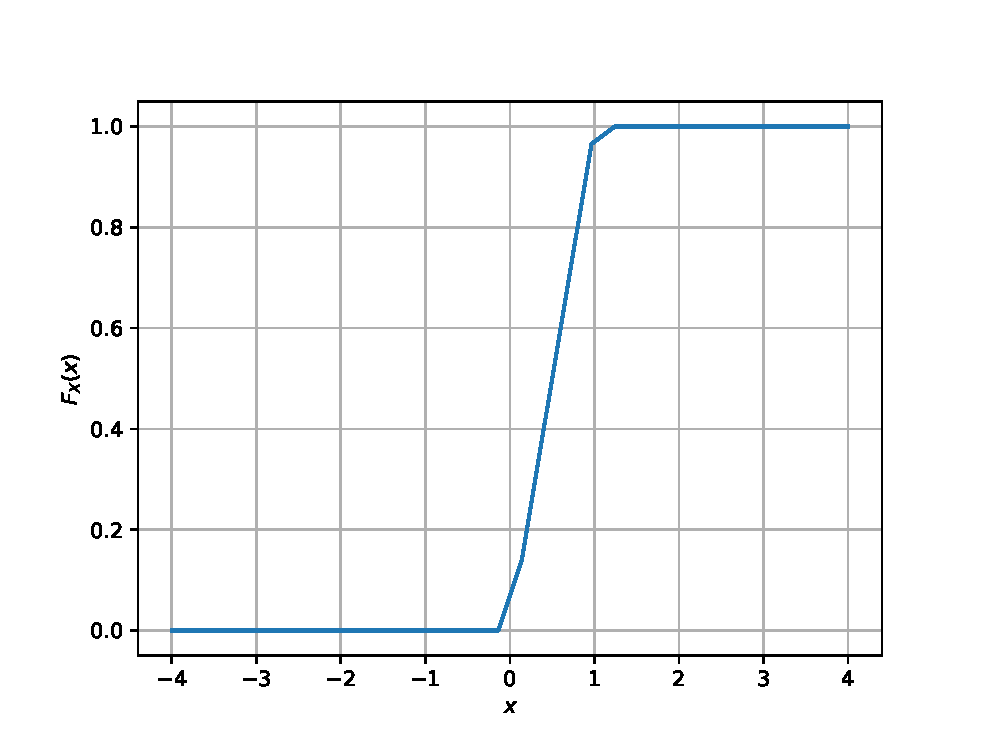
\includegraphics[width=\columnwidth]{./figs/uni_cdf}
\caption{The CDF of $U$}
\label{fig:uni_cdf}
\end{figure}

%
\item
Find a  theoretical expression for $F_{U}(x)$.

\item
The mean of $U$ is defined as
%
\begin{equation}
E\sbrak{U} = \frac{1}{N}\sum_{i=1}^{N}U_i
\end{equation}
%
and its variance as
%
\begin{equation}
\text{var}\sbrak{U} = E\sbrak{U- E\sbrak{U}}^2 
\end{equation}

Write a C program to  find the mean and variance of $U$. 
\item Verify your result theoretically given that
%
\begin{equation}
E\sbrak{U^k} = \int_{-\infty}^{\infty}x^kdF_{U}(x)
\end{equation}
\end{enumerate}
\section{Central Limit Theorem}
%
\begin{enumerate}[label=\thesection.\arabic*
,ref=\thesection.\theenumi]

%
\item
Generate $10^6$ samples of the random variable
%
\begin{equation}
X = \sum_{i=1}^{12}U_i -6
\end{equation}
%
using a C program, where $U_i, i = 1,2,\dots, 12$ are  a set of independent uniform random variables between 0 and 1
and save in a file called gau.dat

%
\item
Load gau.dat in python and plot the empirical CDF of $X$ using the samples in gau.dat. What properties does a CDF have?
\\
\solution The CDF of $X$ is plotted in Fig. \ref{fig:gauss_cdf}
\begin{figure}
\centering
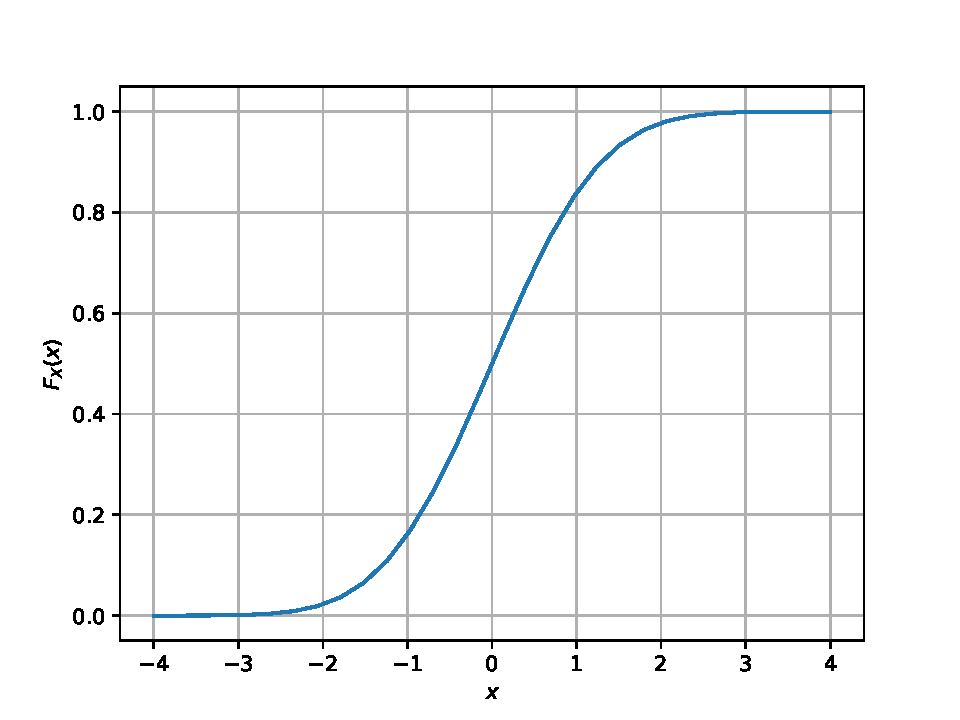
\includegraphics[width=\columnwidth]{./figs/gauss_cdf}
\caption{The CDF of $X$}
\label{fig:gauss_cdf}
\end{figure}
\item
Load gau.dat in python and plot the empirical PDF of $X$ using the samples in gau.dat. The PDF of $X$ is defined as
\begin{align}
p_{X}(x) = \frac{d}{dx}F_{X}(x)
\end{align}
What properties does the PDF have?
\\
\solution The PDF of $X$ is plotted in Fig. \ref{fig:gauss_pdf} using the code below
\begin{lstlisting}
codes/pdf_plot.py
\end{lstlisting}

\begin{figure}
\centering
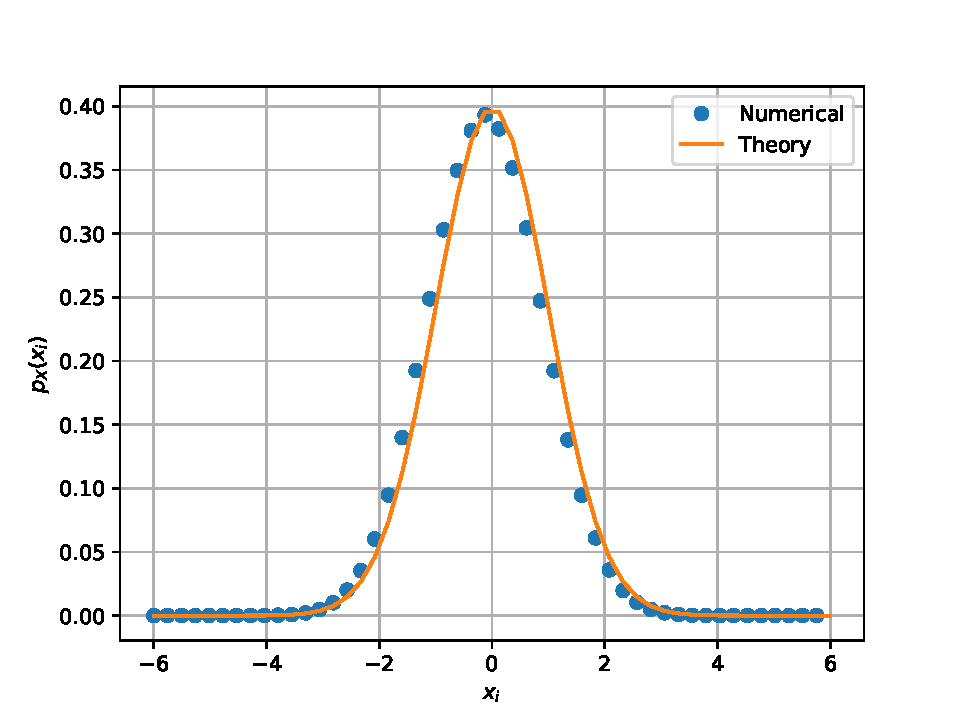
\includegraphics[width=\columnwidth]{./figs/gauss_pdf}
\caption{The PDF of $X$}
\label{fig:gauss_pdf}
\end{figure}

\item Find the mean and variance of $X$ by writing a C program.
\item Given that 
\begin{align}
p_{X}(x) = \frac{1}{\sqrt{2\pi}}\exp\brak{-\frac{x^2}{2}}, -\infty < x < \infty,
\end{align}
repeat the above exercise theoretically.
%
\end{enumerate}
\section{From Uniform to Other}
\begin{enumerate}[label=\thesection.\arabic*
,ref=\thesection.\theenumi]
%
\item
Generate samples of 
%
\begin{equation}
V = -2\ln\brak{1-U}
\end{equation}
%
and plot its CDF.  
\item Find a theoretical expression for $F_V(x)$.

%
%\item
%Generate the Rayleigh distribution from Uniform. Verify your result through graphical plots.
\end{enumerate}

\section{Triangular Distribution}
\begin{enumerate}[label=\thesection.\arabic*
,ref=\thesection.\theenumi]
%
\item Generate 
	\begin{align}
		T = U_1+U_2
	\end{align}
\item Find the CDF of $T$.
\item Find the PDF of $T$.
\item Find the theoretical expressions for the PDF and CDF of $T$.
\item Verify your results through a plot. 
\end{enumerate}
		\fi
\section{Maximum Likelihood}
\begin{enumerate}[label=\thesection.\arabic*
,ref=\thesection.\theenumi]
\item Generate equiprobable $X \in \cbrak{1,-1}$.
\item Generate 
\begin{equation}
Y = AX+N,
\end{equation}
		where $A = 5$ dB,  and $N \sim \gauss{0}{1}$.
	\item Plot $Y$ using a scatter plot.
	\item Guess how to estimate $X$ from $Y$.
\item
\label{ml-ch4_sim}
Find 
\begin{equation}
	P_{e|0} = \pr{\hat{X} = -1|X=1}
\end{equation}
and 
\begin{equation}
	P_{e|1} = \pr{\hat{X} = 1|X=-1}
\end{equation}
%
\item Find $P_e$ assuming that $X$ has equiprobable symbols.

%
\item
Verify by plotting  the theoretical $P_e$ with respect to $A$ from 0 to 10 dB.  
%
\item Now, consider a threshold $\delta$  while estimating $X$ from $Y$. Find the value of $\delta$ that maximizes the theoretical $P_e$.
\item Repeat the above exercise when 
	\begin{align}
		p_{X}(0) = p
	\end{align}
\item Repeat the above exercise using the MAP criterion.

		\end{enumerate}
		\iffalse
\section{Gaussian to Other}
\begin{enumerate}[label=\thesection.\arabic*
,ref=\thesection.\theenumi]
\item
Let $X_1 \sim  \gauss{0}{1}$ and $X_2 \sim  \gauss{0}{1}$. Plot the CDF and PDF of
%
\begin{equation}
V = X_1^2 + X_2^2
\end{equation}
%

%
%
\item
If
%
\begin{equation}
F_{V}(x) = 
\begin{cases}
1 - e^{-\alpha x} & x \geq 0 \\
0 & x < 0,
\end{cases}
\end{equation}
%
find $\alpha$.

%
\item
\label{ch3_raleigh_sim}
Plot the CDF and PDf of
%
\begin{equation}
A = \sqrt{V}
\end{equation}
%


\end{enumerate}

\section{Conditional Probability}
\begin{enumerate}[label=\thesection.\arabic*
,ref=\thesection.\theenumi]
\item
\label{ch4_sim}
Plot 
\begin{equation}
P_e = \pr{\hat{X} = -1|X=1}
\end{equation}
%
for 
\begin{equation}
Y = AX+N,
\end{equation}
where $A$ is Raleigh with $E\sbrak{A^2} = \gamma, N \sim \gauss{0}{1}, X \in \brak{-1,1}$ for $0 \le \gamma \le 10$ dB.

%
\item
Assuming that $N$ is a constant, find an expression for $P_e$.  Call this $P_e(N)$

%
\item
%
\label{ch4_anal}
For a function $g$,
\begin{equation}
E\sbrak{g(X)} = \int_{-\infty}^{\infty}g(x)p_{X}(x)\, dx
\end{equation}
%
Find $P_e = E\sbrak{P_e(N)}$.

%
\item
Plot $P_e$ in problems \ref{ch4_sim} and \ref{ch4_anal} on the same graph w.r.t $\gamma$.  Comment.

		\end{enumerate}
\section{Two Dimensions}
Let 
\begin{equation}
\mbf{y} = A\mbf{x} + \mbf{n},
\end{equation}
where 
\begin{align}
x &\in \brak{\mbf{s}_0,\mbf{s}_1}, 
\mbf{s}_0 = 
\begin{pmatrix}
1 
\\
0
\end{pmatrix},
\mbf{s}_1 = 
\begin{pmatrix}
0 
\\
1
\end{pmatrix}
\\
\mbf{n} &= 
\begin{pmatrix}
n_1
\\
n_2
\end{pmatrix},
n_1,n_2 \sim \gauss{0}{1}.
\end{align}
%
\begin{enumerate}[label=\thesection.\arabic*
,ref=\thesection.\theenumi]

%%
\item
\label{ch5_fsk}
Plot 
%
\begin{equation}
\mbf{y}|\mbf{s}_0 \text{ and } \mbf{y}|\mbf{s}_1
\end{equation}
%
on the same graph using a scatter plot.

%
\item
For the above problem, find a decision rule for detecting the symbols $\mbf{s}_0 $ and $\mbf{s}_1$.

%
\item
Plot 
\begin{equation} 
P_e = \pr{\hat{\mbf{x}} = \mbf{s}_1|\mbf{x} = \mbf{s}_0}
\end{equation}
with respect to the SNR from 0 to 10 dB.

%
\item
Obtain an expression for $P_e$. Verify this by comparing the theory and simulation plots on the same graph.

%
		\end{enumerate}
\end{document}
\fi

\chapter{Transformation of Random Variables}
\iffalse
\let\negmedspace\undefined
\let\negthickspace\undefined
\documentclass[journal,12pt,twocolumn]{IEEEtran}
%\documentclass[conference]{IEEEtran}
%\IEEEoverridecommandlockouts
% The preceding line is only needed to identify funding in the first footnote. If that is unneeded, please comment it out.
\usepackage{cite}
\usepackage{amssymb,amsfonts,amsthm,amsmath}
\usepackage{algorithmic}
\usepackage{graphicx}
\usepackage{textcomp}
\usepackage{xcolor}
\usepackage{txfonts}
\usepackage{listings}
\usepackage{enumitem}
\usepackage{mathtools}
\usepackage{gensymb}

%%
%\usepackage{setspace}
%%\doublespacing
%\singlespacing
%
%%\usepackage{graphicx}
%%\usepackage{amssymb}
%%\usepackage{relsize}
%\usepackage[cmex10]{amsmath}
%%\interdisplaylinepenalty=2500
%%\savesymbol{iint}
%%\usepackage{txfonts}
%%\restoresymbol{TXF}{iint}
%%\usepackage{wasysym}
%\usepackage{amsthm}
%\usepackage{mathrsfs}
%\usepackage{txfonts}
%%\usepackage{stfloats}
%%\usepackage{cite}
%%\usepackage{cases}
%%\usepackage{subfig}
%%\usepackage{xtab}
%%\usepackage{multirow}
%%\usepackage{algorithm}
%%\usepackage{algpseudocode}
%%\usepackage{tikz}
%%\usepackage{circuitikz}
%%\usepackage{verbatim}
\usepackage{hyperref}
%%\usepackage{stmaryrd}
%%\usepackage{tkz-euclide} % loads  TikZ and tkz-base
%%\usetkzobj{all}
    \usepackage{color}                                            %%
    \usepackage{array}                                            %%
    \usepackage{longtable}                                        %%
    \usepackage{calc}                                             %%
    \usepackage{multirow}                                         %%
    \usepackage{hhline}                                           %%
    \usepackage{ifthen}                                           %%
%  %optionally (for landscape tables embedded in another document): %%
%    \usepackage{lscape}     
%%\usepackage{multicol}
%\usepackage{chngcntr}
%\usepackage{enumerate}

%\usepackage{wasysym}
%\newcounter{MYtempeqncnt}
\DeclareMathOperator*{\Res}{Res}
%\renewcommand{\baselinestretch}{2}
\renewcommand\thesection{\arabic{section}}
\renewcommand\thesubsection{\thesection.\arabic{subsection}}
\renewcommand\thesubsubsection{\thesubsection.\arabic{subsubsection}}

\renewcommand\thesectiondis{\arabic{section}}
\renewcommand\thesubsectiondis{\thesectiondis.\arabic{subsection}}
\renewcommand\thesubsubsectiondis{\thesubsectiondis.\arabic{subsubsection}}

% correct bad hyphenation here
\hyphenation{op-tical net-works semi-conduc-tor}
\def\inputGnumericTable{}                                 %%

\lstset{
language=tex,
frame=single, 
breaklines=true
}

\begin{document}
%


\newtheorem{theorem}{Theorem}[section]
\newtheorem{problem}{Problem}
\newtheorem{proposition}{Proposition}[section]
\newtheorem{lemma}{Lemma}[section]
\newtheorem{corollary}[theorem]{Corollary}
\newtheorem{example}{Example}[section]
\newtheorem{definition}[problem]{Definition}
%\newtheorem{thm}{Theorem}[section] 
%\newtheorem{defn}[thm]{Definition}
%\newtheorem{algorithm}{Algorithm}[section]
%\newtheorem{cor}{Corollary}
\newcommand{\BEQA}{\begin{eqnarray}}
\newcommand{\EEQA}{\end{eqnarray}}
\newcommand{\define}{\stackrel{\triangle}{=}}

\bibliographystyle{IEEEtran}
%\bibliographystyle{ieeetr}


\providecommand{\mbf}{\mathbf}
\providecommand{\pr}[1]{\ensuremath{\Pr\left(#1\right)}}
\providecommand{\re}[1]{\ensuremath{\text{Re}\left(#1\right)}}
\providecommand{\im}[1]{\ensuremath{\text{Im}\left(#1\right)}}
\providecommand{\qfunc}[1]{\ensuremath{Q\left(#1\right)}}
\providecommand{\sbrak}[1]{\ensuremath{{}\left[#1\right]}}
\providecommand{\lsbrak}[1]{\ensuremath{{}\left[#1\right.}}
\providecommand{\rsbrak}[1]{\ensuremath{{}\left.#1\right]}}
\providecommand{\brak}[1]{\ensuremath{\left(#1\right)}}
\providecommand{\lbrak}[1]{\ensuremath{\left(#1\right.}}
\providecommand{\rbrak}[1]{\ensuremath{\left.#1\right)}}
\providecommand{\cbrak}[1]{\ensuremath{\left\{#1\right\}}}
\providecommand{\lcbrak}[1]{\ensuremath{\left\{#1\right.}}
\providecommand{\rcbrak}[1]{\ensuremath{\left.#1\right\}}}
\theoremstyle{remark}
\newtheorem{rem}{Remark}
\newcommand{\sgn}{\mathop{\mathrm{sgn}}}
\providecommand{\abs}[1]{\left\vert#1\right\vert}
\providecommand{\res}[1]{\Res\displaylimits_{#1}} 
\providecommand{\norm}[1]{\left\lVert#1\right\rVert}
%\providecommand{\norm}[1]{\lVert#1\rVert}
\providecommand{\mtx}[1]{\mathbf{#1}}
\providecommand{\mean}[1]{E\left[ #1 \right]}
\providecommand{\fourier}{\overset{\mathcal{F}}{ \rightleftharpoons}}
%\providecommand{\hilbert}{\overset{\mathcal{H}}{ \rightleftharpoons}}
\providecommand{\system}{\overset{\mathcal{H}}{ \longleftrightarrow}}
	%\newcommand{\solution}[2]{\textbf{Solution:}{#1}}
\newcommand{\solution}{\noindent \textbf{Solution: }}
\providecommand{\dec}[2]{\ensuremath{\overset{#1}{\underset{#2}{\gtrless}}}}
\newcommand{\myvec}[1]{\ensuremath{\begin{pmatrix}#1\end{pmatrix}}}
\newcommand{\mydet}[1]{\ensuremath{\begin{vmatrix}#1\end{vmatrix}}}
	\newcommand*{\permcomb}[4][0mu]{{{}^{#3}\mkern#1#2_{#4}}}
\newcommand*{\perm}[1][-3mu]{\permcomb[#1]{P}}
\newcommand*{\comb}[1][-1mu]{\permcomb[#1]{C}}
\providecommand{\gauss}[2]{\mathcal{N}\ensuremath{\left(#1,#2\right)}}
%%
%	%\newcommand{\solution}[2]{\textbf{Solution:}{#1}}
%\newcommand{\solution}{\noindent \textbf{Solution: }}
\newcommand{\cosec}{\,\text{cosec}\,}
\newcommand{\sinc}{\,\text{sinc}\,}
\newcommand{\rect}{\,\text{rect}\,}

%\numberwithin{equation}{section}
\numberwithin{equation}{subsection}
%\numberwithin{problem}{section}
%\numberwithin{definition}{section}
\makeatletter
\@addtoreset{figure}{problem}
\makeatother

\let\StandardTheFigure\thefigure
\let\vec\mathbf
\let\j\jmath
%\renewcommand{\thefigure}{\theproblem.\arabic{figure}}
\renewcommand{\thefigure}{\theproblem}
%\setlist[enumerate,1]{before=\renewcommand\theequation{\theenumi.\arabic{equation}}
%\counterwithin{equation}{enumi}


%\renewcommand{\theequation}{\arabic{subsection}.\arabic{equation}}

\def\putbox#1#2#3{\makebox[0in][l]{\makebox[#1][l]{}\raisebox{\baselineskip}[0in][0in]{\raisebox{#2}[0in][0in]{#3}}}}
     \def\rightbox#1{\makebox[0in][r]{#1}}
     \def\centbox#1{\makebox[0in]{#1}}
     \def\topbox#1{\raisebox{-\baselineskip}[0in][0in]{#1}}
     \def\midbox#1{\raisebox{-0.5\baselineskip}[0in][0in]{#1}}

\vspace{3cm}

\title{
%	\logo{
	Probability
%	}
}
%\title{
%	\logo{Matrix Analysis through Octave}{\begin{center}\includegraphics[scale=.24]{tlc}\end{center}}{}{HAMDSP}
%}


% paper title
% can use linebreaks \\ within to get better formatting as desired
%\title{Matrix Analysis through Octave}
%
%
% author names and IEEE memberships
% note positions of commas and nonbreaking spaces ( ~ ) LaTeX will not break
% a structure at a ~ so this keeps an author's name from being broken across
% two lines.
% use \thanks{} to gain access to the first footnote area
% a separate \thanks must be used for each paragraph as LaTeX2e's \thanks
% was not built to handle multiple paragraphs
%

\author{
	G. V. V. Sharma
	%<-this % stops a space
%\thanks{}}
}
% note the % following the last \IEEEmembership and also \thanks - 
% these prevent an unwanted space from occurring between the last author name
% and the end of the author line. i.e., if you had this:
% 
% \author{....lastname \thanks{...} \thanks{...} }
%                     ^------------^------------^----Do not want these spaces!
%
% a space would be appended to the last name and could cause every name on that
% line to be shifted left slightly. This is one of those "LaTeX things". For
% instance, "\textbf{A} \textbf{B}" will typeset as "A B" not "AB". To get
% "AB" then you have to do: "\textbf{A}\textbf{B}"
% \thanks is no different in this regard, so shield the last } of each \thanks
% that ends a line with a % and do not let a space in before the next \thanks.
% Spaces after \IEEEmembership other than the last one are OK (and needed) as
% you are supposed to have spaces between the names. For what it is worth,
% this is a minor point as most people would not even notice if the said evil
% space somehow managed to creep in.



% The paper headers
%\markboth{Journal of \LaTeX\ Class Files,~Vol.~6, No.~1, January~2007}%
%{Shell \MakeLowercase{\textit{et al.}}: Bare Demo of IEEEtran.cls for Journals}
% The only time the second header will appear is for the odd numbered pages
% after the title page when using the twoside option.
% 
% *** Note that you probably will NOT want to include the author's ***
% *** name in the headers of peer review papers.                   ***
% You can use \ifCLASSOPTIONpeerreview for conditional compilation here if
% you desire.




% If you want to put a publisher's ID mark on the page you can do it like
% this:
%\IEEEpubid{0000--0000/00\$00.00~\copyright~2007 IEEE}
% Remember, if you use this you must call \IEEEpubidadjcol in the second
% column for its text to clear the IEEEpubid mark.



% make the title area
\maketitle

\newpage

\tableofcontents

\bigskip

\renewcommand{\thefigure}{\theenumi}
\renewcommand{\thetable}{\theenumi}
%\renewcommand{\theequation}{\theenumi}

%\begin{abstract}
%%\boldmath
%In this letter, an algorithm for evaluating the exact analytical bit error rate  (BER)  for the piecewise linear (PL) combiner for  multiple relays is presented. Previous results were available only for upto three relays. The algorithm is unique in the sense that  the actual mathematical expressions, that are prohibitively large, need not be explicitly obtained. The diversity gain due to multiple relays is shown through plots of the analytical BER, well supported by simulations. 
%
%\end{abstract}
% IEEEtran.cls defaults to using nonbold math in the Abstract.
% This preserves the distinction between vectors and scalars. However,
% if the journal you are submitting to favors bold math in the abstract,
% then you can use LaTeX's standard command \boldmath at the very start
% of the abstract to achieve this. Many IEEE journals frown on math
% in the abstract anyway.

% Note that keywords are not normally used for peerreview papers.
%\begin{IEEEkeywords}
%Cooperative diversity, decode and forward, piecewise linear
%\end{IEEEkeywords}



% For peer review papers, you can put extra information on the cover
% page as needed:
% \ifCLASSOPTIONpeerreview
% \begin{center} \bfseries EDICS Category: 3-BBND \end{center}
% \fi
%
% For peerreview papers, this IEEEtran command inserts a page break and
% creates the second title. It will be ignored for other modes.
%\IEEEpeerreviewmaketitle

%\begin{abstract}
%\end{abstract}

%\iffalse





%% Copyright (C) 2020 Saurabh Joshi
%%% 
%\let\negmedspace\undefined
%\let\negthickspace\undefined
%
%\documentclass[journal,12pt,onecolumn]{IEEEtran}
%%\documentclass[journal,12pt,twocolumn]{IEEEtran}
%%
%\usepackage{setspace}
%\usepackage{gensymb}
%%\doublespacing
%\singlespacing
%
%%\usepackage{graphicx}
%%\usepackage{amssymb}
%%\usepackage{relsize}
%\usepackage[cmex10]{amsmath}
%%\usepackage{amsthm}
%%\interdisplaylinepenalty=2500
%%\savesymbol{iint}
%%\usepackage{txfonts}
%%\restoresymbol{TXF}{iint}
%%\usepackage{wasysym}
%\usepackage{amsthm}
%\usepackage{mathrsfs}
%\usepackage{txfonts}
%\usepackage{stfloats}
%\usepackage{cite}
%\usepackage{cases}
%\usepackage{subfig}
%%\usepackage{xtab}
%\usepackage{longtable}
%\usepackage{multirow}
%%\usepackage{algorithm}
%%\usepackage{algpseudocode}
%\usepackage{enumitem}
%\usepackage{mathtools}
%\usepackage{tikz}
%\usepackage{circuitikz}
%\usepackage{verbatim}
%\usepackage{hyperref}
%%\usepackage{stmaryrd}
%\usepackage{tkz-euclide} % loads  TikZ and tkz-base
%%\usetkzobj{all}
%\usepackage{listings}
%    \usepackage{color}                                            %%
%    \usepackage{array}                                            %%
%    \usepackage{longtable}                                        %%
%    \usepackage{calc}                                             %%
%    \usepackage{multirow}                                         %%
%    \usepackage{hhline}                                           %%
%    \usepackage{ifthen}                                           %%
%  %optionally (for landscape tables embedded in another document): %%
%    \usepackage{lscape}     
%\usepackage{multicol}
%\usepackage{chngcntr}
%\usepackage{iftex}
%%\usepackage[latin9]{inputenc}
%\usepackage{geometry}
%\usepackage{bm}
%%\geometry{verbose,tmargin=2cm,bmargin=3cm,lmargin=1.8cm,rmargin=1.5cm,headheight=2cm,headsep=2cm,footskip=3cm}
%\usepackage{array}
%\newcolumntype{L}[1]{>{\raggedright\let\newline\\\arraybackslash\hspace{0pt}}m{#1}}
%\newcolumntype{C}[1]{>{\centering\let\newline\\\arraybackslash\hspace{0pt}}m{#1}}
%\newcolumntype{R}[1]{>{\raggedleft\let\newline\\\arraybackslash\hspace{0pt}}m{#1}}
%
%%\usepackage{graphicx}
%%\usepackage{setspace}
%%\usepackage{parskip}
%
%\def \hsp {\hspace{3mm}}
%
%\makeatletter
%
%\providecommand{\tabularnewline}{\\}
%
%
%
%\makeatother
%\ifxetex
%\usepackage[T1]{fontenc}
%\usepackage{fontspec}
%%\setmainfont[ Path = fonts/]{Sanskrit_2003.ttf}
%\newfontfamily\nakulafont[Script=Devanagari,AutoFakeBold=2,Path = fonts/]{Nakula}
%%\newfontfamily\liberationfont{Liberation Sans Narrow}
%%\newfontfamily\liberationsansfont{Liberation Sans}
%\fi
%\usepackage{tikz}
%\usepackage{xcolor}
%%\usepackage{enumerate}
%
%%\usepackage{wasysym}
%%\newcounter{MYtempeqncnt}
%\DeclareMathOperator*{\Res}{Res}
%%\renewcommand{\baselinestretch}{2}
%\renewcommand\thesection{\arabic{section}}
%\renewcommand\thesubsection{\thesection.\arabic{subsection}}
%\renewcommand\thesubsubsection{\thesubsection.\arabic{subsubsection}}
%
%\renewcommand\thesectiondis{\arabic{section}}
%\renewcommand\thesubsectiondis{\thesectiondis.\arabic{subsection}}
%\renewcommand\thesubsubsectiondis{\thesubsectiondis.\arabic{subsubsection}}
%
%% correct bad hyphenation here
%\hyphenation{op-tical net-works semi-conduc-tor}
%\def\inputGnumericTable{}                                 %%
%
%\lstset{
%language=tex,
%frame=single, 
%breaklines=true
%}
%
%%\begin{document}
%%
%
%
%\newtheorem{theorem}{Theorem}[section]
%\newtheorem{problem}{Problem}
%\newtheorem{proposition}{Proposition}[section]
%\newtheorem{lemma}{Lemma}[section]
%\newtheorem{corollary}[theorem]{Corollary}
%\newtheorem{example}{Example}[section]
%\newtheorem{definition}[problem]{Definition}
%%\newtheorem{thm}{Theorem}[section] 
%%\newtheorem{defn}[thm]{Definition}
%%\newtheorem{algorithm}{Algorithm}[section]
%%\newtheorem{cor}{Corollary}
%\newcommand{\BEQA}{\begin{eqnarray}}
%\newcommand{\EEQA}{\end{eqnarray}}
%\newcommand{\define}{\stackrel{\triangle}{=}}
%
%\bibliographystyle{IEEEtran}
%%\bibliographystyle{ieeetr}
%
%
%\providecommand{\mbf}{\mathbf}
%\providecommand{\pr}[1]{\ensuremath{\Pr\left(#1\right)}}
%\providecommand{\qfunc}[1]{\ensuremath{Q\left(#1\right)}}
%\providecommand{\sbrak}[1]{\ensuremath{{}\left[#1\right]}}
%\providecommand{\lsbrak}[1]{\ensuremath{{}\left[#1\right.}}
%\providecommand{\rsbrak}[1]{\ensuremath{{}\left.#1\right]}}
%\providecommand{\brak}[1]{\ensuremath{\left(#1\right)}}
%\providecommand{\lbrak}[1]{\ensuremath{\left(#1\right.}}
%\providecommand{\rbrak}[1]{\ensuremath{\left.#1\right)}}
%\providecommand{\cbrak}[1]{\ensuremath{\left\{#1\right\}}}
%\providecommand{\lcbrak}[1]{\ensuremath{\left\{#1\right.}}
%\providecommand{\rcbrak}[1]{\ensuremath{\left.#1\right\}}}
%\theoremstyle{remark}
%\newtheorem{rem}{Remark}
%\newcommand{\sgn}{\mathop{\mathrm{sgn}}}
%\providecommand{\abs}[1]{\left\vert#1\right\vert}
%\providecommand{\res}[1]{\Res\displaylimits_{#1}} 
%\providecommand{\norm}[1]{\left\lVert#1\right\rVert}
%%\providecommand{\norm}[1]{\lVert#1\rVert}
%\providecommand{\mtx}[1]{\mathbf{#1}}
%\providecommand{\mean}[1]{E\left[ #1 \right]}
%%\numberwithin{equation}{section}
%\numberwithin{equation}{section}
%%\numberwithin{problem}{section}
%%\numberwithin{definition}{section}
%\makeatletter
%\@addtoreset{figure}{problem}
%\makeatother
%
%\let\StandardTheFigure\thefigure
%\let\vec\mathbf
%%\renewcommand{\thefigure}{\theproblem.\arabic{figure}}
%\renewcommand{\thefigure}{\theproblem}
%%\setlist[enumerate,1]{before=\renewcommand\theequation{\theenumi.\arabic{equation}}
%%\counterwithin{equation}{enumi}
%
%
%%\renewcommand{\theequation}{\arabic{subsection}.\arabic{equation}}
%
%\vspace{3cm}
%
%
%%\usepackage{babel}
%\begin{document}
%
%\begin{tabular}{L{6cm} C{5cm} R{5cm} }
%
%	\definecolor{circleorange}{rgb}{1,0.17,0.08}
%\definecolor{darkorange}{rgb}{1,0.27,0.1}
%\definecolor{orange2}{rgb}{1,0.5,0.15}
%\definecolor{orange3}{rgb}{1,0.65,0.25}
%\definecolor{yellow1}{rgb}{0.95,0.77,0.2}
%%\begin{tikzpicture}[scale=0.2,every node/.style={transform shape}]
%\begin{tikzpicture}[scale=0.1,every node/.style={transform shape}]
%\draw [fill=circleorange,circleorange] (5,10) circle (1.15); 
%\fill [darkorange] (5.06,8) -- (5.06,2) -- (7.3,1.2) -- (7.3,8.8) -- (5.06,8);
%\fill [darkorange] (4.94,8) -- (4.94,2) -- (2.7,1.2) -- (2.7,8.8) -- (4.94,8);
%\fill [orange2]    (7.4,8.4) -- (7.4,1.6) -- (8.2,1.2) -- (8.2,8.8) -- (7.4,8.4);
%\fill [orange2]    (2.6,8.4) -- (2.6,1.6) -- (1.8,1.2) -- (1.8,8.8) -- (2.6,8.4);
%\fill [orange3]    (8.3,8.4) -- (8.3,1.6) -- (9.0,1.2) -- (9.0,8.8) -- (8.3,8.4);
%\fill [orange3]    (1.7,8.4) -- (1.7,1.6) -- (1.0,1.2) -- (1.0,8.8) -- (1.7,8.4);
%\fill [yellow1]    (9.1,8.4) -- (9.1,1.6) -- (9.7,1.2) -- (9.7,8.8) -- (9.1,8.4);
%\fill [yellow1]    (0.9,8.4) -- (0.9,1.6) -- (0.3,1.2) -- (0.3,8.8) -- (0.9,8.4);
%\ifxetex
%\node [scale=2.1] at (5,-0.1)  {   {\bf {\nakulafont  भारतीय प्रौद्योगिकी संस्थान हैदराबाद }} };
%\node [scale=1.8] at (5,-1.2) {   {\bf { Indian Institute of Technology Hyderabad}} };
%%\node [scale=1.8] at (5,-1.2) {   {\bf {\liberationsansfont Indian Institute of Technology Hyderabad}} };
%\fi
%\end{tikzpicture}
%% \includegraphics[scale=0.05]{logo_iith} \newline
%
%& Assignments 
%	&
%	AI1110
%\end{tabular}
%
%
%\vspace{-6mm}
%\begin{center}
%%\includegraphics[scale=0.95]{Yellow-Line}
%\begin{tikzpicture}
%\definecolor{yellow1}{rgb}{0.95,0.77,0.2}
%\draw[line width=0.75mm, yellow1] (0,0) -- (\textwidth,0);
%\end{tikzpicture}
%\par\end{center}
		\numberwithin{equation}{enumi}
\section{Uniform Random Numbers}
Let $U$ be a uniform random variable between 0 and 1.
\begin{enumerate}[label=\thesection.\arabic*
,ref=\thesection.\theenumi]
\item Generate $10^6$ samples of $U$ using a C program and save into a file called uni.dat .
\\
\solution Download the following files and execute the  C program.
\begin{lstlisting}
codes/exrand.c
codes/coeffs.h
\end{lstlisting}

%
\item
Load the uni.dat file into python and plot the empirical CDF of $U$ using the samples in uni.dat. The CDF is defined as
\begin{align}
F_{U}(x) = \pr{U \le x}
\end{align}
\\
\solution  The following code plots Fig. \ref{fig:uni_cdf}
\begin{lstlisting}
codes/cdf_plot.py
\end{lstlisting}
\begin{figure}
\centering
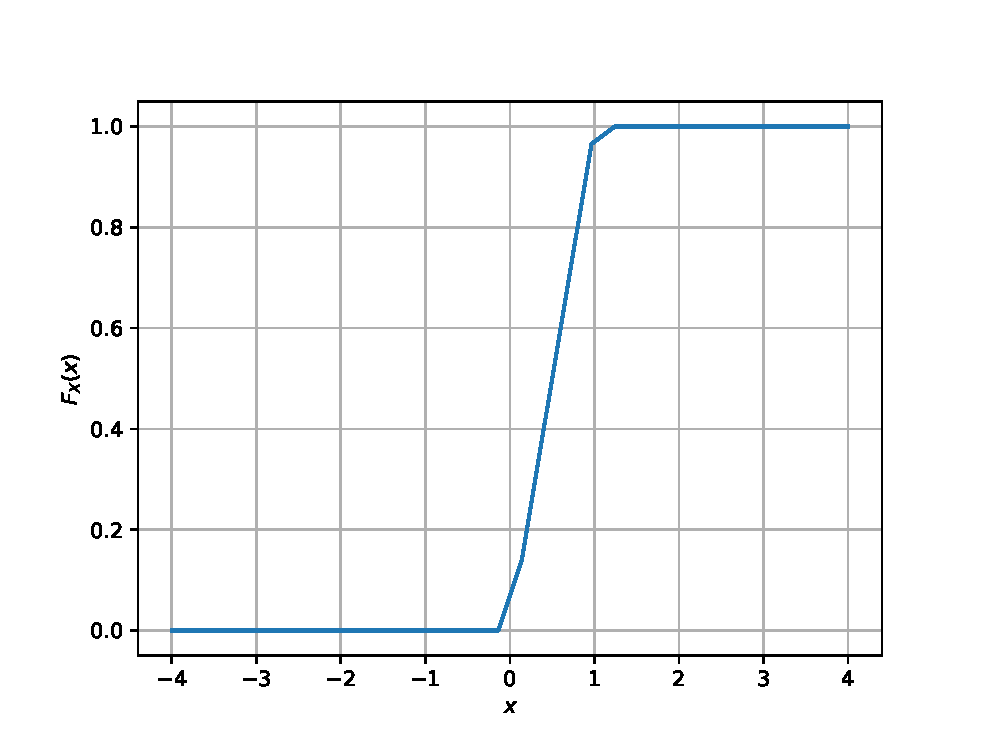
\includegraphics[width=\columnwidth]{./figs/uni_cdf}
\caption{The CDF of $U$}
\label{fig:uni_cdf}
\end{figure}

%
\item
Find a  theoretical expression for $F_{U}(x)$.

\item
The mean of $U$ is defined as
%
\begin{equation}
E\sbrak{U} = \frac{1}{N}\sum_{i=1}^{N}U_i
\end{equation}
%
and its variance as
%
\begin{equation}
\text{var}\sbrak{U} = E\sbrak{U- E\sbrak{U}}^2 
\end{equation}

Write a C program to  find the mean and variance of $U$. 
\item Verify your result theoretically given that
%
\begin{equation}
E\sbrak{U^k} = \int_{-\infty}^{\infty}x^kdF_{U}(x)
\end{equation}
\end{enumerate}
\section{Central Limit Theorem}
%
\begin{enumerate}[label=\thesection.\arabic*
,ref=\thesection.\theenumi]

%
\item
Generate $10^6$ samples of the random variable
%
\begin{equation}
X = \sum_{i=1}^{12}U_i -6
\end{equation}
%
using a C program, where $U_i, i = 1,2,\dots, 12$ are  a set of independent uniform random variables between 0 and 1
and save in a file called gau.dat

%
\item
Load gau.dat in python and plot the empirical CDF of $X$ using the samples in gau.dat. What properties does a CDF have?
\\
\solution The CDF of $X$ is plotted in Fig. \ref{fig:gauss_cdf}
\begin{figure}
\centering
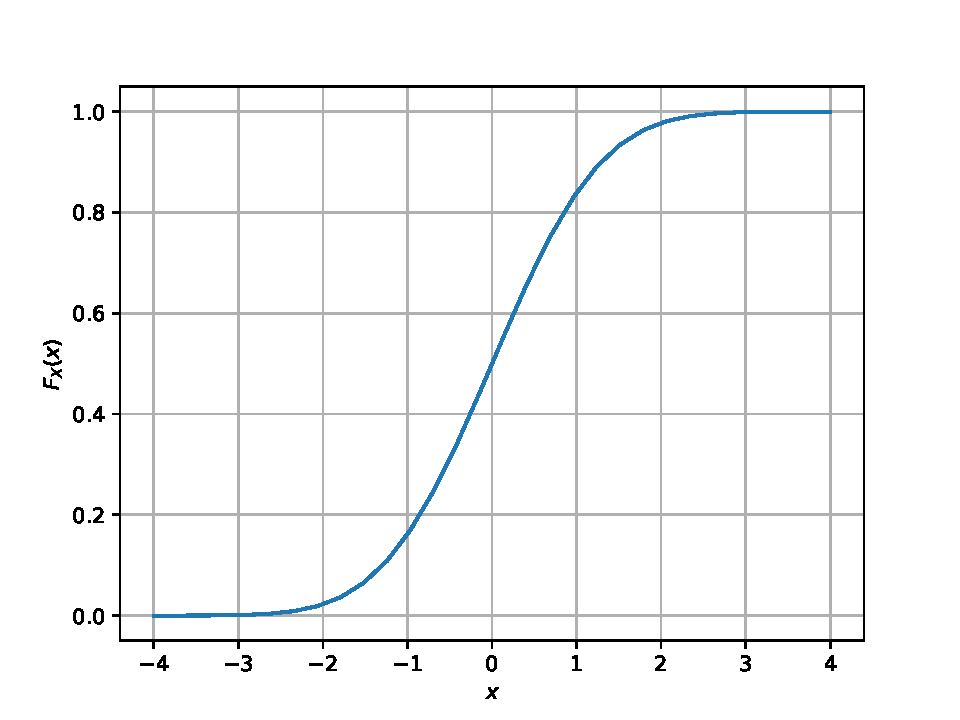
\includegraphics[width=\columnwidth]{./figs/gauss_cdf}
\caption{The CDF of $X$}
\label{fig:gauss_cdf}
\end{figure}
\item
Load gau.dat in python and plot the empirical PDF of $X$ using the samples in gau.dat. The PDF of $X$ is defined as
\begin{align}
p_{X}(x) = \frac{d}{dx}F_{X}(x)
\end{align}
What properties does the PDF have?
\\
\solution The PDF of $X$ is plotted in Fig. \ref{fig:gauss_pdf} using the code below
\begin{lstlisting}
codes/pdf_plot.py
\end{lstlisting}

\begin{figure}
\centering
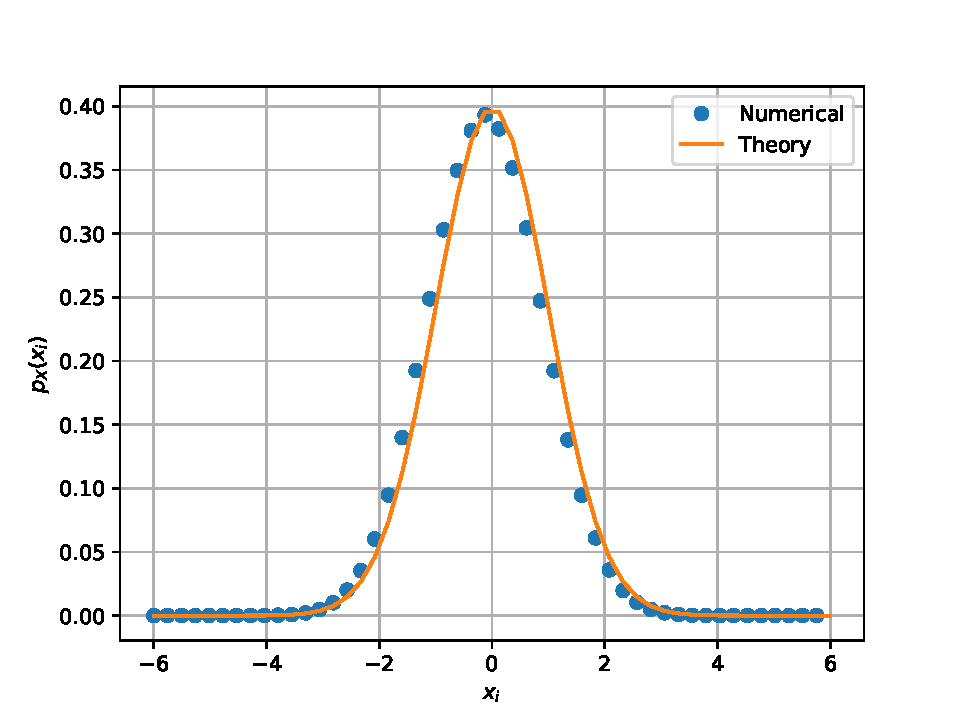
\includegraphics[width=\columnwidth]{./figs/gauss_pdf}
\caption{The PDF of $X$}
\label{fig:gauss_pdf}
\end{figure}

\item Find the mean and variance of $X$ by writing a C program.
\item Given that 
\begin{align}
p_{X}(x) = \frac{1}{\sqrt{2\pi}}\exp\brak{-\frac{x^2}{2}}, -\infty < x < \infty,
\end{align}
repeat the above exercise theoretically.
%
\end{enumerate}
\section{From Uniform to Other}
\begin{enumerate}[label=\thesection.\arabic*
,ref=\thesection.\theenumi]
%
\item
Generate samples of 
%
\begin{equation}
V = -2\ln\brak{1-U}
\end{equation}
%
and plot its CDF.  
\item Find a theoretical expression for $F_V(x)$.

%
%\item
%Generate the Rayleigh distribution from Uniform. Verify your result through graphical plots.
\end{enumerate}

\section{Triangular Distribution}
\begin{enumerate}[label=\thesection.\arabic*
,ref=\thesection.\theenumi]
%
\item Generate 
	\begin{align}
		T = U_1+U_2
	\end{align}
\item Find the CDF of $T$.
\item Find the PDF of $T$.
\item Find the theoretical expressions for the PDF and CDF of $T$.
\item Verify your results through a plot. 
\end{enumerate}
\section{Maximum Likelihood}
\begin{enumerate}[label=\thesection.\arabic*
,ref=\thesection.\theenumi]
\item Generate equiprobable $X \in \cbrak{1,-1}$.
\item Generate 
\begin{equation}
Y = AX+N,
\end{equation}
		where $A = 5$ dB,  and $N \sim \gauss{0}{1}$.
	\item Plot $Y$ using a scatter plot.
	\item Guess how to estimate $X$ from $Y$.
\item
\label{ml-ch4_sim}
Find 
\begin{equation}
	P_{e|0} = \pr{\hat{X} = -1|X=1}
\end{equation}
and 
\begin{equation}
	P_{e|1} = \pr{\hat{X} = 1|X=-1}
\end{equation}
%
\item Find $P_e$ assuming that $X$ has equiprobable symbols.

%
\item
Verify by plotting  the theoretical $P_e$ with respect to $A$ from 0 to 10 dB.  
%
\item Now, consider a threshold $\delta$  while estimating $X$ from $Y$. Find the value of $\delta$ that maximizes the theoretical $P_e$.
\item Repeat the above exercise when 
	\begin{align}
		p_{X}(0) = p
	\end{align}
\item Repeat the above exercise using the MAP criterion.

		\end{enumerate}
		\fi
\section{Gaussian to Other}
\begin{enumerate}[label=\thesection.\arabic*
,ref=\thesection.\theenumi]
\item
Let $X_1 \sim  \gauss{0}{1}$ and $X_2 \sim  \gauss{0}{1}$. Plot the CDF and PDF of
%
\begin{equation}
V = X_1^2 + X_2^2
\end{equation}
%

%
%
\item
If
%
\begin{equation}
F_{V}(x) = 
\begin{cases}
1 - e^{-\alpha x} & x \geq 0 \\
0 & x < 0,
\end{cases}
\end{equation}
%
find $\alpha$.

%
\item
\label{ch3_raleigh_sim}
Plot the CDF and PDf of
%
\begin{equation}
A = \sqrt{V}
\end{equation}
%


\end{enumerate}

\section{Conditional Probability}
\begin{enumerate}[label=\thesection.\arabic*
,ref=\thesection.\theenumi]
\item
\label{ch4_sim}
Plot 
\begin{equation}
P_e = \pr{\hat{X} = -1|X=1}
\end{equation}
%
for 
\begin{equation}
Y = AX+N,
\end{equation}
where $A$ is Raleigh with $E\sbrak{A^2} = \gamma, N \sim \gauss{0}{1}, X \in \brak{-1,1}$ for $0 \le \gamma \le 10$ dB.

%
\item
Assuming that $N$ is a constant, find an expression for $P_e$.  Call this $P_e(N)$

%
\item
%
\label{ch4_anal}
For a function $g$,
\begin{equation}
E\sbrak{g(X)} = \int_{-\infty}^{\infty}g(x)p_{X}(x)\, dx
\end{equation}
%
Find $P_e = E\sbrak{P_e(N)}$.

%
\item
Plot $P_e$ in problems \ref{ch4_sim} and \ref{ch4_anal} on the same graph w.r.t $\gamma$.  Comment.

		\end{enumerate}
		\iffalse
\section{Two Dimensions}
Let 
\begin{equation}
\mbf{y} = A\mbf{x} + \mbf{n},
\end{equation}
where 
\begin{align}
x &\in \brak{\mbf{s}_0,\mbf{s}_1}, 
\mbf{s}_0 = 
\begin{pmatrix}
1 
\\
0
\end{pmatrix},
\mbf{s}_1 = 
\begin{pmatrix}
0 
\\
1
\end{pmatrix}
\\
\mbf{n} &= 
\begin{pmatrix}
n_1
\\
n_2
\end{pmatrix},
n_1,n_2 \sim \gauss{0}{1}.
\end{align}
%
\begin{enumerate}[label=\thesection.\arabic*
,ref=\thesection.\theenumi]

%%
\item
\label{ch5_fsk}
Plot 
%
\begin{equation}
\mbf{y}|\mbf{s}_0 \text{ and } \mbf{y}|\mbf{s}_1
\end{equation}
%
on the same graph using a scatter plot.

%
\item
For the above problem, find a decision rule for detecting the symbols $\mbf{s}_0 $ and $\mbf{s}_1$.

%
\item
Plot 
\begin{equation} 
P_e = \pr{\hat{\mbf{x}} = \mbf{s}_1|\mbf{x} = \mbf{s}_0}
\end{equation}
with respect to the SNR from 0 to 10 dB.

%
\item
Obtain an expression for $P_e$. Verify this by comparing the theory and simulation plots on the same graph.

%
		\end{enumerate}
\end{document}
\fi

\chapter{Bivariate Random Variables: FSK}
\iffalse
\let\negmedspace\undefined
\let\negthickspace\undefined
\documentclass[journal,12pt,twocolumn]{IEEEtran}
%\documentclass[conference]{IEEEtran}
%\IEEEoverridecommandlockouts
% The preceding line is only needed to identify funding in the first footnote. If that is unneeded, please comment it out.
\usepackage{cite}
\usepackage{amssymb,amsfonts,amsthm,amsmath}
\usepackage{algorithmic}
\usepackage{graphicx}
\usepackage{textcomp}
\usepackage{xcolor}
\usepackage{txfonts}
\usepackage{listings}
\usepackage{enumitem}
\usepackage{mathtools}
\usepackage{gensymb}

%%
%\usepackage{setspace}
%%\doublespacing
%\singlespacing
%
%%\usepackage{graphicx}
%%\usepackage{amssymb}
%%\usepackage{relsize}
%\usepackage[cmex10]{amsmath}
%%\interdisplaylinepenalty=2500
%%\savesymbol{iint}
%%\usepackage{txfonts}
%%\restoresymbol{TXF}{iint}
%%\usepackage{wasysym}
%\usepackage{amsthm}
%\usepackage{mathrsfs}
%\usepackage{txfonts}
%%\usepackage{stfloats}
%%\usepackage{cite}
%%\usepackage{cases}
%%\usepackage{subfig}
%%\usepackage{xtab}
%%\usepackage{multirow}
%%\usepackage{algorithm}
%%\usepackage{algpseudocode}
%%\usepackage{tikz}
%%\usepackage{circuitikz}
%%\usepackage{verbatim}
\usepackage{hyperref}
%%\usepackage{stmaryrd}
%%\usepackage{tkz-euclide} % loads  TikZ and tkz-base
%%\usetkzobj{all}
    \usepackage{color}                                            %%
    \usepackage{array}                                            %%
    \usepackage{longtable}                                        %%
    \usepackage{calc}                                             %%
    \usepackage{multirow}                                         %%
    \usepackage{hhline}                                           %%
    \usepackage{ifthen}                                           %%
%  %optionally (for landscape tables embedded in another document): %%
%    \usepackage{lscape}     
%%\usepackage{multicol}
%\usepackage{chngcntr}
%\usepackage{enumerate}

%\usepackage{wasysym}
%\newcounter{MYtempeqncnt}
\DeclareMathOperator*{\Res}{Res}
%\renewcommand{\baselinestretch}{2}
\renewcommand\thesection{\arabic{section}}
\renewcommand\thesubsection{\thesection.\arabic{subsection}}
\renewcommand\thesubsubsection{\thesubsection.\arabic{subsubsection}}

\renewcommand\thesectiondis{\arabic{section}}
\renewcommand\thesubsectiondis{\thesectiondis.\arabic{subsection}}
\renewcommand\thesubsubsectiondis{\thesubsectiondis.\arabic{subsubsection}}

% correct bad hyphenation here
\hyphenation{op-tical net-works semi-conduc-tor}
\def\inputGnumericTable{}                                 %%

\lstset{
language=tex,
frame=single, 
breaklines=true
}

\begin{document}
%


\newtheorem{theorem}{Theorem}[section]
\newtheorem{problem}{Problem}
\newtheorem{proposition}{Proposition}[section]
\newtheorem{lemma}{Lemma}[section]
\newtheorem{corollary}[theorem]{Corollary}
\newtheorem{example}{Example}[section]
\newtheorem{definition}[problem]{Definition}
%\newtheorem{thm}{Theorem}[section] 
%\newtheorem{defn}[thm]{Definition}
%\newtheorem{algorithm}{Algorithm}[section]
%\newtheorem{cor}{Corollary}
\newcommand{\BEQA}{\begin{eqnarray}}
\newcommand{\EEQA}{\end{eqnarray}}
\newcommand{\define}{\stackrel{\triangle}{=}}

\bibliographystyle{IEEEtran}
%\bibliographystyle{ieeetr}


\providecommand{\mbf}{\mathbf}
\providecommand{\pr}[1]{\ensuremath{\Pr\left(#1\right)}}
\providecommand{\re}[1]{\ensuremath{\text{Re}\left(#1\right)}}
\providecommand{\im}[1]{\ensuremath{\text{Im}\left(#1\right)}}
\providecommand{\qfunc}[1]{\ensuremath{Q\left(#1\right)}}
\providecommand{\sbrak}[1]{\ensuremath{{}\left[#1\right]}}
\providecommand{\lsbrak}[1]{\ensuremath{{}\left[#1\right.}}
\providecommand{\rsbrak}[1]{\ensuremath{{}\left.#1\right]}}
\providecommand{\brak}[1]{\ensuremath{\left(#1\right)}}
\providecommand{\lbrak}[1]{\ensuremath{\left(#1\right.}}
\providecommand{\rbrak}[1]{\ensuremath{\left.#1\right)}}
\providecommand{\cbrak}[1]{\ensuremath{\left\{#1\right\}}}
\providecommand{\lcbrak}[1]{\ensuremath{\left\{#1\right.}}
\providecommand{\rcbrak}[1]{\ensuremath{\left.#1\right\}}}
\theoremstyle{remark}
\newtheorem{rem}{Remark}
\newcommand{\sgn}{\mathop{\mathrm{sgn}}}
\providecommand{\abs}[1]{\left\vert#1\right\vert}
\providecommand{\res}[1]{\Res\displaylimits_{#1}} 
\providecommand{\norm}[1]{\left\lVert#1\right\rVert}
%\providecommand{\norm}[1]{\lVert#1\rVert}
\providecommand{\mtx}[1]{\mathbf{#1}}
\providecommand{\mean}[1]{E\left[ #1 \right]}
\providecommand{\fourier}{\overset{\mathcal{F}}{ \rightleftharpoons}}
%\providecommand{\hilbert}{\overset{\mathcal{H}}{ \rightleftharpoons}}
\providecommand{\system}{\overset{\mathcal{H}}{ \longleftrightarrow}}
	%\newcommand{\solution}[2]{\textbf{Solution:}{#1}}
\newcommand{\solution}{\noindent \textbf{Solution: }}
\providecommand{\dec}[2]{\ensuremath{\overset{#1}{\underset{#2}{\gtrless}}}}
\newcommand{\myvec}[1]{\ensuremath{\begin{pmatrix}#1\end{pmatrix}}}
\newcommand{\mydet}[1]{\ensuremath{\begin{vmatrix}#1\end{vmatrix}}}
	\newcommand*{\permcomb}[4][0mu]{{{}^{#3}\mkern#1#2_{#4}}}
\newcommand*{\perm}[1][-3mu]{\permcomb[#1]{P}}
\newcommand*{\comb}[1][-1mu]{\permcomb[#1]{C}}
\providecommand{\gauss}[2]{\mathcal{N}\ensuremath{\left(#1,#2\right)}}
%%
%	%\newcommand{\solution}[2]{\textbf{Solution:}{#1}}
%\newcommand{\solution}{\noindent \textbf{Solution: }}
\newcommand{\cosec}{\,\text{cosec}\,}
\newcommand{\sinc}{\,\text{sinc}\,}
\newcommand{\rect}{\,\text{rect}\,}

%\numberwithin{equation}{section}
\numberwithin{equation}{subsection}
%\numberwithin{problem}{section}
%\numberwithin{definition}{section}
\makeatletter
\@addtoreset{figure}{problem}
\makeatother

\let\StandardTheFigure\thefigure
\let\vec\mathbf
\let\j\jmath
%\renewcommand{\thefigure}{\theproblem.\arabic{figure}}
\renewcommand{\thefigure}{\theproblem}
%\setlist[enumerate,1]{before=\renewcommand\theequation{\theenumi.\arabic{equation}}
%\counterwithin{equation}{enumi}


%\renewcommand{\theequation}{\arabic{subsection}.\arabic{equation}}

\def\putbox#1#2#3{\makebox[0in][l]{\makebox[#1][l]{}\raisebox{\baselineskip}[0in][0in]{\raisebox{#2}[0in][0in]{#3}}}}
     \def\rightbox#1{\makebox[0in][r]{#1}}
     \def\centbox#1{\makebox[0in]{#1}}
     \def\topbox#1{\raisebox{-\baselineskip}[0in][0in]{#1}}
     \def\midbox#1{\raisebox{-0.5\baselineskip}[0in][0in]{#1}}

\vspace{3cm}

\title{
%	\logo{
	Probability
%	}
}
%\title{
%	\logo{Matrix Analysis through Octave}{\begin{center}\includegraphics[scale=.24]{tlc}\end{center}}{}{HAMDSP}
%}


% paper title
% can use linebreaks \\ within to get better formatting as desired
%\title{Matrix Analysis through Octave}
%
%
% author names and IEEE memberships
% note positions of commas and nonbreaking spaces ( ~ ) LaTeX will not break
% a structure at a ~ so this keeps an author's name from being broken across
% two lines.
% use \thanks{} to gain access to the first footnote area
% a separate \thanks must be used for each paragraph as LaTeX2e's \thanks
% was not built to handle multiple paragraphs
%

\author{
	G. V. V. Sharma
	%<-this % stops a space
%\thanks{}}
}
% note the % following the last \IEEEmembership and also \thanks - 
% these prevent an unwanted space from occurring between the last author name
% and the end of the author line. i.e., if you had this:
% 
% \author{....lastname \thanks{...} \thanks{...} }
%                     ^------------^------------^----Do not want these spaces!
%
% a space would be appended to the last name and could cause every name on that
% line to be shifted left slightly. This is one of those "LaTeX things". For
% instance, "\textbf{A} \textbf{B}" will typeset as "A B" not "AB". To get
% "AB" then you have to do: "\textbf{A}\textbf{B}"
% \thanks is no different in this regard, so shield the last } of each \thanks
% that ends a line with a % and do not let a space in before the next \thanks.
% Spaces after \IEEEmembership other than the last one are OK (and needed) as
% you are supposed to have spaces between the names. For what it is worth,
% this is a minor point as most people would not even notice if the said evil
% space somehow managed to creep in.



% The paper headers
%\markboth{Journal of \LaTeX\ Class Files,~Vol.~6, No.~1, January~2007}%
%{Shell \MakeLowercase{\textit{et al.}}: Bare Demo of IEEEtran.cls for Journals}
% The only time the second header will appear is for the odd numbered pages
% after the title page when using the twoside option.
% 
% *** Note that you probably will NOT want to include the author's ***
% *** name in the headers of peer review papers.                   ***
% You can use \ifCLASSOPTIONpeerreview for conditional compilation here if
% you desire.




% If you want to put a publisher's ID mark on the page you can do it like
% this:
%\IEEEpubid{0000--0000/00\$00.00~\copyright~2007 IEEE}
% Remember, if you use this you must call \IEEEpubidadjcol in the second
% column for its text to clear the IEEEpubid mark.



% make the title area
\maketitle

\newpage

\tableofcontents

\bigskip

\renewcommand{\thefigure}{\theenumi}
\renewcommand{\thetable}{\theenumi}
%\renewcommand{\theequation}{\theenumi}

%\begin{abstract}
%%\boldmath
%In this letter, an algorithm for evaluating the exact analytical bit error rate  (BER)  for the piecewise linear (PL) combiner for  multiple relays is presented. Previous results were available only for upto three relays. The algorithm is unique in the sense that  the actual mathematical expressions, that are prohibitively large, need not be explicitly obtained. The diversity gain due to multiple relays is shown through plots of the analytical BER, well supported by simulations. 
%
%\end{abstract}
% IEEEtran.cls defaults to using nonbold math in the Abstract.
% This preserves the distinction between vectors and scalars. However,
% if the journal you are submitting to favors bold math in the abstract,
% then you can use LaTeX's standard command \boldmath at the very start
% of the abstract to achieve this. Many IEEE journals frown on math
% in the abstract anyway.

% Note that keywords are not normally used for peerreview papers.
%\begin{IEEEkeywords}
%Cooperative diversity, decode and forward, piecewise linear
%\end{IEEEkeywords}



% For peer review papers, you can put extra information on the cover
% page as needed:
% \ifCLASSOPTIONpeerreview
% \begin{center} \bfseries EDICS Category: 3-BBND \end{center}
% \fi
%
% For peerreview papers, this IEEEtran command inserts a page break and
% creates the second title. It will be ignored for other modes.
%\IEEEpeerreviewmaketitle

%\begin{abstract}
%\end{abstract}

%\iffalse





%% Copyright (C) 2020 Saurabh Joshi
%%% 
%\let\negmedspace\undefined
%\let\negthickspace\undefined
%
%\documentclass[journal,12pt,onecolumn]{IEEEtran}
%%\documentclass[journal,12pt,twocolumn]{IEEEtran}
%%
%\usepackage{setspace}
%\usepackage{gensymb}
%%\doublespacing
%\singlespacing
%
%%\usepackage{graphicx}
%%\usepackage{amssymb}
%%\usepackage{relsize}
%\usepackage[cmex10]{amsmath}
%%\usepackage{amsthm}
%%\interdisplaylinepenalty=2500
%%\savesymbol{iint}
%%\usepackage{txfonts}
%%\restoresymbol{TXF}{iint}
%%\usepackage{wasysym}
%\usepackage{amsthm}
%\usepackage{mathrsfs}
%\usepackage{txfonts}
%\usepackage{stfloats}
%\usepackage{cite}
%\usepackage{cases}
%\usepackage{subfig}
%%\usepackage{xtab}
%\usepackage{longtable}
%\usepackage{multirow}
%%\usepackage{algorithm}
%%\usepackage{algpseudocode}
%\usepackage{enumitem}
%\usepackage{mathtools}
%\usepackage{tikz}
%\usepackage{circuitikz}
%\usepackage{verbatim}
%\usepackage{hyperref}
%%\usepackage{stmaryrd}
%\usepackage{tkz-euclide} % loads  TikZ and tkz-base
%%\usetkzobj{all}
%\usepackage{listings}
%    \usepackage{color}                                            %%
%    \usepackage{array}                                            %%
%    \usepackage{longtable}                                        %%
%    \usepackage{calc}                                             %%
%    \usepackage{multirow}                                         %%
%    \usepackage{hhline}                                           %%
%    \usepackage{ifthen}                                           %%
%  %optionally (for landscape tables embedded in another document): %%
%    \usepackage{lscape}     
%\usepackage{multicol}
%\usepackage{chngcntr}
%\usepackage{iftex}
%%\usepackage[latin9]{inputenc}
%\usepackage{geometry}
%\usepackage{bm}
%%\geometry{verbose,tmargin=2cm,bmargin=3cm,lmargin=1.8cm,rmargin=1.5cm,headheight=2cm,headsep=2cm,footskip=3cm}
%\usepackage{array}
%\newcolumntype{L}[1]{>{\raggedright\let\newline\\\arraybackslash\hspace{0pt}}m{#1}}
%\newcolumntype{C}[1]{>{\centering\let\newline\\\arraybackslash\hspace{0pt}}m{#1}}
%\newcolumntype{R}[1]{>{\raggedleft\let\newline\\\arraybackslash\hspace{0pt}}m{#1}}
%
%%\usepackage{graphicx}
%%\usepackage{setspace}
%%\usepackage{parskip}
%
%\def \hsp {\hspace{3mm}}
%
%\makeatletter
%
%\providecommand{\tabularnewline}{\\}
%
%
%
%\makeatother
%\ifxetex
%\usepackage[T1]{fontenc}
%\usepackage{fontspec}
%%\setmainfont[ Path = fonts/]{Sanskrit_2003.ttf}
%\newfontfamily\nakulafont[Script=Devanagari,AutoFakeBold=2,Path = fonts/]{Nakula}
%%\newfontfamily\liberationfont{Liberation Sans Narrow}
%%\newfontfamily\liberationsansfont{Liberation Sans}
%\fi
%\usepackage{tikz}
%\usepackage{xcolor}
%%\usepackage{enumerate}
%
%%\usepackage{wasysym}
%%\newcounter{MYtempeqncnt}
%\DeclareMathOperator*{\Res}{Res}
%%\renewcommand{\baselinestretch}{2}
%\renewcommand\thesection{\arabic{section}}
%\renewcommand\thesubsection{\thesection.\arabic{subsection}}
%\renewcommand\thesubsubsection{\thesubsection.\arabic{subsubsection}}
%
%\renewcommand\thesectiondis{\arabic{section}}
%\renewcommand\thesubsectiondis{\thesectiondis.\arabic{subsection}}
%\renewcommand\thesubsubsectiondis{\thesubsectiondis.\arabic{subsubsection}}
%
%% correct bad hyphenation here
%\hyphenation{op-tical net-works semi-conduc-tor}
%\def\inputGnumericTable{}                                 %%
%
%\lstset{
%language=tex,
%frame=single, 
%breaklines=true
%}
%
%%\begin{document}
%%
%
%
%\newtheorem{theorem}{Theorem}[section]
%\newtheorem{problem}{Problem}
%\newtheorem{proposition}{Proposition}[section]
%\newtheorem{lemma}{Lemma}[section]
%\newtheorem{corollary}[theorem]{Corollary}
%\newtheorem{example}{Example}[section]
%\newtheorem{definition}[problem]{Definition}
%%\newtheorem{thm}{Theorem}[section] 
%%\newtheorem{defn}[thm]{Definition}
%%\newtheorem{algorithm}{Algorithm}[section]
%%\newtheorem{cor}{Corollary}
%\newcommand{\BEQA}{\begin{eqnarray}}
%\newcommand{\EEQA}{\end{eqnarray}}
%\newcommand{\define}{\stackrel{\triangle}{=}}
%
%\bibliographystyle{IEEEtran}
%%\bibliographystyle{ieeetr}
%
%
%\providecommand{\mbf}{\mathbf}
%\providecommand{\pr}[1]{\ensuremath{\Pr\left(#1\right)}}
%\providecommand{\qfunc}[1]{\ensuremath{Q\left(#1\right)}}
%\providecommand{\sbrak}[1]{\ensuremath{{}\left[#1\right]}}
%\providecommand{\lsbrak}[1]{\ensuremath{{}\left[#1\right.}}
%\providecommand{\rsbrak}[1]{\ensuremath{{}\left.#1\right]}}
%\providecommand{\brak}[1]{\ensuremath{\left(#1\right)}}
%\providecommand{\lbrak}[1]{\ensuremath{\left(#1\right.}}
%\providecommand{\rbrak}[1]{\ensuremath{\left.#1\right)}}
%\providecommand{\cbrak}[1]{\ensuremath{\left\{#1\right\}}}
%\providecommand{\lcbrak}[1]{\ensuremath{\left\{#1\right.}}
%\providecommand{\rcbrak}[1]{\ensuremath{\left.#1\right\}}}
%\theoremstyle{remark}
%\newtheorem{rem}{Remark}
%\newcommand{\sgn}{\mathop{\mathrm{sgn}}}
%\providecommand{\abs}[1]{\left\vert#1\right\vert}
%\providecommand{\res}[1]{\Res\displaylimits_{#1}} 
%\providecommand{\norm}[1]{\left\lVert#1\right\rVert}
%%\providecommand{\norm}[1]{\lVert#1\rVert}
%\providecommand{\mtx}[1]{\mathbf{#1}}
%\providecommand{\mean}[1]{E\left[ #1 \right]}
%%\numberwithin{equation}{section}
%\numberwithin{equation}{section}
%%\numberwithin{problem}{section}
%%\numberwithin{definition}{section}
%\makeatletter
%\@addtoreset{figure}{problem}
%\makeatother
%
%\let\StandardTheFigure\thefigure
%\let\vec\mathbf
%%\renewcommand{\thefigure}{\theproblem.\arabic{figure}}
%\renewcommand{\thefigure}{\theproblem}
%%\setlist[enumerate,1]{before=\renewcommand\theequation{\theenumi.\arabic{equation}}
%%\counterwithin{equation}{enumi}
%
%
%%\renewcommand{\theequation}{\arabic{subsection}.\arabic{equation}}
%
%\vspace{3cm}
%
%
%%\usepackage{babel}
%\begin{document}
%
%\begin{tabular}{L{6cm} C{5cm} R{5cm} }
%
%	\definecolor{circleorange}{rgb}{1,0.17,0.08}
%\definecolor{darkorange}{rgb}{1,0.27,0.1}
%\definecolor{orange2}{rgb}{1,0.5,0.15}
%\definecolor{orange3}{rgb}{1,0.65,0.25}
%\definecolor{yellow1}{rgb}{0.95,0.77,0.2}
%%\begin{tikzpicture}[scale=0.2,every node/.style={transform shape}]
%\begin{tikzpicture}[scale=0.1,every node/.style={transform shape}]
%\draw [fill=circleorange,circleorange] (5,10) circle (1.15); 
%\fill [darkorange] (5.06,8) -- (5.06,2) -- (7.3,1.2) -- (7.3,8.8) -- (5.06,8);
%\fill [darkorange] (4.94,8) -- (4.94,2) -- (2.7,1.2) -- (2.7,8.8) -- (4.94,8);
%\fill [orange2]    (7.4,8.4) -- (7.4,1.6) -- (8.2,1.2) -- (8.2,8.8) -- (7.4,8.4);
%\fill [orange2]    (2.6,8.4) -- (2.6,1.6) -- (1.8,1.2) -- (1.8,8.8) -- (2.6,8.4);
%\fill [orange3]    (8.3,8.4) -- (8.3,1.6) -- (9.0,1.2) -- (9.0,8.8) -- (8.3,8.4);
%\fill [orange3]    (1.7,8.4) -- (1.7,1.6) -- (1.0,1.2) -- (1.0,8.8) -- (1.7,8.4);
%\fill [yellow1]    (9.1,8.4) -- (9.1,1.6) -- (9.7,1.2) -- (9.7,8.8) -- (9.1,8.4);
%\fill [yellow1]    (0.9,8.4) -- (0.9,1.6) -- (0.3,1.2) -- (0.3,8.8) -- (0.9,8.4);
%\ifxetex
%\node [scale=2.1] at (5,-0.1)  {   {\bf {\nakulafont  भारतीय प्रौद्योगिकी संस्थान हैदराबाद }} };
%\node [scale=1.8] at (5,-1.2) {   {\bf { Indian Institute of Technology Hyderabad}} };
%%\node [scale=1.8] at (5,-1.2) {   {\bf {\liberationsansfont Indian Institute of Technology Hyderabad}} };
%\fi
%\end{tikzpicture}
%% \includegraphics[scale=0.05]{logo_iith} \newline
%
%& Assignments 
%	&
%	AI1110
%\end{tabular}
%
%
%\vspace{-6mm}
%\begin{center}
%%\includegraphics[scale=0.95]{Yellow-Line}
%\begin{tikzpicture}
%\definecolor{yellow1}{rgb}{0.95,0.77,0.2}
%\draw[line width=0.75mm, yellow1] (0,0) -- (\textwidth,0);
%\end{tikzpicture}
%\par\end{center}
		\numberwithin{equation}{enumi}
\section{Uniform Random Numbers}
Let $U$ be a uniform random variable between 0 and 1.
\begin{enumerate}[label=\thesection.\arabic*
,ref=\thesection.\theenumi]
\item Generate $10^6$ samples of $U$ using a C program and save into a file called uni.dat .
\\
\solution Download the following files and execute the  C program.
\begin{lstlisting}
codes/exrand.c
codes/coeffs.h
\end{lstlisting}

%
\item
Load the uni.dat file into python and plot the empirical CDF of $U$ using the samples in uni.dat. The CDF is defined as
\begin{align}
F_{U}(x) = \pr{U \le x}
\end{align}
\\
\solution  The following code plots Fig. \ref{fig:uni_cdf}
\begin{lstlisting}
codes/cdf_plot.py
\end{lstlisting}
\begin{figure}
\centering
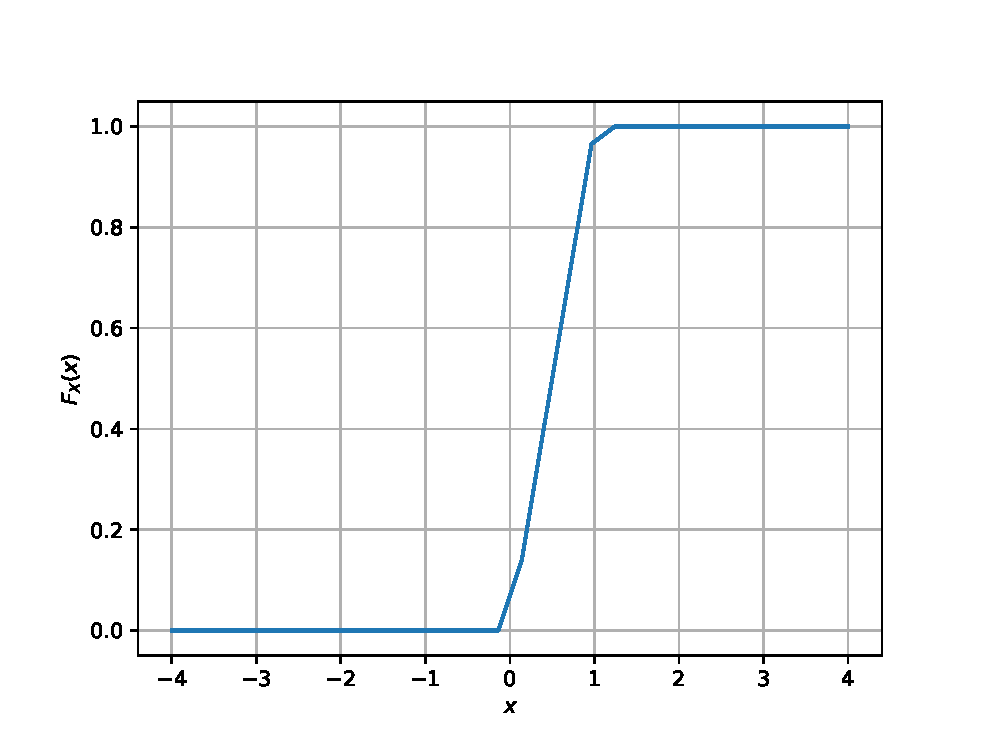
\includegraphics[width=\columnwidth]{./figs/uni_cdf}
\caption{The CDF of $U$}
\label{fig:uni_cdf}
\end{figure}

%
\item
Find a  theoretical expression for $F_{U}(x)$.

\item
The mean of $U$ is defined as
%
\begin{equation}
E\sbrak{U} = \frac{1}{N}\sum_{i=1}^{N}U_i
\end{equation}
%
and its variance as
%
\begin{equation}
\text{var}\sbrak{U} = E\sbrak{U- E\sbrak{U}}^2 
\end{equation}

Write a C program to  find the mean and variance of $U$. 
\item Verify your result theoretically given that
%
\begin{equation}
E\sbrak{U^k} = \int_{-\infty}^{\infty}x^kdF_{U}(x)
\end{equation}
\end{enumerate}
\section{Central Limit Theorem}
%
\begin{enumerate}[label=\thesection.\arabic*
,ref=\thesection.\theenumi]

%
\item
Generate $10^6$ samples of the random variable
%
\begin{equation}
X = \sum_{i=1}^{12}U_i -6
\end{equation}
%
using a C program, where $U_i, i = 1,2,\dots, 12$ are  a set of independent uniform random variables between 0 and 1
and save in a file called gau.dat

%
\item
Load gau.dat in python and plot the empirical CDF of $X$ using the samples in gau.dat. What properties does a CDF have?
\\
\solution The CDF of $X$ is plotted in Fig. \ref{fig:gauss_cdf}
\begin{figure}
\centering
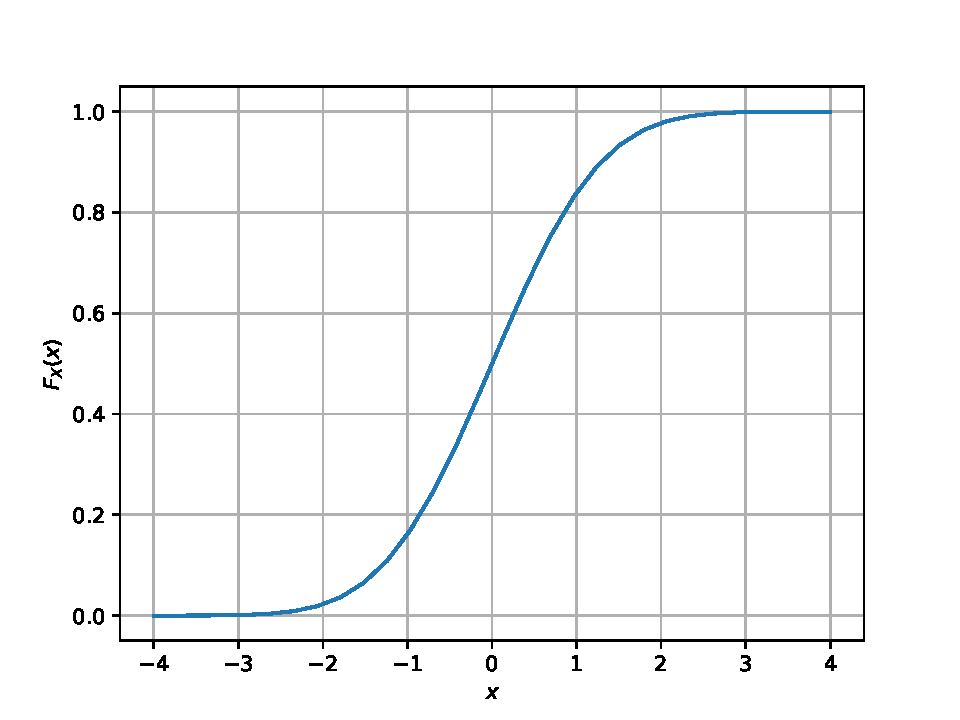
\includegraphics[width=\columnwidth]{./figs/gauss_cdf}
\caption{The CDF of $X$}
\label{fig:gauss_cdf}
\end{figure}
\item
Load gau.dat in python and plot the empirical PDF of $X$ using the samples in gau.dat. The PDF of $X$ is defined as
\begin{align}
p_{X}(x) = \frac{d}{dx}F_{X}(x)
\end{align}
What properties does the PDF have?
\\
\solution The PDF of $X$ is plotted in Fig. \ref{fig:gauss_pdf} using the code below
\begin{lstlisting}
codes/pdf_plot.py
\end{lstlisting}

\begin{figure}
\centering
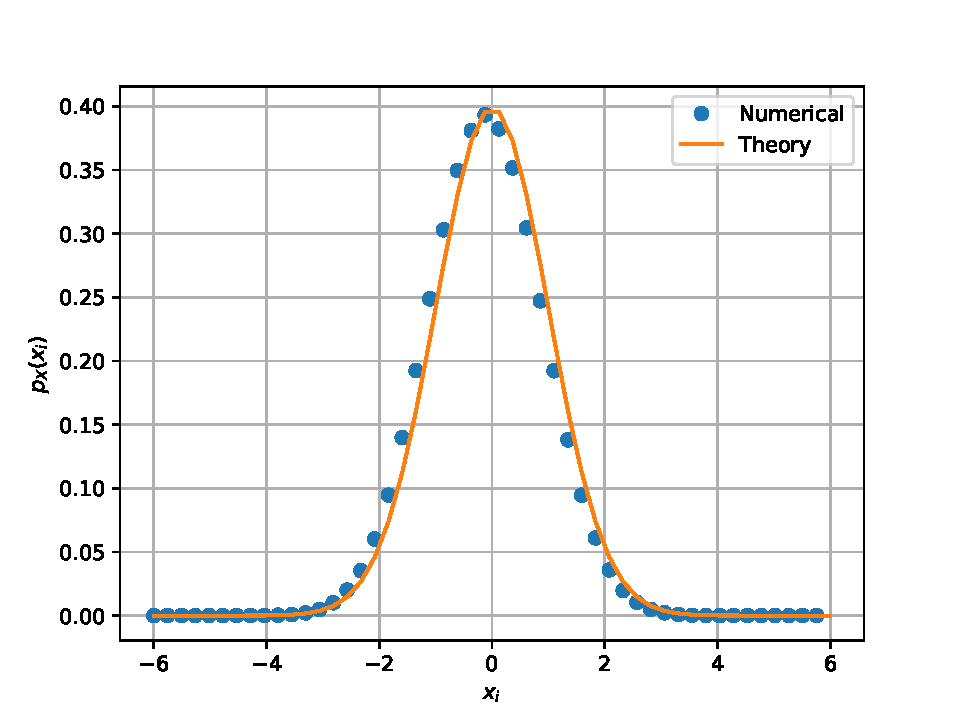
\includegraphics[width=\columnwidth]{./figs/gauss_pdf}
\caption{The PDF of $X$}
\label{fig:gauss_pdf}
\end{figure}

\item Find the mean and variance of $X$ by writing a C program.
\item Given that 
\begin{align}
p_{X}(x) = \frac{1}{\sqrt{2\pi}}\exp\brak{-\frac{x^2}{2}}, -\infty < x < \infty,
\end{align}
repeat the above exercise theoretically.
%
\end{enumerate}
\section{From Uniform to Other}
\begin{enumerate}[label=\thesection.\arabic*
,ref=\thesection.\theenumi]
%
\item
Generate samples of 
%
\begin{equation}
V = -2\ln\brak{1-U}
\end{equation}
%
and plot its CDF.  
\item Find a theoretical expression for $F_V(x)$.

%
%\item
%Generate the Rayleigh distribution from Uniform. Verify your result through graphical plots.
\end{enumerate}

\section{Triangular Distribution}
\begin{enumerate}[label=\thesection.\arabic*
,ref=\thesection.\theenumi]
%
\item Generate 
	\begin{align}
		T = U_1+U_2
	\end{align}
\item Find the CDF of $T$.
\item Find the PDF of $T$.
\item Find the theoretical expressions for the PDF and CDF of $T$.
\item Verify your results through a plot. 
\end{enumerate}
\section{Maximum Likelihood}
\begin{enumerate}[label=\thesection.\arabic*
,ref=\thesection.\theenumi]
\item Generate equiprobable $X \in \cbrak{1,-1}$.
\item Generate 
\begin{equation}
Y = AX+N,
\end{equation}
		where $A = 5$ dB,  and $N \sim \gauss{0}{1}$.
	\item Plot $Y$ using a scatter plot.
	\item Guess how to estimate $X$ from $Y$.
\item
\label{ml-ch4_sim}
Find 
\begin{equation}
	P_{e|0} = \pr{\hat{X} = -1|X=1}
\end{equation}
and 
\begin{equation}
	P_{e|1} = \pr{\hat{X} = 1|X=-1}
\end{equation}
%
\item Find $P_e$ assuming that $X$ has equiprobable symbols.

%
\item
Verify by plotting  the theoretical $P_e$ with respect to $A$ from 0 to 10 dB.  
%
\item Now, consider a threshold $\delta$  while estimating $X$ from $Y$. Find the value of $\delta$ that maximizes the theoretical $P_e$.
\item Repeat the above exercise when 
	\begin{align}
		p_{X}(0) = p
	\end{align}
\item Repeat the above exercise using the MAP criterion.

		\end{enumerate}
\section{Gaussian to Other}
\begin{enumerate}[label=\thesection.\arabic*
,ref=\thesection.\theenumi]
\item
Let $X_1 \sim  \gauss{0}{1}$ and $X_2 \sim  \gauss{0}{1}$. Plot the CDF and PDF of
%
\begin{equation}
V = X_1^2 + X_2^2
\end{equation}
%

%
%
\item
If
%
\begin{equation}
F_{V}(x) = 
\begin{cases}
1 - e^{-\alpha x} & x \geq 0 \\
0 & x < 0,
\end{cases}
\end{equation}
%
find $\alpha$.

%
\item
\label{ch3_raleigh_sim}
Plot the CDF and PDf of
%
\begin{equation}
A = \sqrt{V}
\end{equation}
%


\end{enumerate}

\section{Conditional Probability}
\begin{enumerate}[label=\thesection.\arabic*
,ref=\thesection.\theenumi]
\item
\label{ch4_sim}
Plot 
\begin{equation}
P_e = \pr{\hat{X} = -1|X=1}
\end{equation}
%
for 
\begin{equation}
Y = AX+N,
\end{equation}
where $A$ is Raleigh with $E\sbrak{A^2} = \gamma, N \sim \gauss{0}{1}, X \in \brak{-1,1}$ for $0 \le \gamma \le 10$ dB.

%
\item
Assuming that $N$ is a constant, find an expression for $P_e$.  Call this $P_e(N)$

%
\item
%
\label{ch4_anal}
For a function $g$,
\begin{equation}
E\sbrak{g(X)} = \int_{-\infty}^{\infty}g(x)p_{X}(x)\, dx
\end{equation}
%
Find $P_e = E\sbrak{P_e(N)}$.

%
\item
Plot $P_e$ in problems \ref{ch4_sim} and \ref{ch4_anal} on the same graph w.r.t $\gamma$.  Comment.

		\end{enumerate}
		\fi
\section{Two Dimensions}
Let 
\begin{equation}
\mbf{y} = A\mbf{x} + \mbf{n},
\end{equation}
where 
\begin{align}
x &\in \brak{\mbf{s}_0,\mbf{s}_1}, 
\mbf{s}_0 = 
\begin{pmatrix}
1 
\\
0
\end{pmatrix},
\mbf{s}_1 = 
\begin{pmatrix}
0 
\\
1
\end{pmatrix}
\\
\mbf{n} &= 
\begin{pmatrix}
n_1
\\
n_2
\end{pmatrix},
n_1,n_2 \sim \gauss{0}{1}.
\end{align}
%
\begin{enumerate}[label=\thesection.\arabic*
,ref=\thesection.\theenumi]

%%
\item
\label{ch5_fsk}
Plot 
%
\begin{equation}
\mbf{y}|\mbf{s}_0 \text{ and } \mbf{y}|\mbf{s}_1
\end{equation}
%
on the same graph using a scatter plot.

%
\item
For the above problem, find a decision rule for detecting the symbols $\mbf{s}_0 $ and $\mbf{s}_1$.

%
\item
Plot 
\begin{equation} 
P_e = \pr{\hat{\mbf{x}} = \mbf{s}_1|\mbf{x} = \mbf{s}_0}
\end{equation}
with respect to the SNR from 0 to 10 dB.

%
\item
Obtain an expression for $P_e$. Verify this by comparing the theory and simulation plots on the same graph.

%
		\end{enumerate}
		\iffalse
\end{document}
\fi

\chapter{Exercises}
\iffalse
\documentclass[journal,12pt,twocolumn]{IEEEtran}
%
\usepackage{setspace}
\usepackage{gensymb}
\usepackage{xcolor}
\usepackage{caption}
%\usepackage{subcaption}
%\doublespacing
\singlespacing
\usepackage{multicol}

\usepackage{iithtlc}
%\usepackage{graphicx}
%\usepackage{amssymb}
%\usepackage{relsize}
\usepackage[cmex10]{amsmath}
\usepackage{mathtools}
%\usepackage{amsthm}
%\interdisplaylinepenalty=2500
%\savesymbol{iint}
%\usepackage{txfonts}
%\restoresymbol{TXF}{iint}
%\usepackage{wasysym}
\usepackage{amsthm}
\usepackage{mathrsfs}
\usepackage{txfonts}
\usepackage{stfloats}
\usepackage{cite}
\usepackage{cases}
\usepackage{subfig}
%\usepackage{xtab}
\usepackage{longtable}
\usepackage{multirow}
%\usepackage{algorithm}
%\usepackage{algpseudocode}
\usepackage{enumitem}
\usepackage{mathtools}
%\usepackage{stmaryrd}

\usepackage{listings}
    \usepackage[latin1]{inputenc}                                 %%
    \usepackage{color}                                            %%
    \usepackage{array}                                            %%
    \usepackage{longtable}                                        %%
    \usepackage{calc}                                             %%
    \usepackage{multirow}                                         %%
    \usepackage{hhline}                                           %%
    \usepackage{ifthen}                                           %%
  %optionally (for landscape tables embedded in another document): %%
    \usepackage{lscape}     

%\usepackage{wasysym}
%\newcounter{MYtempeqncnt}
\DeclareMathOperator*{\Res}{Res}
%\renewcommand{\baselinestretch}{2}
\renewcommand\thesection{\arabic{section}}
\renewcommand\thesubsection{\thesection.\arabic{subsection}}
\renewcommand\thesubsubsection{\thesubsection.\arabic{subsubsection}}

\renewcommand\thesectiondis{\arabic{section}}
\renewcommand\thesubsectiondis{\thesectiondis.\arabic{subsection}}
\renewcommand\thesubsubsectiondis{\thesubsectiondis.\arabic{subsubsection}}

% correct bad hyphenation here
\hyphenation{op-tical net-works semi-conduc-tor}

\def\inputGnumericTable{}  

\lstset{
language=python,
frame=single, 
breaklines=true
}

\begin{document}
%

\theoremstyle{definition}

\newtheorem{theorem}{Theorem}[section]
\newtheorem{problem}{Problem}
\newtheorem{proposition}{Proposition}[section]
\newtheorem{lemma}{Lemma}[section]
\newtheorem{corollary}[theorem]{Corollary}
\newtheorem{example}{Example}[section]
\newtheorem{definition}{Definition}[section]
%\newtheorem{algorithm}{Algorithm}[section]
%\newtheorem{cor}{Corollary}
\newcommand{\BEQA}{\begin{eqnarray}}
\newcommand{\EEQA}{\end{eqnarray}}
\newcommand{\triangleq}{\stackrel{\triangle}{=}}

\bibliographystyle{IEEEtran}
%\bibliographystyle{ieeetr}



\providecommand{\pr}[1]{\ensuremath{\Pr\left(#1\right)}}
\providecommand{\qfunc}[1]{\ensuremath{Q\left(#1\right)}}
\providecommand{\sbrak}[1]{\ensuremath{{}\left[#1\right]}}
\providecommand{\lsbrak}[1]{\ensuremath{{}\left[#1\right.}}
\providecommand{\rsbrak}[1]{\ensuremath{{}\left.#1\right]}}
\providecommand{\brak}[1]{\ensuremath{\left(#1\right)}}
\providecommand{\lbrak}[1]{\ensuremath{\left(#1\right.}}
\providecommand{\rbrak}[1]{\ensuremath{\left.#1\right)}}
\providecommand{\cbrak}[1]{\ensuremath{\left\{#1\right\}}}
\providecommand{\lcbrak}[1]{\ensuremath{\left\{#1\right.}}
\providecommand{\rcbrak}[1]{\ensuremath{\left.#1\right\}}}
\theoremstyle{remark}
\newtheorem{rem}{Remark}
\newcommand{\sgn}{\mathop{\mathrm{sgn}}}
\providecommand{\abs}[1]{\left\vert#1\right\vert}
\providecommand{\res}[1]{\Res\displaylimits_{#1}} 
\providecommand{\norm}[1]{\lVert#1\rVert}
\providecommand{\mtx}[1]{\mathbf{#1}}
\providecommand{\mean}[1]{E\left[ #1 \right]}
\providecommand{\fourier}{\overset{\mathcal{F}}{ \rightleftharpoons}}
%\providecommand{\hilbert}{\overset{\mathcal{H}}{ \rightleftharpoons}}
\providecommand{\system}{\overset{\mathcal{H}}{ \longleftrightarrow}}
\providecommand{\gauss}[2]{\mathcal{N}\ensuremath{\left(#1,#2\right)}}
	%\newcommand{\solution}[2]{\textbf{Solution:}{#1}}
\newcommand{\solution}{\noindent \textbf{Solution: }}
\providecommand{\dec}[2]{\ensuremath{\overset{#1}{\underset{#2}{\gtrless}}}}
%\numberwithin{equation}{section}
%\numberwithin{problem}{section}

\def\putbox#1#2#3{\makebox[0in][l]{\makebox[#1][l]{}\raisebox{\baselineskip}[0in][0in]{\raisebox{#2}[0in][0in]{#3}}}}
     \def\rightbox#1{\makebox[0in][r]{#1}}
     \def\centbox#1{\makebox[0in]{#1}}
     \def\topbox#1{\raisebox{-\baselineskip}[0in][0in]{#1}}
     \def\midbox#1{\raisebox{-0.5\baselineskip}[0in][0in]{#1}}


% paper title
% can use linebreaks \\ within to get better formatting as desired
\title{
%\logo{
Digital Modulation Techniques
%}
}
%
%
% author names and IEEE memberships
% note positions of commas and nonbreaking spaces ( ~ ) LaTeX will not break
% a structure at a ~ so this keeps an author's name from being broken across
% two lines.
% use \thanks{} to gain access to the first footnote area
% a separate \thanks must be used for each paragraph as LaTeX2e's \thanks
% was not built to handle multiple paragraphs
%

%\author{Y Aditya, A Rathnakar and G V V Sharma$^{*}$% <-this % stops a space
\author{P.~N.~V.~S.~S.~K.~ HAVISH, S.~S.~Ashish and G V V Sharma %<-this  stops a space
\thanks{The authors are with the Department
of Electrical Engineering, IIT, Hyderabad
502285 India e-mail: \{ee16btech11023,ee16btech11043,jbala,gadepall\}@iith.ac.in. All material in the manuscript is released under GNU GPL.  Free to use for all.
}}



% make the title area
\maketitle

\tableofcontents

\bigskip

\begin{abstract}
%\boldmath
The manual frames the problems of receiver design and performance analysis in digital communication as applications of probability theory.

\end{abstract}
% IEEEtran.cls defaults to using nonbold math in the Abstract.
% This preserves the distinction between vectors and scalars. However,
% if the journal you are submitting to favors bold math in the abstract,
% then you can use LaTeX's standard command \boldmath at the very start
% of the abstract to achieve this. Many IEEE journals frown on math
% in the abstract anyway.

% Note that keywords are not normally used for peerreview papers.
%\begin{IEEEkeywords}
%Cooperative diversity, decode and forward, piecewise linear
%\end{IEEEkeywords}



% For peer review papers, you can put extra information on the cover
% page as needed:
% \ifCLASSOPTIONpeerreview
% \begin{center} \bfseries EDICS Category: 3-BBND \end{center}
% \fi
%
% For peerreview papers, this IEEEtran command inserts a page break and
% creates the second title. It will be ignored for other modes.
\IEEEpeerreviewmaketitle

\fi
\section{BPSK}
\begin{enumerate}
\item
The {\em signal constellation diagram} for BPSK is given by Fig. \ref{fig:bpsk_const}.  The symbols $s_0$ and $s_1$ are equiprobable.  $\sqrt{E_b}$ is the energy transmitted per bit. Assuming a zero mean additive white gaussian noise (AWGN) with variance $\frac{N_0}{2}$,
obtain the symbols that are received.

%
\begin{figure}[!h]
\centering
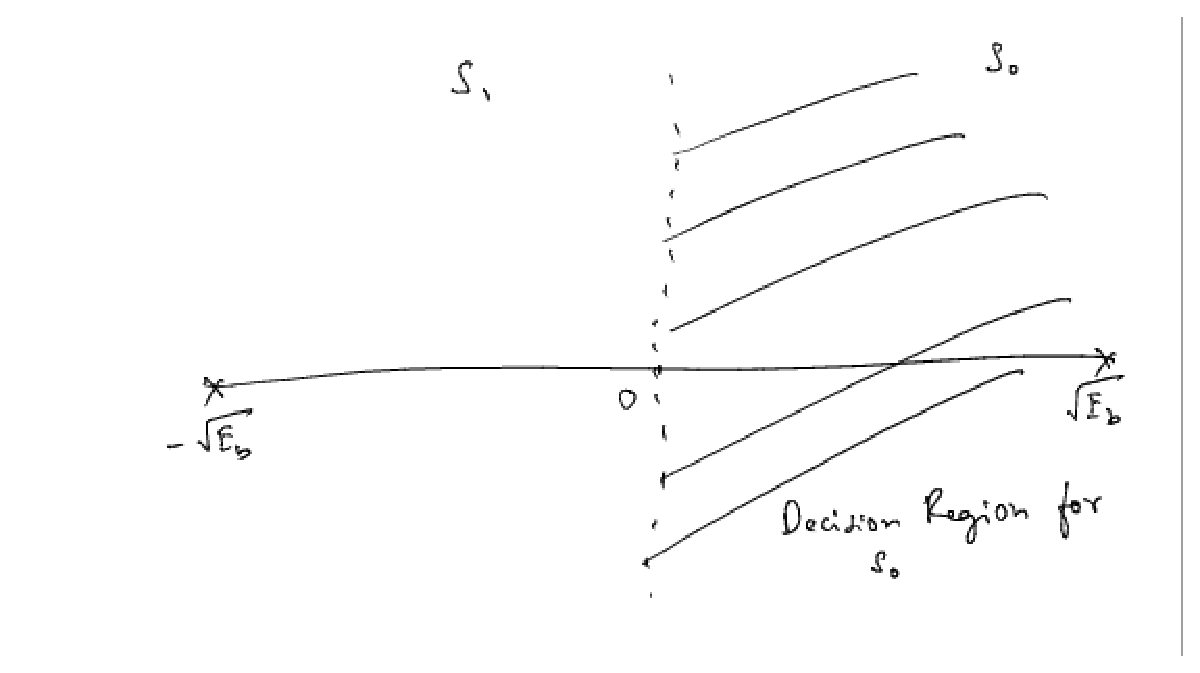
\includegraphics[width=\columnwidth]{./manual/figs/bpsk_const.eps}
\caption{}
\label{fig:bpsk_const}
\end{figure}
\solution The possible received symbols are
\begin{align}
y|s_0 &= \sqrt{E_b} + n
\\
y|s_1 &= -\sqrt{E_b} + n
\end{align}
%
where the AWGN $n \sim \gauss{0}{\frac{N_0}{2}}$.
%
\item
\label{prob:bpsk_decision}
From Fig. \ref{fig:bpsk_const} obtain a decision rule for BPSK

\solution The decision rule is
\begin{equation}
y \dec{s_0}{s_1} 0
\end{equation}
\item
Repeat the previous exercise using the MAP criterion.

\item
Using the decision rule in Problem \ref{prob:bpsk_decision}, obtain an expression for the probability of error for BPSK.

\solution
Since the symbols are equiprobable, it is sufficient if the error is calculated assuming that a 0 was sent.  This results in
\begin{align}
P_e &= \pr{y < 0|s_0} = \pr{\sqrt{E_b} + n < 0}
\\
&= \pr{ -n > \sqrt{E_b} } = \pr{ n > \sqrt{E_b} }
\label{eq:bpsk_proof_n0}
\end{align}
since $n$ has a symmetric pdf.
Let $w \sim \gauss{0}{1}$.  Then $n = \sqrt{\frac{N_0}{2}}w$. Substituting this in \eqref{eq:bpsk_proof_n0},
\begin{align}
P_e &=  \pr{ \sqrt{\frac{N_0}{2}}w > \sqrt{E_b} } = \pr{ w > \sqrt{\frac{2E_b}{N_0}} }
\\
&= \qfunc{\sqrt{\frac{2E_b}{N_0}}}
\end{align}
%
where $\qfunc{x} \triangleq \pr{w > x}, x \ge 0$.
\item
The PDF of $w \sim \gauss{0}{1}$ is given by
%
\begin{equation}
p_{w}(x) = \frac{1}{\sqrt{2\pi}}\exp\brak{-\frac{x^2}{2}}, -\infty < x < \infty
\end{equation}
and the complementary error function is defined as
\begin{equation}
\operatorname {erfc} (x)={\frac {2}{\sqrt {\pi }}}\int _{x}^{\infty }e^{-t^{2}}\,dt.
\end{equation}
%
Show that 
\begin{equation}
Q(x) = \frac{1}{2}\operatorname {erfc}\left({\frac  {x}{{\sqrt  {2}}}}\right)
\end{equation}

\item
Verify the bit error rate (BER) plots for BPSK through simulation and analysis for 0 to 10 dB.

\solution
The following code
%\lstinputlisting{./codes/bpsk_ber.py}
%\iffalse
\begin{lstlisting}
codes/bpsk_ber.py
\end{lstlisting}
%	\fi
yields Fig. \ref{fig:bpsk_ber}
\begin{figure}[!h]
\centering
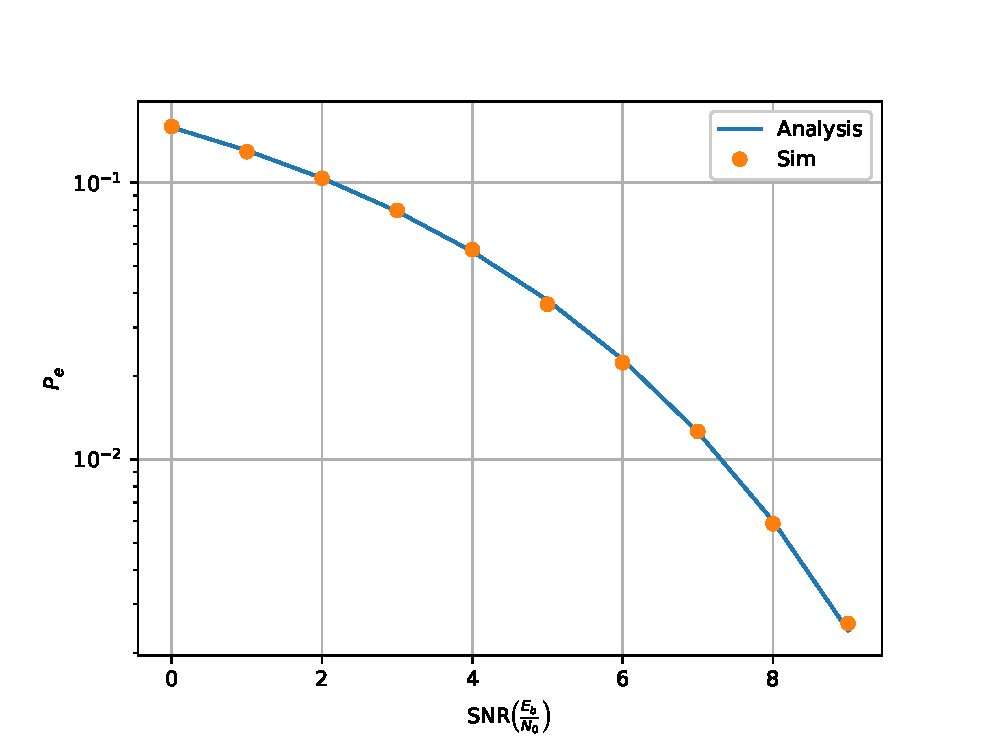
\includegraphics[width=\columnwidth]{./manual/figs/bpsk_ber.eps}
\caption{}
\label{fig:bpsk_ber}
\end{figure}

\item
Show that
\begin{equation}
Q(x) = \frac{1}{\pi}\int^{\frac{\pi}{2}}_{0}e^{-\frac{x^2}{2\sin^2 \theta}}\,d\theta
\end{equation}
\end{enumerate}
\section{Coherent BFSK}
\begin{enumerate}
\item
The signal constellation for binary frequency shift keying (BFSK) is given in Fig. \ref{fig:bfsk_const}.
Obtain the equations for the received symbols.

\begin{figure}[!h]
\centering
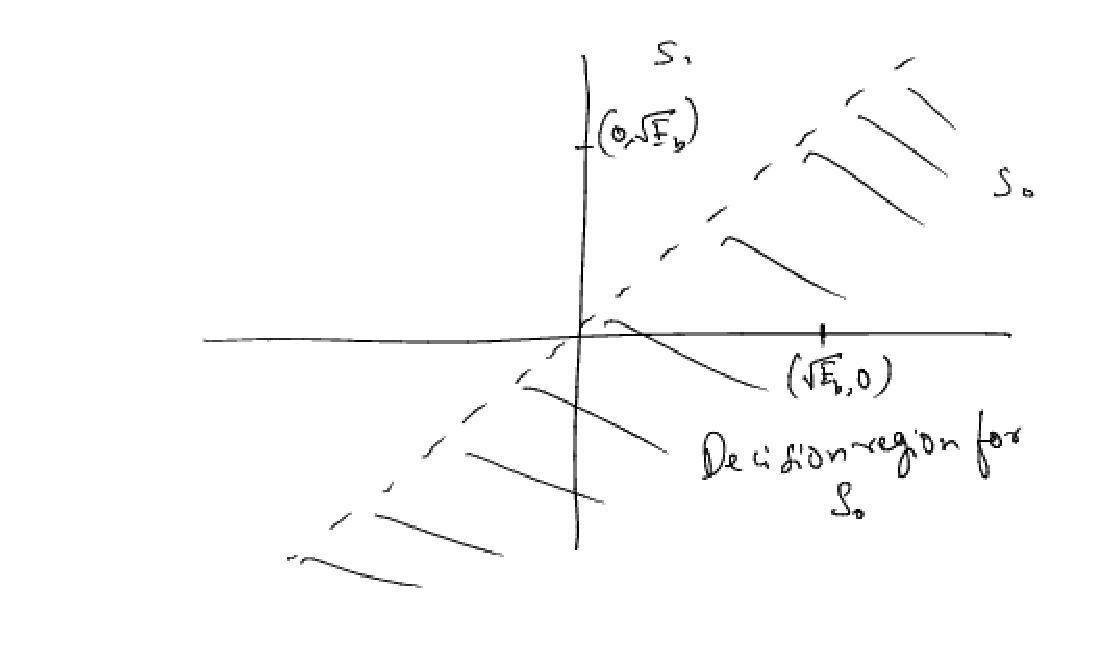
\includegraphics[width=\columnwidth]{./manual/figs/bfsk_const.eps}
\caption{}
\label{fig:bfsk_const}
\end{figure}
\solution
The received symbols are given by
\begin{align}
\mathbf{y}|s_0 = 
\myvec{
\sqrt{E_b} \\
0
}
+
\myvec{
 n_{1}\\
n_{2}
},
\end{align}
and 
\begin{align}
\mathbf{y}|s_1 = 
\myvec{
0\\
\sqrt{E_b} 
}
+
\myvec{
n_{1}\\
 n_{2}
},
\end{align}
where $n_1,n_2 \sim \gauss{0}{\frac{N_0}{2}}$. and
$
\mathbf{y} = 
\myvec{
y_{1}\\
 y_{2}
}
$.
\item
Obtain a decision rule for BFSK from Fig. \ref{fig:bfsk_const}.

\solution The decision rule is
\begin{equation}
y_1 \dec{s_0}{s_1} y_2
\end{equation}
\item
Repeat the previous exercise using the MAP criterion.

\item
Derive and plot the probability of error.  Verify through simulation.
\end{enumerate}

%
\section{QPSK}
\begin{enumerate}
\item
Let
\begin{equation}
\mathbf{r} = \mathbf{s}+ \mathbf{n}
\end{equation}
where $\mathbf{s} \in \cbrak{s_0,s_1,s_2, s_3}$ and
\begin{align}
\mathbf{s}_0 &= 
\myvec{
\sqrt{E_b}\\
0
},
\mathbf{s}_1 = 
\myvec{
0\\
\sqrt{E_b}
},
\\
\mathbf{s}_2 &= 
\myvec{
-\sqrt{E_b}\\
0
},
\mathbf{s}_3 = 
\myvec{
0\\
-\sqrt{E_b}
},
\\
E\sbrak{\mathbf{n}} &= \mathbf{0}, E\sbrak{\mathbf{n}\mathbf{n}^T} = \sigma^2 \mathbf{I}
\end{align}
%
\begin{enumerate}
\item Show that the MAP decision for detecting $\mathbf{s}_0$ results in
\begin{equation}
\abs{r}_2 < r_1
\end{equation}
\item Express $\pr{\hat{\mathbf{s}} = \mathbf{s}_0|\mathbf{s} = \mathbf{s}_0}$ in terms of $r_1, r_2$.
Let $X=n_2-n_1, Y = -n_2-n_1$, where $\mathbf{n}=\brak{n_1,n_2}$.
Their correlation coefficient is defined as
%
\begin{align}
\rho = \frac{E\sbrak{\brak{X-\mu_x}\brak{Y-\mu_y}}}{\sigma_x\sigma_y}
\end{align}
%
$X$ and $Y$ are said to be uncorrelated if $\rho = 0$
\item Show that if $X$ and $Y$ are uncorrelated 
Verify this numerically.
\item Show that $X$ and $Y$ are independent, i.e. $p_{XY}(x,y) = p_{X}(x)p_{Y}(y)$.
\item Show that $X,Y \sim \mathcal{N}\brak{0,2\sigma^2}$.
\item Show that $\pr{\hat{\mathbf{s}} = \mathbf{s}_0|\mathbf{s} = \mathbf{s}_0} =\pr{ X < A,  Y < A}$.
\item Find $\pr{ X < A,  Y < A}$.
\item Verify the above through simulation.
\end{enumerate}
\end{enumerate}

\section{$M$-PSK}
\begin{enumerate}

\item
Consider a system where 
$\mathbf{s}_i=
\myvec{
\cos\brak{\frac{2\pi i}{M}}\\
\cos\brak{\frac{2\pi i}{M}}
}, i = 0, 1 , \dots M-1
$
.
Let
%
\begin{align}
\mathbf{r}|s_0 = 
\myvec{
r_1\\
r_2
}
=
\myvec{
\sqrt{E_s}+n_1\\
n_2
}
\end{align}
where $n_1,n_2 \sim \mathcal{N}\brak{0,\frac{N_0}{2}}$.

\begin{enumerate}
\item Substituting 
\begin{align}
r_1=R\cos \theta \\
r_2=R\sin \theta
\end{align}
show that the joint pdf of $R,\theta$ is
%
\begin{equation}
p\brak{R,\theta}=\frac{R}{\pi N_0}\exp\brak{-\frac{R^2-2R\sqrt{E_s}\cos \theta + E_s}{N_0}}
\end{equation}
%
\item Show that 
%
\begin{align}
\lim_{\alpha \rightarrow \infty}\int_{0}^{\infty}\brak{V-\alpha }e^{-\brak{V-\alpha}^2 }\,dV
&= 0
\\
\lim_{\alpha \rightarrow \infty}\int_{0}^{\infty} e^{-\brak{V-\alpha}^2 }\,dV
&=  \sqrt{\pi}
\end{align}
%
\item 
Using the above, evaluate
%
\begin{align}
\int_{0}^{\infty}V\exp\cbrak{-\brak{V^2 - 2V \sqrt{\gamma}\cos \theta +\gamma}}\,dV
\end{align}
%
for large values of $\gamma$.
\item
Find a compact expression for 
%
\begin{align}
I = 1 - \sqrt{\frac{\gamma}{\pi}}\int_{-\frac{\pi}{M}}^{\frac{\pi}{M}}e^{- \gamma\sin^2\theta }\cos \theta\, d\theta
\end{align}
\item Find $P_{e|\mathbf{s}_0}$.
\end{enumerate}
\end{enumerate}
\section{Noncoherent BFSK}
\begin{enumerate}[label=\thesection.\arabic*
,ref=\thesection.\theenumi]
\item
Show that
%
\begin{align}
I_{0}(x) &= \frac{1}{2\pi}\int_{0}^{2\pi}e^{x\cos\theta}\,d\theta \\
I_{0}(x) &= \frac{1}{2\pi}\int_{0}^{2\pi}e^{x\cos\brak{\theta-\phi}}\,d\theta \\
\frac{1}{2\pi}\int_{0}^{2\pi}e^{m_1\cos\theta + m_2\sin\theta}\,d\theta &= I_0\brak{\sqrt{m_1^2+m_2^2}} 
\end{align}
%
where the modified Bessel function of order $n$ (integer) is defined as 
%
\begin{align}
I_{n}(x) = \frac{1}{\pi}\int_{0}^{\pi}e^{x\cos\theta}\cos n\theta\,d\theta
\end{align}
\item
Let
%
\begin{align}
\mathbf{r}|0= \sqrt{E_b}
\myvec{
\cos \phi_0\\
\sin \phi_0 \\
0\\
0
}
+\mathbf{n}_0,
\mathbf{r}|1= \sqrt{E_b}
\myvec{
0\\
0 \\
\cos \phi_1\\
\sin \phi_1 
}
+\mathbf{n}_1
\end{align}
%
where $\mathbf{n}_0,\mathbf{n}_1\sim \mathcal{N}\brak{\mathbf{0}, \frac{N_0}{2}\mathbf{I}}$.
%
\begin{enumerate}
\item Taking $\mathbf{r} = \brak{r_1,r_2,r_3,r_4}^{T},$, find the pdf $p\brak{\mathbf{r}|0,\phi_0}$ in
terms of $r_1,r_2,r_3,r_4,\phi,E_b$ and $N_0$. Assume that all noise variables are independent.
%
\item 
If $\phi_0$ is uniformly distributed between 0 and $2\pi$, find $p\brak{\mathbf{r}|0}$.  Note that this expression will no longer contain $\phi_0$.
%
\item
Show that the ML detection criterion for this scheme is
%
\begin{align}
I_0\brak{k\sqrt{r_1^2+r_2^2}}\dec{0}{1}I_0\brak{k\sqrt{r_3^2+r_4^2}}
\end{align}
%
where $k$ is a constant.
%
\item 
The above criterion reduces to something simpler.  Can you guess what it is?  Justify your answer.
%
\item 
Show that 
%
\begin{align}
P_{e|0}=\pr{r_1^2+r_2^2 < r_3^2+r_4^2 | 0}
\end{align}
%
\item 
Show that the pdf of $Y=r_3^2+r_4^2$ id
%
\begin{align}
p_{Y}(y) = \frac{1}{N_0}e^{-\frac{y}{N_0}}, y > 0
\end{align}
%
\item 
Find 
%
\begin{align}
g\brak{r_1,r_2} = \pr{r_1^2+r_2^2<Y|0,r_1,r_2}.
\end{align}
\item 
Show that $E\sbrak{e^{-\frac{X^2}{2\sigma^2}}}=\frac{1}{\sqrt{2}}e^{-\frac{\mu^2}{4\sigma^2}}$ for $X \sim 
\mathcal{N}\brak{\mu,\sigma^2}$.
%
\item 
Now show that
%
\begin{align}
E\sbrak{g\brak{r_1,r_2}}=\frac{1}{2}e^{-\frac{E_b}{2N_0}}.
\end{align}
%
\end{enumerate}
\item
 Let $U,V\sim\mathcal{N}\brak{0,\frac{k}{2}}$ be i.i.d.  Assuming that
%
\begin{align}
U = \sqrt{R} \cos \Theta \\
V = \sqrt{R} \sin \Theta
\end{align}
\begin{enumerate}
\item 
Compute the jacobian for $U,V$ with respect to $X$ and $\Theta$ defined by
%
\begin{align}
J = \det\brak{
\begin{matrix}
\frac{\partial U}{\partial R} & \frac{\partial U}{\partial \Theta} \\
\frac{\partial V}{\partial R} & \frac{\partial V}{\partial \Theta}
\end{matrix}
}
\end{align}
\item 
The joint pdf for $R,\Theta$ is given by,
%
\begin{align}
p_{R,\Theta}\brak{r,\theta} = p_{U,V}\brak{u,v}J\vert_{u = \sqrt{r}\cos\theta,v = \sqrt{r}\sin\theta}
\end{align}
%
Show that
%
\begin{align}
p_{R}(r) = 
\begin{cases}
\frac{1}{k}e^{-\frac{r}{k}} & r > 0, \\
0 & r < 0,
\end{cases}
\end{align}
%
assuming that $\Theta$ is uniformly distributed between 0 to $2\pi$.
\item
Show that the pdf of $Y = R_1-R_2$, where $R_1$ and $R_2$ are i.i.d. and have the same distribution as $R$ is
%
\begin{align}
p_{Y}(y) = \frac{1}{2k}e^{-\frac{\abs{y}}{k}}
\end{align}
%
\item 
 Find the pdf of 
%
\begin{align}
Z = p + \sqrt{p}\sbrak{U \cos \phi + V \sin \phi}
\end{align}
%
where $\phi$ is a constant.
\item 
Find $\pr{Y > Z}$.
\item 
If $U\sim\mathcal{N}\brak{m_1,\frac{k}{2}},V\sim\mathcal{N}\brak{m_2,\frac{k}{2}}$, where $m_1,m_2, k$ are constants, show that the pdf of 
%
\begin{align}
R = \sqrt{U^2+V^2}
\end{align}
%
is
%
\begin{align}
p_{R}\brak{r} = \frac{e^{-\frac{r +m}{k}}}{ k}I_{0}\brak{\frac{2\sqrt{mr}}{k}},\quad m = \sqrt{m_1^2+m_2^2}
\end{align}
%
\item
Show that
\begin{align}
I_0(x) = \sum_{n=0}^{\infty}\frac{x^{2n}}{4^n\brak{n!}^2}
\end{align}
\item 
If
%
\begin{align}
p_{Z}(z) &= 
\begin{cases}
\frac{1}{k} e^{-\frac{z}{k}} & z \geq 0 \\
0 & z < 0
\end{cases}
\end{align}
%
find $\pr{R < Z}$.
\end{enumerate}
\end{enumerate}
\section{Craig's Formula and MGF}
\begin{enumerate}[label=\thesection.\arabic*
,ref=\thesection.\theenumi]
\item
The Moment Generating Function (MGF) of $X$ is defined as
%
\begin{align}
M_{X}(s) = E\sbrak{e^{s X}}
\end{align}
%
where $X$ is a random variable and $E\sbrak{\cdot}$ is the expectation.  
%
%
\begin{enumerate}
\item Let $Y \sim \gauss{0}{1}$.  Define
%
\begin{align}
Q(x) = \pr{Y > x}, x > 0
\end{align}
%
Show that
\begin{equation}
Q(x) = \frac{1}{\pi}\int^{\frac{\pi}{2}}_{0}e^{-\frac{x^2}{2\sin^2 \theta}}\,d\theta
\end{equation}
\item 
Let $h\sim\mathcal{CN}\brak{0,\frac{\Omega}{2}},n\sim\mathcal{CN}\brak{0,\frac{N_0}{2}}$.  Find the distribution of $\abs{h}^2$.
\item Let
%
\begin{align}
P_e = \pr{\Re \cbrak{h^*y} < 0}, \text{ where } y = \brak{\sqrt{E_s}h + n},
\end{align}
%
Show that
%
\begin{align}
P_e = \int_{0}^{\infty}\qfunc{\sqrt{2x}}p_{A}(x) \,dx
\end{align}
where $A = \frac{E_s\abs{h}^2}{N_0}$.
\item Show that
%
\begin{align}
P_e 
%&= E\sbrak{\qfunc{\sqrt{2A}}} \\
%&=  \frac{1}{\pi}\int_{0}^{\frac{\pi}{2}}E\sbrak{e^{-\frac{A}{\sin^2\theta}}}\,d\theta \\
&=  \frac{1}{\pi}\int_{0}^{\frac{\pi}{2}}M_{A}\brak{-\frac{1}{\sin^2\theta}}\,d\theta
\label{ch4_pe_mgf}
\end{align}
%
\item compute $M_A(s)$.
%
\item 
Find $P_e$.
\item 
If $\gamma = \frac{\Omega E_s}{N_0}$, show that $P_e < \frac{1}{2\gamma}$. 
\end{enumerate}
\end{enumerate}
%








\iffalse
\section{Line Preliminaries}
\begin{enumerate}[label=\thesection.\arabic*,ref=\thesection.\theenumi]
	\item
	\item Compute $\pr{A|B}$, if $\pr{B}=0.5$ and $\pr{AB}=0.32$. 
		\\
		\solution
By using property of conditional probability we have,
\begin{align}
\pr{A|B}=\frac{\pr{AB}}{\Pr{B}}=\frac{0.32}{0.5}=0.64
\end{align}

\end{enumerate}

\chapter{ Quadrilaterals}
\input{chapters/9/8.tex}

\chapter{Areas }
\input{chapters/9/9.tex}
\chapter{Line}
\section{Equation of a Line}
\begin{enumerate}[label=\thesection.\arabic*,ref=\thesection.\theenumi]
\item Compute the magnitude of the following vectors:
\begin{align*}
\vec{a}=\hat{i}+\hat{j}+k; \vec{b}=2\hat{i}-7\hat{j}-3\hat{k}; \vec{c}=\frac{1}{\sqrt{3}}\hat{i}+\frac{1}{\sqrt{3}}\hat{j}-\frac{1}{3}\hat{k}
\end{align*}
\item Write two different vectors having same magnitude.
\item Write two different vectors having same direction.
\item Find the values of x and y so that the vectors $2\hat{i}+3\hat{j}$ and $x\hat{i}+y\hat{j}$ are equal.
\item Find the scalar and vector components of the vector with initial point (2, 1) and
terminal point (– 5, 7).
\item Find the sum of the vectors $\vec{a}=\hat{i}-2\hat{j}+\hat{k}$, $\vec{b}=-2\hat{i}+4\hat{j}+5\hat{k}$ and $\vec{c}=\hat{i}-6\hat{j}-7\hat{k}$.
\item Find the unit vector in the direction of the vector $\vec{a}=\hat{i}+\hat{j}+2\hat{k}$.
\item Find the unit vector in the direction of vector $\overrightarrow{PQ}$ , where $\vec{P}$ and $\vec{Q}$ are the points
(1, 2, 3) and (4, 5, 6), respectively.
\item For given vectors, $\vec{a}=2\hat{i}-\hat{j}+2\hat{k}$ and $\vec{b}=-\hat{i}+\hat{j}-\hat{k}$ , find the unit vector in the
direction of the vector $\vec{a}+\vec{b}$
.
\item Find a vector in the direction of vector $5\hat{i}-\hat{j}+2\hat{k}$ which has magnitude 8 units.
\item Show that the vectors $2\hat{i}-3\hat{j}+4\hat{k}$ and $-4\hat{i}+6\hat{j}-8\hat{k}$ are collinear.
\item Find the direction cosines of the vector $\hat{i}+2\hat{j}+3\hat{k}$.
\item Find the direction cosines of the vector joining the points $\vec{A}$ (1, 2, –3) and
$\vec{B}$(–1, –2, 1), directed from $\vec{A}$ to $\vec{B}$.
\item Show that the vector $\hat{i}+\hat{j}+\hat{k}$ is equally inclined to the axes OX, OY and OZ.
\item Find the position vector of a point R which divides the line joining two points $\vec{P}$
and $\vec{Q}$ whose position vectors are $\hat{i}+2\hat{j}-\hat{k}$ and $-\hat{i}+\hat{j}+\hat{k}$ respectively, in the
ratio 2 : 1
\begin{enumerate}[label=(\roman*)]
    \item  internally
    \item  externally
\end{enumerate}
\item Find the position vector of the mid point of the vector joining the points $\vec{P}$(2, 3, 4)
and $\vec{Q}$(4, 1, –2).
\item Show that the points A, B and C with position vectors,$\vec{a}=3\hat{i}-4\hat{j}-4\hat{k}$,$\vec{b}=2\hat{i}-\hat{j}+\hat{k}$ and $\vec{c}=\hat{i}-3\hat{j}-5\hat{k}$, respectively form the vertices of a right angled
triangle.
\item 

%	In triangle ABC (Fig 10.18), which of the following is not true:
% \begin{enumerate}
%         \item $\overrightarrow{AB}+\overrightarrow{BC}+\overrightarrow{CA}$=$\vec{0}$
%         \item $\overrightarrow{AB}+\overrightarrow{BC}-\overrightarrow{CA}$=$\vec{0}$
%         \item $\overrightarrow{AB}+\overrightarrow{BC}-\overrightarrow{CA}$=$\vec{0}$
%         \item $\overrightarrow{AB}-\overrightarrow{BC}+\overrightarrow{CA}$=$\vec{0}$
%\end{enumerate}
%\begin{figure}[!h]
%\centering
%  \includegraphics[width=\columnwidth]{tri.jpg}
%\captionsetup{labelformat=empty}
%\caption{Fig 10.18}
%\label{(Fig 10.18)}
%\end{figure}

\item If $\vec{a}$ and $\vec{b}$ are two collinear vectors, then which of the following are incorrect:
\begin{enumerate}
    \item $\vec{b}=\lambda\vec{a},$
 for some scalar $\lambda$
    \item $\vec{a}=\pm\vec{b}$
    \item the respective components of $\vec{a}$ and $\vec{b}$ are not proportiona
    \item both the vectors $\vec{a}$ and $\vec{b}$ have same direction, but different magnitudes.
\end{enumerate}
\end{enumerate}

\section{General Equation of a Line}

      

\section{Miscellaneous Exercises}



\chapter{Circles}
\section{Equation}
\begin{enumerate}[label=\thesection.\arabic*,ref=\thesection.\theenumi]
	\item
	\item Compute $\pr{A|B}$, if $\pr{B}=0.5$ and $\pr{AB}=0.32$. 
		\\
		\solution
By using property of conditional probability we have,
\begin{align}
\pr{A|B}=\frac{\pr{AB}}{\Pr{B}}=\frac{0.32}{0.5}=0.64
\end{align}

\end{enumerate}

\section{Equal Chords}
\input{chapters/9/10/4.tex}
\section{Inscribed Polygons }
\input{chapters/9/10/5.tex}
\section{Tangent to a Circle}
\begin{enumerate}[label=\thesection.\arabic*,ref=\thesection.\theenumi]
	\item
	\item Compute $\pr{A|B}$, if $\pr{B}=0.5$ and $\pr{AB}=0.32$. 
		\\
		\solution
By using property of conditional probability we have,
\begin{align}
\pr{A|B}=\frac{\pr{AB}}{\Pr{B}}=\frac{0.32}{0.5}=0.64
\end{align}

\end{enumerate}

\section{Tangents from a Point}
\begin{enumerate}[label=\thesection.\arabic*,ref=\thesection.\theenumi]
\item Compute the magnitude of the following vectors:
\begin{align*}
\vec{a}=\hat{i}+\hat{j}+k; \vec{b}=2\hat{i}-7\hat{j}-3\hat{k}; \vec{c}=\frac{1}{\sqrt{3}}\hat{i}+\frac{1}{\sqrt{3}}\hat{j}-\frac{1}{3}\hat{k}
\end{align*}
\item Write two different vectors having same magnitude.
\item Write two different vectors having same direction.
\item Find the values of x and y so that the vectors $2\hat{i}+3\hat{j}$ and $x\hat{i}+y\hat{j}$ are equal.
\item Find the scalar and vector components of the vector with initial point (2, 1) and
terminal point (– 5, 7).
\item Find the sum of the vectors $\vec{a}=\hat{i}-2\hat{j}+\hat{k}$, $\vec{b}=-2\hat{i}+4\hat{j}+5\hat{k}$ and $\vec{c}=\hat{i}-6\hat{j}-7\hat{k}$.
\item Find the unit vector in the direction of the vector $\vec{a}=\hat{i}+\hat{j}+2\hat{k}$.
\item Find the unit vector in the direction of vector $\overrightarrow{PQ}$ , where $\vec{P}$ and $\vec{Q}$ are the points
(1, 2, 3) and (4, 5, 6), respectively.
\item For given vectors, $\vec{a}=2\hat{i}-\hat{j}+2\hat{k}$ and $\vec{b}=-\hat{i}+\hat{j}-\hat{k}$ , find the unit vector in the
direction of the vector $\vec{a}+\vec{b}$
.
\item Find a vector in the direction of vector $5\hat{i}-\hat{j}+2\hat{k}$ which has magnitude 8 units.
\item Show that the vectors $2\hat{i}-3\hat{j}+4\hat{k}$ and $-4\hat{i}+6\hat{j}-8\hat{k}$ are collinear.
\item Find the direction cosines of the vector $\hat{i}+2\hat{j}+3\hat{k}$.
\item Find the direction cosines of the vector joining the points $\vec{A}$ (1, 2, –3) and
$\vec{B}$(–1, –2, 1), directed from $\vec{A}$ to $\vec{B}$.
\item Show that the vector $\hat{i}+\hat{j}+\hat{k}$ is equally inclined to the axes OX, OY and OZ.
\item Find the position vector of a point R which divides the line joining two points $\vec{P}$
and $\vec{Q}$ whose position vectors are $\hat{i}+2\hat{j}-\hat{k}$ and $-\hat{i}+\hat{j}+\hat{k}$ respectively, in the
ratio 2 : 1
\begin{enumerate}[label=(\roman*)]
    \item  internally
    \item  externally
\end{enumerate}
\item Find the position vector of the mid point of the vector joining the points $\vec{P}$(2, 3, 4)
and $\vec{Q}$(4, 1, –2).
\item Show that the points A, B and C with position vectors,$\vec{a}=3\hat{i}-4\hat{j}-4\hat{k}$,$\vec{b}=2\hat{i}-\hat{j}+\hat{k}$ and $\vec{c}=\hat{i}-3\hat{j}-5\hat{k}$, respectively form the vertices of a right angled
triangle.
\item 

%	In triangle ABC (Fig 10.18), which of the following is not true:
% \begin{enumerate}
%         \item $\overrightarrow{AB}+\overrightarrow{BC}+\overrightarrow{CA}$=$\vec{0}$
%         \item $\overrightarrow{AB}+\overrightarrow{BC}-\overrightarrow{CA}$=$\vec{0}$
%         \item $\overrightarrow{AB}+\overrightarrow{BC}-\overrightarrow{CA}$=$\vec{0}$
%         \item $\overrightarrow{AB}-\overrightarrow{BC}+\overrightarrow{CA}$=$\vec{0}$
%\end{enumerate}
%\begin{figure}[!h]
%\centering
%  \includegraphics[width=\columnwidth]{tri.jpg}
%\captionsetup{labelformat=empty}
%\caption{Fig 10.18}
%\label{(Fig 10.18)}
%\end{figure}

\item If $\vec{a}$ and $\vec{b}$ are two collinear vectors, then which of the following are incorrect:
\begin{enumerate}
    \item $\vec{b}=\lambda\vec{a},$
 for some scalar $\lambda$
    \item $\vec{a}=\pm\vec{b}$
    \item the respective components of $\vec{a}$ and $\vec{b}$ are not proportiona
    \item both the vectors $\vec{a}$ and $\vec{b}$ have same direction, but different magnitudes.
\end{enumerate}
\end{enumerate}

\section{Construction of Tangents to a Circle}
\begin{enumerate}[label=\thesection.\arabic*,ref=\thesection.\theenumi]
\item Compute the magnitude of the following vectors:
\begin{align*}
\vec{a}=\hat{i}+\hat{j}+k; \vec{b}=2\hat{i}-7\hat{j}-3\hat{k}; \vec{c}=\frac{1}{\sqrt{3}}\hat{i}+\frac{1}{\sqrt{3}}\hat{j}-\frac{1}{3}\hat{k}
\end{align*}
\item Write two different vectors having same magnitude.
\item Write two different vectors having same direction.
\item Find the values of x and y so that the vectors $2\hat{i}+3\hat{j}$ and $x\hat{i}+y\hat{j}$ are equal.
\item Find the scalar and vector components of the vector with initial point (2, 1) and
terminal point (– 5, 7).
\item Find the sum of the vectors $\vec{a}=\hat{i}-2\hat{j}+\hat{k}$, $\vec{b}=-2\hat{i}+4\hat{j}+5\hat{k}$ and $\vec{c}=\hat{i}-6\hat{j}-7\hat{k}$.
\item Find the unit vector in the direction of the vector $\vec{a}=\hat{i}+\hat{j}+2\hat{k}$.
\item Find the unit vector in the direction of vector $\overrightarrow{PQ}$ , where $\vec{P}$ and $\vec{Q}$ are the points
(1, 2, 3) and (4, 5, 6), respectively.
\item For given vectors, $\vec{a}=2\hat{i}-\hat{j}+2\hat{k}$ and $\vec{b}=-\hat{i}+\hat{j}-\hat{k}$ , find the unit vector in the
direction of the vector $\vec{a}+\vec{b}$
.
\item Find a vector in the direction of vector $5\hat{i}-\hat{j}+2\hat{k}$ which has magnitude 8 units.
\item Show that the vectors $2\hat{i}-3\hat{j}+4\hat{k}$ and $-4\hat{i}+6\hat{j}-8\hat{k}$ are collinear.
\item Find the direction cosines of the vector $\hat{i}+2\hat{j}+3\hat{k}$.
\item Find the direction cosines of the vector joining the points $\vec{A}$ (1, 2, –3) and
$\vec{B}$(–1, –2, 1), directed from $\vec{A}$ to $\vec{B}$.
\item Show that the vector $\hat{i}+\hat{j}+\hat{k}$ is equally inclined to the axes OX, OY and OZ.
\item Find the position vector of a point R which divides the line joining two points $\vec{P}$
and $\vec{Q}$ whose position vectors are $\hat{i}+2\hat{j}-\hat{k}$ and $-\hat{i}+\hat{j}+\hat{k}$ respectively, in the
ratio 2 : 1
\begin{enumerate}[label=(\roman*)]
    \item  internally
    \item  externally
\end{enumerate}
\item Find the position vector of the mid point of the vector joining the points $\vec{P}$(2, 3, 4)
and $\vec{Q}$(4, 1, –2).
\item Show that the points A, B and C with position vectors,$\vec{a}=3\hat{i}-4\hat{j}-4\hat{k}$,$\vec{b}=2\hat{i}-\hat{j}+\hat{k}$ and $\vec{c}=\hat{i}-3\hat{j}-5\hat{k}$, respectively form the vertices of a right angled
triangle.
\item 

%	In triangle ABC (Fig 10.18), which of the following is not true:
% \begin{enumerate}
%         \item $\overrightarrow{AB}+\overrightarrow{BC}+\overrightarrow{CA}$=$\vec{0}$
%         \item $\overrightarrow{AB}+\overrightarrow{BC}-\overrightarrow{CA}$=$\vec{0}$
%         \item $\overrightarrow{AB}+\overrightarrow{BC}-\overrightarrow{CA}$=$\vec{0}$
%         \item $\overrightarrow{AB}-\overrightarrow{BC}+\overrightarrow{CA}$=$\vec{0}$
%\end{enumerate}
%\begin{figure}[!h]
%\centering
%  \includegraphics[width=\columnwidth]{tri.jpg}
%\captionsetup{labelformat=empty}
%\caption{Fig 10.18}
%\label{(Fig 10.18)}
%\end{figure}

\item If $\vec{a}$ and $\vec{b}$ are two collinear vectors, then which of the following are incorrect:
\begin{enumerate}
    \item $\vec{b}=\lambda\vec{a},$
 for some scalar $\lambda$
    \item $\vec{a}=\pm\vec{b}$
    \item the respective components of $\vec{a}$ and $\vec{b}$ are not proportiona
    \item both the vectors $\vec{a}$ and $\vec{b}$ have same direction, but different magnitudes.
\end{enumerate}
\end{enumerate}


\chapter{Conics}
\section{Parabola}
\section{Ellipse}
\section{Hyperbola}
\section{Miscellaneous}
\input{chapters/11/11/5.tex}

\chapter{Tangent And Normal}
\section{Properties}

      

\section{Miscellaneous}
\input{chapters/12/6/6.tex}

\chapter{Triangle }
\input{chapters/9/11.tex}
\fi

%\include{ch02} 
\backmatter
\appendix
\iffalse
\chapter{ Vectors}
\section{$2\times 1$ vectors}
\input{matrix/two.tex}
%\include{app01}
%\appendix
\section{$3\times 1$ vectors}
\input{matrix/three.tex}
\chapter{Matrices}
\input{matrix/mat.tex}

\chapter{Linear Forms}
\section{Two Dimensions}
\input{linear/two.tex}
\section{Three Dimensions}
\input{linear/three.tex}
\chapter{Quadratic Forms}
%\numberwithin{equation}{subsection}
%\numberwithin{equation}{section}
\section{Conic equation }
\iffalse
\let\negmedspace\undefined
\let\negthickspace\undefined
\documentclass[journal,12pt,twocolumn]{IEEEtran}
%\documentclass[conference]{IEEEtran}
%\IEEEoverridecommandlockouts
% The preceding line is only needed to identify funding in the first footnote. If that is unneeded, please comment it out.
\usepackage{cite}
\usepackage{amsmath,amssymb,amsfonts,amsthm}
\usepackage{algorithmic}
\usepackage{graphicx}
\usepackage{textcomp}
\usepackage{xcolor}
\usepackage{txfonts}
\usepackage{listings}
\usepackage{enumitem}
\usepackage{mathtools}
\usepackage{gensymb}
\usepackage[breaklinks=true]{hyperref}
\usepackage{tkz-euclide} % loads  TikZ and tkz-base
\usepackage{listings}
\usepackage{caption}
%
%\usepackage{setspace}
%\usepackage{gensymb}
%\doublespacing
%\singlespacing

%\usepackage{graphicx}
%\usepackage{amssymb}
%\usepackage{relsize}
%\usepackage[cmex10]{amsmath}
%\usepackage{amsthm}
%\interdisplaylinepenalty=2500
%\savesymbol{iint}
%\usepackage{txfonts}
%\restoresymbol{TXF}{iint}
%\usepackage{wasysym}
%\usepackage{amsthm}
%\usepackage{iithtlc}
%\usepackage{mathrsfs}
%\usepackage{txfonts}
%\usepackage{stfloats}
%\usepackage{bm}
%\usepackage{cite}
%\usepackage{cases}
%\usepackage{subfig}
%\usepackage{xtab}
%\usepackage{longtable}
%\usepackage{multirow}
%\usepackage{algorithm}
%\usepackage{algpseudocode}
%\usepackage{enumitem}
%\usepackage{mathtools}
%\usepackage{tikz}
%\usepackage{circuitikz}
%\usepackage{verbatim}
%\usepackage{tfrupee}
%\usepackage{stmaryrd}
%\usetkzobj{all}
    \usepackage{color}                                            %%
    \usepackage{array}                                            %%
    \usepackage{longtable}                                        %%
    \usepackage{calc}                                             %%
    \usepackage{multirow}                                         %%
    \usepackage{hhline}                                           %%
    \usepackage{ifthen}                                           %%
  %optionally (for landscape tables embedded in another document): %%
%    \usepackage{lscape}     
\usepackage{multicol}
\usepackage{chngcntr}
\usepackage{enumerate}

%\usepackage{wasysym}
%\newcounter{MYtempeqncnt}
\DeclareMathOperator*{\Res}{Res}
%\renewcommand{\baselinestretch}{2}
\renewcommand\thesection{\arabic{section}}
\renewcommand\thesubsection{\thesection.\arabic{subsection}}
\renewcommand\thesubsubsection{\thesubsection.\arabic{subsubsection}}

\renewcommand\thesectiondis{\arabic{section}}
\renewcommand\thesubsectiondis{\thesectiondis.\arabic{subsection}}
\renewcommand\thesubsubsectiondis{\thesubsectiondis.\arabic{subsubsection}}

% correct bad hyphenation here
\hyphenation{op-tical net-works semi-conduc-tor}
\def\inputGnumericTable{}                                 %%

\lstset{
%language=C,
frame=single, 
breaklines=true,
columns=fullflexible
}
%\lstset{
%language=tex,
%frame=single, 
%breaklines=true
%}
\setlength{\parindent}{0pt}
\begin{document}
%


\newtheorem{theorem}{Theorem}[section]
\newtheorem{problem}{Problem}
\newtheorem{proposition}{Proposition}[section]
\newtheorem{lemma}{Lemma}[section]
\newtheorem{corollary}[theorem]{Corollary}
\newtheorem{example}{Example}[section]
\newtheorem{definition}[problem]{Definition}
%\newtheorem{thm}{Theorem}[section] 
%\newtheorem{defn}[thm]{Definition}
%\newtheorem{algorithm}{Algorithm}[section]
%\newtheorem{cor}{Corollary}
\newcommand{\BEQA}{\begin{eqnarray}}
\newcommand{\EEQA}{\end{eqnarray}}
\newcommand{\define}{\stackrel{\triangle}{=}}
\bibliographystyle{IEEEtran}
%\bibliographystyle{ieeetr}
\providecommand{\mbf}{\mathbf}
\providecommand{\pr}[1]{\ensuremath{\Pr\left(#1\right)}}
\providecommand{\qfunc}[1]{\ensuremath{Q\left(#1\right)}}
\providecommand{\sbrak}[1]{\ensuremath{{}\left[#1\right]}}
\providecommand{\lsbrak}[1]{\ensuremath{{}\left[#1\right.}}
\providecommand{\rsbrak}[1]{\ensuremath{{}\left.#1\right]}}
\providecommand{\brak}[1]{\ensuremath{\left(#1\right)}}
\providecommand{\lbrak}[1]{\ensuremath{\left(#1\right.}}
\providecommand{\rbrak}[1]{\ensuremath{\left.#1\right)}}
\providecommand{\cbrak}[1]{\ensuremath{\left\{#1\right\}}}
\providecommand{\lcbrak}[1]{\ensuremath{\left\{#1\right.}}
\providecommand{\rcbrak}[1]{\ensuremath{\left.#1\right\}}}
\theoremstyle{remark}
\newtheorem{rem}{Remark}
\newcommand{\sgn}{\mathop{\mathrm{sgn}}}
\providecommand{\abs}[1]{\left\vert#1\right\vert}
\providecommand{\res}[1]{\Res\displaylimits_{#1}} 
\providecommand{\norm}[1]{\left\lVert#1\right\rVert}
%\providecommand{\norm}[1]{\lVert#1\rVert}
\providecommand{\mtx}[1]{\mathbf{#1}}
\providecommand{\mean}[1]{E\left[ #1 \right]}
\providecommand{\fourier}{\overset{\mathcal{F}}{ \rightleftharpoons}}
%\providecommand{\hilbert}{\overset{\mathcal{H}}{ \rightleftharpoons}}
\providecommand{\system}{\overset{\mathcal{H}}{ \longleftrightarrow}}
	%\newcommand{\solution}[2]{\textbf{Solution:}{#1}}
\newcommand{\solution}{\noindent \textbf{Solution: }}
\newcommand{\cosec}{\,\text{cosec}\,}
\providecommand{\dec}[2]{\ensuremath{\overset{#1}{\underset{#2}{\gtrless}}}}
\newcommand{\myvec}[1]{\ensuremath{\begin{pmatrix}#1\end{pmatrix}}}
\newcommand{\mydet}[1]{\ensuremath{\begin{vmatrix}#1\end{vmatrix}}}
\newcommand{\comb}[2]{{}_{#1}\mathrm{C}_{#2}}
%\numberwithin{equation}{section}
%\numberwithin{equation}{subsection}
%\numberwithin{problem}{section}
%\numberwithin{definition}{section}
%\makeatletter
%\@addtoreset{figure}{problem}
%\makeatother
%\let\StandardTheFigure\thefigure
\let\vec\mathbf
%\renewcommand{\thefigure}{\theproblem.\arabic{figure}}
%\renewcommand{\thefigure}{\theproblem}
%\setlist[enumerate,1]{before=\renewcommand\theequation{\theenumi.\arabic{equation}}
%\counterwithin{equation}{enumi}
%\renewcommand{\theequation}{\arabic{subsection}.\arabic{equation}}
%\def\putbox#1#2#3{\makebox[0in][l]{\makebox[#1][l]{}\raisebox{\baselineskip}[0in][0in]{\raisebox{#2}[0in][0in]{#3}}}}
%     \def\rightbox#1{\makebox[0in][r]{#1}}
%     \def\centbox#1{\makebox[0in]{#1}}
%     \def\topbox#1{\raisebox{-\baselineskip}[0in][0in]{#1}}
%     \def\midbox#1{\raisebox{-0.5\baselineskip}[0in][0in]{#1}}
\vspace{3cm}
\title{
\textbf {Assignment 1}\\ \large \textbf{AI1110}: Probability and Random Variables\\Indian Institute of Techonology Hyderabad
}
\author{Sudarshan Shivashankar\\AI22BTECH11027}
	
	
%\title{
%	\logo{Matrix Analysis through Octave}{\begin{center}\includegraphics[scale=.24]{tlc}\end{center}}{}{HAMDSP}
%}
% paper title
% can use linebreaks \\ within to get better formatting as desired
%\title{Matrix Analysis through Octave}
%
%
% author names and IEEE memberships
% note positions of commas and nonbreaking spaces ( ~ ) LaTeX will not break
% a structure at a ~ so this keeps an author's name from being broken across
% two lines.
% use \thanks{} to gain access to the first footnote area
% a separate \thanks must be used for each paragraph as LaTeX2e's \thanks
% was not built to handle multiple paragraphs
%
%\author{<-this % stops a space
%\thanks{}}
%}
% note the % following the last \IEEEmembership and also \thanks - 
% these prevent an unwanted space from occurring between the last author name
% and the end of the author line. i.e., if you had this:
% 
% \author{....lastname \thanks{...} \thanks{...} }
%                     ^------------^------------^----Do not want these spaces!
%
% a space would be appended to the last name and could cause every name on that
% line to be shifted left slightly. This is one of those "LaTeX things". For
% instance, "\textbf{A} \textbf{B}" will typeset as "A B" not "AB". To get
% "AB" then you have to do: "\textbf{A}\textbf{B}"
% \thanks is no different in this regard, so shield the last } of each \thanks
% that ends a line with a % and do not let a space in before the next \thanks.
% Spaces after \IEEEmembership other than the last one are OK (and needed) as
% you are supposed to have spaces between the names. For what it is worth,
% this is a minor point as most people would not even notice if the said evil
% space somehow managed to creep in.
% The paper headers
%\markboth{Journal of \LaTeX\ Class Files,~Vol.~6, No.~1, January~2007}%
%{Shell \MakeLowercase{\textit{et al.}}: Bare Demo of IEEEtran.cls for Journals}
% The only time the second header will appear is for the odd numbered pages
% after the title page when using the twoside option.
% 
% *** Note that you probably will NOT want to include the author's ***
% *** name in the headers of peer review papers.                   ***
% You can use \ifCLASSOPTIONpeerreview for conditional compilation here if
% you desire.
% If you want to put a publisher's ID mark on the page you can do it like
% this:
%\IEEEpubid{0000--0000/00\$00.00~\copyright~2007 IEEE}
% Remember, if you use this you must call \IEEEpubidadjcol in the second
% column for its text to clear the IEEEpubid mark.
% make the title area
\maketitle
%\tableofcontents
\bigskip
\renewcommand{\thefigure}{\theenumi}
\renewcommand{\thetable}{\theenumi}
%\renewcommand{\theequation}{\theenumi}
%\begin{abstract}
%%\boldmath
%In this letter, an algorithm for evaluating the exact analytical bit error rate  (BER)  for the piecewise linear (PL) combiner for  multiple relays is presented. Previous results were available only for upto three relays. The algorithm is unique in the sense that  the actual mathematical expressions, that are prohibitively large, need not be explicitly obtained. The diversity gain due to multiple relays is shown through plots of the analytical BER, well supported by simulations. 
%
%\end{abstract}
% IEEEtran.cls defaults to using nonbold math in the Abstract.
% This preserves the distinction between vectors and scalars. However,
% if the journal you are submitting to favors bold math in the abstract,
% then you can use LaTeX's standard command \boldmath at the very start
% of the abstract to achieve this. Many IEEE journals frown on math
% in the abstract anyway.
% Note that keywords are not normally used for peerreview papers.
%\begin{IEEEkeywords}
%Cooperative diversity, decode and forward, piecewise linear
%\end{IEEEkeywords}
% For peer review papers, you can put extra information on the cover
% page as needed:
% \ifCLASSOPTIONpeerreview
% \begin{center} \bfseries EDICS Category: 3-BBND \end{center}
% \fi
%
% For peerreview papers, this IEEEtran command inserts a page break and
% creates the second title. It will be ignored for other modes.
%\IEEEpeerreviewmaketitle
%%%%%%%%%%%%%%%%%%%%%  
\textbf{10.15.1.15}\\
\solution\\
\captionsetup[table]{labelformat=empty,labelsep=none}
\fi
See 
  \tabref{tab:ncert/10/15/1/15/Table1}.
\begin{table}[ht!]
  \centering
  %%%%%%%%%%%%%%%%%%%%%%%%%%%%%%%%%%%%%%%%%%%%%%%%%%%%%%%%%%%%%%%%%%%%%%
%%                                                                  %%
%%  This is the header of a LaTeX2e file exported from Gnumeric.    %%
%%                                                                  %%
%%  This file can be compiled as it stands or included in another   %%
%%  LaTeX document. The table is based on the longtable package so  %%
%%  the longtable options (headers, footers...) can be set in the   %%
%%  preamble section below (see PRAMBLE).                           %%
%%                                                                  %%
%%  To include the file in another, the following two lines must be %%
%%  in the including file:                                          %%
%%        \def\inputGnumericTable{}                                 %%
%%  at the beginning of the file and:                               %%
%%        \input{name-of-this-file.tex}                             %%
%%  where the table is to be placed. Note also that the including   %%
%%  file must use the following packages for the table to be        %%
%%  rendered correctly:                                             %%
%%    \usepackage[latin1]{inputenc}                                 %%
%%    \usepackage{color}                                            %%
%%    \usepackage{array}                                            %%
%%    \usepackage{longtable}                                        %%
%%    \usepackage{calc}                                             %%
%%    \usepackage{multirow}                                         %%
%%    \usepackage{hhline}                                           %%
%%    \usepackage{ifthen}                                           %%
%%  optionally (for landscape tables embedded in another document): %%
%%    \usepackage{lscape}                                           %%
%%                                                                  %%
%%%%%%%%%%%%%%%%%%%%%%%%%%%%%%%%%%%%%%%%%%%%%%%%%%%%%%%%%%%%%%%%%%%%%%



%%  This section checks if we are begin input into another file or  %%
%%  the file will be compiled alone. First use a macro taken from   %%
%%  the TeXbook ex 7.7 (suggestion of Han-Wen Nienhuys).            %%
\def\ifundefined#1{\expandafter\ifx\csname#1\endcsname\relax}


%%  Check for the \def token for inputed files. If it is not        %%
%%  defined, the file will be processed as a standalone and the     %%
%%  preamble will be used.                                          %%
\ifundefined{inputGnumericTable}

%%  We must be able to close or not the document at the end.        %%
	\def\gnumericTableEnd{\end{document}}


%%%%%%%%%%%%%%%%%%%%%%%%%%%%%%%%%%%%%%%%%%%%%%%%%%%%%%%%%%%%%%%%%%%%%%
%%                                                                  %%
%%  This is the PREAMBLE. Change these values to get the right      %%
%%  paper size and other niceties.                                  %%
%%                                                                  %%
%%%%%%%%%%%%%%%%%%%%%%%%%%%%%%%%%%%%%%%%%%%%%%%%%%%%%%%%%%%%%%%%%%%%%%

	\documentclass[12pt%
			  %,landscape%
                    ]{report}
       \usepackage[latin1]{inputenc}
       \usepackage{fullpage}
       \usepackage{color}
       \usepackage{array}
       \usepackage{longtable}
       \usepackage{calc}
       \usepackage{multirow}
       \usepackage{hhline}
       \usepackage{ifthen}
       
       \setlength\arrayrulewidth{0.5pt}
\setlength\doublerulesep{0.5pt}
\renewcommand\arraystretch{1.5}
\newcolumntype{P}[1]{>{\centering\arraybackslash}p{#1}}


	\begin{document}


%%  End of the preamble for the standalone. The next section is for %%
%%  documents which are included into other LaTeX2e files.          %%
\else

%%  We are not a stand alone document. For a regular table, we will %%
%%  have no preamble and only define the closing to mean nothing.   %%
    \def\gnumericTableEnd{}

%%  If we want landscape mode in an embedded document, comment out  %%
%%  the line above and uncomment the two below. The table will      %%
%%  begin on a new page and run in landscape mode.                  %%
%       \def\gnumericTableEnd{\end{landscape}}
%       \begin{landscape}


%%  End of the else clause for this file being \input.              %%
\fi

%%%%%%%%%%%%%%%%%%%%%%%%%%%%%%%%%%%%%%%%%%%%%%%%%%%%%%%%%%%%%%%%%%%%%%
%%                                                                  %%
%%  The rest is the gnumeric table, except for the closing          %%
%%  statement. Changes below will alter the table's appearance.     %%
%%                                                                  %%
%%%%%%%%%%%%%%%%%%%%%%%%%%%%%%%%%%%%%%%%%%%%%%%%%%%%%%%%%%%%%%%%%%%%%%

\providecommand{\gnumericmathit}[1]{#1} 
%%  Uncomment the next line if you would like your numbers to be in %%
%%  italics if they are italizised in the gnumeric table.           %%
%\renewcommand{\gnumericmathit}[1]{\mathit{#1}}
\providecommand{\gnumericPB}[1]%
{\let\gnumericTemp=\\#1\let\\=\gnumericTemp\hspace{0pt}}
 \ifundefined{gnumericTableWidthDefined}
        \newlength{\gnumericTableWidth}
        \newlength{\gnumericTableWidthComplete}
        \newlength{\gnumericMultiRowLength}
        \global\def\gnumericTableWidthDefined{}
 \fi
%% The following setting protects this code from babel shorthands.  %%
 \ifthenelse{\isundefined{\languageshorthands}}{}{\languageshorthands{english}}
%%  The default table format retains the relative column widths of  %%
%%  gnumeric. They can easily be changed to c, r or l. In that case %%
%%  you may want to comment out the next line and uncomment the one %%
%%  thereafter                                                      %%
\providecommand\gnumbox{\makebox[3pt]}
%%\providecommand\gnumbox[1][]{\makebox}

%% to adjust positions in multirow situations                       %%
\setlength{\bigstrutjot}{\jot}
\setlength{\extrarowheight}{\doublerulesep}
%%  The \setlongtables command keeps column widths the same across  %%
%%  pages. Simply comment out next line for varying column widths.  %%
%\setlongtables

\setlength\gnumericTableWidth{%
	70pt+%
	70pt+%
3pt}
\def\gumericNumCols{2}
\setlength\gnumericTableWidthComplete{\gnumericTableWidth+%
         \tabcolsep*\gumericNumCols*2+\arrayrulewidth*\gumericNumCols}
\ifthenelse{\lengthtest{\gnumericTableWidthComplete > \linewidth}}%
         {\def\gnumericScale{1*\ratio{\linewidth-%
                        \tabcolsep*\gumericNumCols*2-%
                        \arrayrulewidth*\gumericNumCols}%
{\gnumericTableWidth}}}%
{\def\gnumericScale{1}}

%%%%%%%%%%%%%%%%%%%%%%%%%%%%%%%%%%%%%%%%%%%%%%%%%%%%%%%%%%%%%%%%%%%%%%
%%                                                                  %%
%% The following are the widths of the various columns. We are      %%
%% defining them here because then they are easier to change.       %%
%% Depending on the cell formats we may use them more than once.    %%
%%                                                                  %%
%%%%%%%%%%%%%%%%%%%%%%%%%%%%%%%%%%%%%%%%%%%%%%%%%%%%%%%%%%%%%%%%%%%%%%

\ifthenelse{\isundefined{\gnumericColA}}{\newlength{\gnumericColA}}{}\settowidth{\gnumericColA}{\begin{tabular}{@{}p{50pt*\gnumericScale}@{}}x\end{tabular}}
\ifthenelse{\isundefined{\gnumericColB}}{\newlength{\gnumericColB}}{}\settowidth{\gnumericColB}{\begin{tabular}{@{}p{210pt*\gnumericScale}@{}}x\end{tabular}}

\begin{longtable}
[c]{%
	|b{\gnumericColA}%
	|b{\gnumericColB}|%
	}
%\begin{tabular}{|c|c|}

%%%%%%%%%%%%%%%%%%%%%%%%%%%%%%%%%%%%%%%%%%%%%%%%%%%%%%%%%%%%%%%%%%%%%%
%%  The longtable options. (Caption, headers... see Goosens, p.124) %%
%	\caption{The Table Caption.}             \\	%
% \hline	% Across the top of the table.
%%  The rest of these options are table rows which are placed on    %%
%%  the first, last or every page. Use \multicolumn if you want.    %%

%%  Header for the first page.                                      %%
%	\multicolumn{2}{c}{The First Header} \\ \hline 
%	\multicolumn{1}{c}{colTag}	%Column 1
%	&\multicolumn{1}{c}{colTag}	\\ \hline %Last column
%	\endfirsthead

%%  The running header definition.                                  %%
%	\hline
%	\multicolumn{2}{l}{\ldots\small\slshape continued} \\ \hline
%	\multicolumn{1}{c}{colTag}	%Column 1
%	&\multicolumn{1}{c}{colTag}	\\ \hline %Last column
%	\endhead

%%  The running footer definition.                                  %%
%	\hline
%	\multicolumn{2}{r}{\small\slshape continued\ldots} \\
%	\endfoot

%%  The ending footer definition.                                   %%
%	\multicolumn{2}{c}{That's all folks} \\ \hline 
%	\endlastfoot
%%%%%%%%%%%%%%%%%%%%%%%%%%%%%%%%%%%%%%%%%%%%%%%%%%%%%%%%%%%%%%%%%%%%%%


\hline
	 \gnumericPB{\raggedright}\gnumbox[l]{\text{EVENT}}
	&\gnumericPB{\raggedright}\gnumbox[l]{\text{DESCRIPTION}}
\\
\hline
	 \gnumericPB{\raggedright}\gnumbox[l]{\text{E}}
	&\gnumericPB{\raggedright}\gnumbox[l]{\text{Event of picking a card.}}
\\
\hline
	 \gnumericPB{\raggedright}\gnumbox[l]{\text{S}}
	&\gnumericPB{\raggedright}\gnumbox[l]{\text{Sample space of picking a card.}}
\\
\hline
	 \gnumericPB{\raggedright}\gnumbox[l]{\text{Q}}
	&\gnumericPB{\raggedright}\gnumbox[l]{\text{Event of the card picked be Queen.}}
\\
\hline
	 \gnumericPB{\raggedright}\gnumbox[l]{\text{A}}
	&\gnumericPB{\raggedright}\gnumbox[l]{\text{Event of the card picked be  Ace.}}
\\
\hline

\end{longtable}

\ifthenelse{\isundefined{\languageshorthands}}{}{\languageshorthands{\languagename}}
\gnumericTableEnd
 
  \caption{}
  \label{tab:ncert/10/15/1/15/Table1}
\end{table}
%
\begin{enumerate}
\item
\begin{align}
\pr{Q}&=\frac{1}{5}
\end{align}
%
\item
\begin{enumerate}
	\item 
\begin{align}
\pr{A}&=\frac{1}{4}
\end{align}
%
\item
%
\begin{align}   
\pr{Q}&= 0
\end{align}
\end{enumerate}
\end{enumerate}




\section{Circles}
\input{quad/circle.tex}

\section{Standard Form}
\input{quad/stddef.tex}
\chapter{Conic Parameters}
\section{Standard Form}
\input{quad/standard.tex}
\section{Quadratic Form }
\input{quad/coroll.tex}

\chapter{Conic Lines}
\section{Pair of Straight Lines}
%
\input{quad/pair.tex}
\section{Intersection of Conics}
\input{quadlines/inter.tex}
\section{ Chords of a Conic}
\input{quadlines/chord.tex}
\section{ Tangent and Normal}
\input{quadlines/tangent.tex}
\fi
%\chapter{Proofs}
%   \section{}
%\iffalse
\let\negmedspace\undefined
\let\negthickspace\undefined
\documentclass[journal,12pt,twocolumn]{IEEEtran}
%\documentclass[conference]{IEEEtran}
%\IEEEoverridecommandlockouts
% The preceding line is only needed to identify funding in the first footnote. If that is unneeded, please comment it out.
\usepackage{cite}
\usepackage{amsmath,amssymb,amsfonts,amsthm}
\usepackage{algorithmic}
\usepackage{graphicx}
\usepackage{textcomp}
\usepackage{xcolor}
\usepackage{txfonts}
\usepackage{listings}
\usepackage{enumitem}
\usepackage{mathtools}
\usepackage{gensymb}
\usepackage[breaklinks=true]{hyperref}
\usepackage{tkz-euclide} % loads  TikZ and tkz-base
\usepackage{listings}
\usepackage{caption}
%
%\usepackage{setspace}
%\usepackage{gensymb}
%\doublespacing
%\singlespacing

%\usepackage{graphicx}
%\usepackage{amssymb}
%\usepackage{relsize}
%\usepackage[cmex10]{amsmath}
%\usepackage{amsthm}
%\interdisplaylinepenalty=2500
%\savesymbol{iint}
%\usepackage{txfonts}
%\restoresymbol{TXF}{iint}
%\usepackage{wasysym}
%\usepackage{amsthm}
%\usepackage{iithtlc}
%\usepackage{mathrsfs}
%\usepackage{txfonts}
%\usepackage{stfloats}
%\usepackage{bm}
%\usepackage{cite}
%\usepackage{cases}
%\usepackage{subfig}
%\usepackage{xtab}
%\usepackage{longtable}
%\usepackage{multirow}
%\usepackage{algorithm}
%\usepackage{algpseudocode}
%\usepackage{enumitem}
%\usepackage{mathtools}
%\usepackage{tikz}
%\usepackage{circuitikz}
%\usepackage{verbatim}
%\usepackage{tfrupee}
%\usepackage{stmaryrd}
%\usetkzobj{all}
    \usepackage{color}                                            %%
    \usepackage{array}                                            %%
    \usepackage{longtable}                                        %%
    \usepackage{calc}                                             %%
    \usepackage{multirow}                                         %%
    \usepackage{hhline}                                           %%
    \usepackage{ifthen}                                           %%
  %optionally (for landscape tables embedded in another document): %%
%    \usepackage{lscape}     
\usepackage{multicol}
\usepackage{chngcntr}
\usepackage{enumerate}

%\usepackage{wasysym}
%\newcounter{MYtempeqncnt}
\DeclareMathOperator*{\Res}{Res}
%\renewcommand{\baselinestretch}{2}
\renewcommand\thesection{\arabic{section}}
\renewcommand\thesubsection{\thesection.\arabic{subsection}}
\renewcommand\thesubsubsection{\thesubsection.\arabic{subsubsection}}

\renewcommand\thesectiondis{\arabic{section}}
\renewcommand\thesubsectiondis{\thesectiondis.\arabic{subsection}}
\renewcommand\thesubsubsectiondis{\thesubsectiondis.\arabic{subsubsection}}

% correct bad hyphenation here
\hyphenation{op-tical net-works semi-conduc-tor}
\def\inputGnumericTable{}                                 %%

\lstset{
%language=C,
frame=single, 
breaklines=true,
columns=fullflexible
}
%\lstset{
%language=tex,
%frame=single, 
%breaklines=true
%}
\setlength{\parindent}{0pt}
\begin{document}
%


\newtheorem{theorem}{Theorem}[section]
\newtheorem{problem}{Problem}
\newtheorem{proposition}{Proposition}[section]
\newtheorem{lemma}{Lemma}[section]
\newtheorem{corollary}[theorem]{Corollary}
\newtheorem{example}{Example}[section]
\newtheorem{definition}[problem]{Definition}
%\newtheorem{thm}{Theorem}[section] 
%\newtheorem{defn}[thm]{Definition}
%\newtheorem{algorithm}{Algorithm}[section]
%\newtheorem{cor}{Corollary}
\newcommand{\BEQA}{\begin{eqnarray}}
\newcommand{\EEQA}{\end{eqnarray}}
\newcommand{\define}{\stackrel{\triangle}{=}}
\bibliographystyle{IEEEtran}
%\bibliographystyle{ieeetr}
\providecommand{\mbf}{\mathbf}
\providecommand{\pr}[1]{\ensuremath{\Pr\left(#1\right)}}
\providecommand{\qfunc}[1]{\ensuremath{Q\left(#1\right)}}
\providecommand{\sbrak}[1]{\ensuremath{{}\left[#1\right]}}
\providecommand{\lsbrak}[1]{\ensuremath{{}\left[#1\right.}}
\providecommand{\rsbrak}[1]{\ensuremath{{}\left.#1\right]}}
\providecommand{\brak}[1]{\ensuremath{\left(#1\right)}}
\providecommand{\lbrak}[1]{\ensuremath{\left(#1\right.}}
\providecommand{\rbrak}[1]{\ensuremath{\left.#1\right)}}
\providecommand{\cbrak}[1]{\ensuremath{\left\{#1\right\}}}
\providecommand{\lcbrak}[1]{\ensuremath{\left\{#1\right.}}
\providecommand{\rcbrak}[1]{\ensuremath{\left.#1\right\}}}
\theoremstyle{remark}
\newtheorem{rem}{Remark}
\newcommand{\sgn}{\mathop{\mathrm{sgn}}}
\providecommand{\abs}[1]{\left\vert#1\right\vert}
\providecommand{\res}[1]{\Res\displaylimits_{#1}} 
\providecommand{\norm}[1]{\left\lVert#1\right\rVert}
%\providecommand{\norm}[1]{\lVert#1\rVert}
\providecommand{\mtx}[1]{\mathbf{#1}}
\providecommand{\mean}[1]{E\left[ #1 \right]}
\providecommand{\fourier}{\overset{\mathcal{F}}{ \rightleftharpoons}}
%\providecommand{\hilbert}{\overset{\mathcal{H}}{ \rightleftharpoons}}
\providecommand{\system}{\overset{\mathcal{H}}{ \longleftrightarrow}}
	%\newcommand{\solution}[2]{\textbf{Solution:}{#1}}
\newcommand{\solution}{\noindent \textbf{Solution: }}
\newcommand{\cosec}{\,\text{cosec}\,}
\providecommand{\dec}[2]{\ensuremath{\overset{#1}{\underset{#2}{\gtrless}}}}
\newcommand{\myvec}[1]{\ensuremath{\begin{pmatrix}#1\end{pmatrix}}}
\newcommand{\mydet}[1]{\ensuremath{\begin{vmatrix}#1\end{vmatrix}}}
\newcommand{\comb}[2]{{}_{#1}\mathrm{C}_{#2}}
%\numberwithin{equation}{section}
%\numberwithin{equation}{subsection}
%\numberwithin{problem}{section}
%\numberwithin{definition}{section}
%\makeatletter
%\@addtoreset{figure}{problem}
%\makeatother
%\let\StandardTheFigure\thefigure
\let\vec\mathbf
%\renewcommand{\thefigure}{\theproblem.\arabic{figure}}
%\renewcommand{\thefigure}{\theproblem}
%\setlist[enumerate,1]{before=\renewcommand\theequation{\theenumi.\arabic{equation}}
%\counterwithin{equation}{enumi}
%\renewcommand{\theequation}{\arabic{subsection}.\arabic{equation}}
%\def\putbox#1#2#3{\makebox[0in][l]{\makebox[#1][l]{}\raisebox{\baselineskip}[0in][0in]{\raisebox{#2}[0in][0in]{#3}}}}
%     \def\rightbox#1{\makebox[0in][r]{#1}}
%     \def\centbox#1{\makebox[0in]{#1}}
%     \def\topbox#1{\raisebox{-\baselineskip}[0in][0in]{#1}}
%     \def\midbox#1{\raisebox{-0.5\baselineskip}[0in][0in]{#1}}
\vspace{3cm}
\title{
\textbf {Assignment 1}\\ \large \textbf{AI1110}: Probability and Random Variables\\Indian Institute of Techonology Hyderabad
}
\author{Sudarshan Shivashankar\\AI22BTECH11027}
	
	
%\title{
%	\logo{Matrix Analysis through Octave}{\begin{center}\includegraphics[scale=.24]{tlc}\end{center}}{}{HAMDSP}
%}
% paper title
% can use linebreaks \\ within to get better formatting as desired
%\title{Matrix Analysis through Octave}
%
%
% author names and IEEE memberships
% note positions of commas and nonbreaking spaces ( ~ ) LaTeX will not break
% a structure at a ~ so this keeps an author's name from being broken across
% two lines.
% use \thanks{} to gain access to the first footnote area
% a separate \thanks must be used for each paragraph as LaTeX2e's \thanks
% was not built to handle multiple paragraphs
%
%\author{<-this % stops a space
%\thanks{}}
%}
% note the % following the last \IEEEmembership and also \thanks - 
% these prevent an unwanted space from occurring between the last author name
% and the end of the author line. i.e., if you had this:
% 
% \author{....lastname \thanks{...} \thanks{...} }
%                     ^------------^------------^----Do not want these spaces!
%
% a space would be appended to the last name and could cause every name on that
% line to be shifted left slightly. This is one of those "LaTeX things". For
% instance, "\textbf{A} \textbf{B}" will typeset as "A B" not "AB". To get
% "AB" then you have to do: "\textbf{A}\textbf{B}"
% \thanks is no different in this regard, so shield the last } of each \thanks
% that ends a line with a % and do not let a space in before the next \thanks.
% Spaces after \IEEEmembership other than the last one are OK (and needed) as
% you are supposed to have spaces between the names. For what it is worth,
% this is a minor point as most people would not even notice if the said evil
% space somehow managed to creep in.
% The paper headers
%\markboth{Journal of \LaTeX\ Class Files,~Vol.~6, No.~1, January~2007}%
%{Shell \MakeLowercase{\textit{et al.}}: Bare Demo of IEEEtran.cls for Journals}
% The only time the second header will appear is for the odd numbered pages
% after the title page when using the twoside option.
% 
% *** Note that you probably will NOT want to include the author's ***
% *** name in the headers of peer review papers.                   ***
% You can use \ifCLASSOPTIONpeerreview for conditional compilation here if
% you desire.
% If you want to put a publisher's ID mark on the page you can do it like
% this:
%\IEEEpubid{0000--0000/00\$00.00~\copyright~2007 IEEE}
% Remember, if you use this you must call \IEEEpubidadjcol in the second
% column for its text to clear the IEEEpubid mark.
% make the title area
\maketitle
%\tableofcontents
\bigskip
\renewcommand{\thefigure}{\theenumi}
\renewcommand{\thetable}{\theenumi}
%\renewcommand{\theequation}{\theenumi}
%\begin{abstract}
%%\boldmath
%In this letter, an algorithm for evaluating the exact analytical bit error rate  (BER)  for the piecewise linear (PL) combiner for  multiple relays is presented. Previous results were available only for upto three relays. The algorithm is unique in the sense that  the actual mathematical expressions, that are prohibitively large, need not be explicitly obtained. The diversity gain due to multiple relays is shown through plots of the analytical BER, well supported by simulations. 
%
%\end{abstract}
% IEEEtran.cls defaults to using nonbold math in the Abstract.
% This preserves the distinction between vectors and scalars. However,
% if the journal you are submitting to favors bold math in the abstract,
% then you can use LaTeX's standard command \boldmath at the very start
% of the abstract to achieve this. Many IEEE journals frown on math
% in the abstract anyway.
% Note that keywords are not normally used for peerreview papers.
%\begin{IEEEkeywords}
%Cooperative diversity, decode and forward, piecewise linear
%\end{IEEEkeywords}
% For peer review papers, you can put extra information on the cover
% page as needed:
% \ifCLASSOPTIONpeerreview
% \begin{center} \bfseries EDICS Category: 3-BBND \end{center}
% \fi
%
% For peerreview papers, this IEEEtran command inserts a page break and
% creates the second title. It will be ignored for other modes.
%\IEEEpeerreviewmaketitle
%%%%%%%%%%%%%%%%%%%%%  
\textbf{10.15.1.15}\\
\solution\\
\captionsetup[table]{labelformat=empty,labelsep=none}
\fi
See 
  \tabref{tab:ncert/10/15/1/15/Table1}.
\begin{table}[ht!]
  \centering
  %%%%%%%%%%%%%%%%%%%%%%%%%%%%%%%%%%%%%%%%%%%%%%%%%%%%%%%%%%%%%%%%%%%%%%
%%                                                                  %%
%%  This is the header of a LaTeX2e file exported from Gnumeric.    %%
%%                                                                  %%
%%  This file can be compiled as it stands or included in another   %%
%%  LaTeX document. The table is based on the longtable package so  %%
%%  the longtable options (headers, footers...) can be set in the   %%
%%  preamble section below (see PRAMBLE).                           %%
%%                                                                  %%
%%  To include the file in another, the following two lines must be %%
%%  in the including file:                                          %%
%%        \def\inputGnumericTable{}                                 %%
%%  at the beginning of the file and:                               %%
%%        \input{name-of-this-file.tex}                             %%
%%  where the table is to be placed. Note also that the including   %%
%%  file must use the following packages for the table to be        %%
%%  rendered correctly:                                             %%
%%    \usepackage[latin1]{inputenc}                                 %%
%%    \usepackage{color}                                            %%
%%    \usepackage{array}                                            %%
%%    \usepackage{longtable}                                        %%
%%    \usepackage{calc}                                             %%
%%    \usepackage{multirow}                                         %%
%%    \usepackage{hhline}                                           %%
%%    \usepackage{ifthen}                                           %%
%%  optionally (for landscape tables embedded in another document): %%
%%    \usepackage{lscape}                                           %%
%%                                                                  %%
%%%%%%%%%%%%%%%%%%%%%%%%%%%%%%%%%%%%%%%%%%%%%%%%%%%%%%%%%%%%%%%%%%%%%%



%%  This section checks if we are begin input into another file or  %%
%%  the file will be compiled alone. First use a macro taken from   %%
%%  the TeXbook ex 7.7 (suggestion of Han-Wen Nienhuys).            %%
\def\ifundefined#1{\expandafter\ifx\csname#1\endcsname\relax}


%%  Check for the \def token for inputed files. If it is not        %%
%%  defined, the file will be processed as a standalone and the     %%
%%  preamble will be used.                                          %%
\ifundefined{inputGnumericTable}

%%  We must be able to close or not the document at the end.        %%
	\def\gnumericTableEnd{\end{document}}


%%%%%%%%%%%%%%%%%%%%%%%%%%%%%%%%%%%%%%%%%%%%%%%%%%%%%%%%%%%%%%%%%%%%%%
%%                                                                  %%
%%  This is the PREAMBLE. Change these values to get the right      %%
%%  paper size and other niceties.                                  %%
%%                                                                  %%
%%%%%%%%%%%%%%%%%%%%%%%%%%%%%%%%%%%%%%%%%%%%%%%%%%%%%%%%%%%%%%%%%%%%%%

	\documentclass[12pt%
			  %,landscape%
                    ]{report}
       \usepackage[latin1]{inputenc}
       \usepackage{fullpage}
       \usepackage{color}
       \usepackage{array}
       \usepackage{longtable}
       \usepackage{calc}
       \usepackage{multirow}
       \usepackage{hhline}
       \usepackage{ifthen}
       
       \setlength\arrayrulewidth{0.5pt}
\setlength\doublerulesep{0.5pt}
\renewcommand\arraystretch{1.5}
\newcolumntype{P}[1]{>{\centering\arraybackslash}p{#1}}


	\begin{document}


%%  End of the preamble for the standalone. The next section is for %%
%%  documents which are included into other LaTeX2e files.          %%
\else

%%  We are not a stand alone document. For a regular table, we will %%
%%  have no preamble and only define the closing to mean nothing.   %%
    \def\gnumericTableEnd{}

%%  If we want landscape mode in an embedded document, comment out  %%
%%  the line above and uncomment the two below. The table will      %%
%%  begin on a new page and run in landscape mode.                  %%
%       \def\gnumericTableEnd{\end{landscape}}
%       \begin{landscape}


%%  End of the else clause for this file being \input.              %%
\fi

%%%%%%%%%%%%%%%%%%%%%%%%%%%%%%%%%%%%%%%%%%%%%%%%%%%%%%%%%%%%%%%%%%%%%%
%%                                                                  %%
%%  The rest is the gnumeric table, except for the closing          %%
%%  statement. Changes below will alter the table's appearance.     %%
%%                                                                  %%
%%%%%%%%%%%%%%%%%%%%%%%%%%%%%%%%%%%%%%%%%%%%%%%%%%%%%%%%%%%%%%%%%%%%%%

\providecommand{\gnumericmathit}[1]{#1} 
%%  Uncomment the next line if you would like your numbers to be in %%
%%  italics if they are italizised in the gnumeric table.           %%
%\renewcommand{\gnumericmathit}[1]{\mathit{#1}}
\providecommand{\gnumericPB}[1]%
{\let\gnumericTemp=\\#1\let\\=\gnumericTemp\hspace{0pt}}
 \ifundefined{gnumericTableWidthDefined}
        \newlength{\gnumericTableWidth}
        \newlength{\gnumericTableWidthComplete}
        \newlength{\gnumericMultiRowLength}
        \global\def\gnumericTableWidthDefined{}
 \fi
%% The following setting protects this code from babel shorthands.  %%
 \ifthenelse{\isundefined{\languageshorthands}}{}{\languageshorthands{english}}
%%  The default table format retains the relative column widths of  %%
%%  gnumeric. They can easily be changed to c, r or l. In that case %%
%%  you may want to comment out the next line and uncomment the one %%
%%  thereafter                                                      %%
\providecommand\gnumbox{\makebox[3pt]}
%%\providecommand\gnumbox[1][]{\makebox}

%% to adjust positions in multirow situations                       %%
\setlength{\bigstrutjot}{\jot}
\setlength{\extrarowheight}{\doublerulesep}
%%  The \setlongtables command keeps column widths the same across  %%
%%  pages. Simply comment out next line for varying column widths.  %%
%\setlongtables

\setlength\gnumericTableWidth{%
	70pt+%
	70pt+%
3pt}
\def\gumericNumCols{2}
\setlength\gnumericTableWidthComplete{\gnumericTableWidth+%
         \tabcolsep*\gumericNumCols*2+\arrayrulewidth*\gumericNumCols}
\ifthenelse{\lengthtest{\gnumericTableWidthComplete > \linewidth}}%
         {\def\gnumericScale{1*\ratio{\linewidth-%
                        \tabcolsep*\gumericNumCols*2-%
                        \arrayrulewidth*\gumericNumCols}%
{\gnumericTableWidth}}}%
{\def\gnumericScale{1}}

%%%%%%%%%%%%%%%%%%%%%%%%%%%%%%%%%%%%%%%%%%%%%%%%%%%%%%%%%%%%%%%%%%%%%%
%%                                                                  %%
%% The following are the widths of the various columns. We are      %%
%% defining them here because then they are easier to change.       %%
%% Depending on the cell formats we may use them more than once.    %%
%%                                                                  %%
%%%%%%%%%%%%%%%%%%%%%%%%%%%%%%%%%%%%%%%%%%%%%%%%%%%%%%%%%%%%%%%%%%%%%%

\ifthenelse{\isundefined{\gnumericColA}}{\newlength{\gnumericColA}}{}\settowidth{\gnumericColA}{\begin{tabular}{@{}p{50pt*\gnumericScale}@{}}x\end{tabular}}
\ifthenelse{\isundefined{\gnumericColB}}{\newlength{\gnumericColB}}{}\settowidth{\gnumericColB}{\begin{tabular}{@{}p{210pt*\gnumericScale}@{}}x\end{tabular}}

\begin{longtable}
[c]{%
	|b{\gnumericColA}%
	|b{\gnumericColB}|%
	}
%\begin{tabular}{|c|c|}

%%%%%%%%%%%%%%%%%%%%%%%%%%%%%%%%%%%%%%%%%%%%%%%%%%%%%%%%%%%%%%%%%%%%%%
%%  The longtable options. (Caption, headers... see Goosens, p.124) %%
%	\caption{The Table Caption.}             \\	%
% \hline	% Across the top of the table.
%%  The rest of these options are table rows which are placed on    %%
%%  the first, last or every page. Use \multicolumn if you want.    %%

%%  Header for the first page.                                      %%
%	\multicolumn{2}{c}{The First Header} \\ \hline 
%	\multicolumn{1}{c}{colTag}	%Column 1
%	&\multicolumn{1}{c}{colTag}	\\ \hline %Last column
%	\endfirsthead

%%  The running header definition.                                  %%
%	\hline
%	\multicolumn{2}{l}{\ldots\small\slshape continued} \\ \hline
%	\multicolumn{1}{c}{colTag}	%Column 1
%	&\multicolumn{1}{c}{colTag}	\\ \hline %Last column
%	\endhead

%%  The running footer definition.                                  %%
%	\hline
%	\multicolumn{2}{r}{\small\slshape continued\ldots} \\
%	\endfoot

%%  The ending footer definition.                                   %%
%	\multicolumn{2}{c}{That's all folks} \\ \hline 
%	\endlastfoot
%%%%%%%%%%%%%%%%%%%%%%%%%%%%%%%%%%%%%%%%%%%%%%%%%%%%%%%%%%%%%%%%%%%%%%


\hline
	 \gnumericPB{\raggedright}\gnumbox[l]{\text{EVENT}}
	&\gnumericPB{\raggedright}\gnumbox[l]{\text{DESCRIPTION}}
\\
\hline
	 \gnumericPB{\raggedright}\gnumbox[l]{\text{E}}
	&\gnumericPB{\raggedright}\gnumbox[l]{\text{Event of picking a card.}}
\\
\hline
	 \gnumericPB{\raggedright}\gnumbox[l]{\text{S}}
	&\gnumericPB{\raggedright}\gnumbox[l]{\text{Sample space of picking a card.}}
\\
\hline
	 \gnumericPB{\raggedright}\gnumbox[l]{\text{Q}}
	&\gnumericPB{\raggedright}\gnumbox[l]{\text{Event of the card picked be Queen.}}
\\
\hline
	 \gnumericPB{\raggedright}\gnumbox[l]{\text{A}}
	&\gnumericPB{\raggedright}\gnumbox[l]{\text{Event of the card picked be  Ace.}}
\\
\hline

\end{longtable}

\ifthenelse{\isundefined{\languageshorthands}}{}{\languageshorthands{\languagename}}
\gnumericTableEnd
 
  \caption{}
  \label{tab:ncert/10/15/1/15/Table1}
\end{table}
%
\begin{enumerate}
\item
\begin{align}
\pr{Q}&=\frac{1}{5}
\end{align}
%
\item
\begin{enumerate}
	\item 
\begin{align}
\pr{A}&=\frac{1}{4}
\end{align}
%
\item
%
\begin{align}   
\pr{Q}&= 0
\end{align}
\end{enumerate}
\end{enumerate}





%  \section{}
%\input{apps/parab.tex}
%  \section{}
%\input{apps/nonparab.tex}
%		\section{}
%\input{apps/params.tex}
\latexprintindex

\end{document}

 
